\documentclass[titlepage,10pt,a4paper,uplatex]{jsbook}

\usepackage[utf8]{inputenc}

\usepackage[T1]{fontenc}

\usepackage[uplatex,deluxe]{otf}

\usepackage[noto]{pxchfon}

\setcounter{tocdepth}{3}

\usepackage[round,colon,authoryear]{natbib}

\usepackage[dvipdfmx, hiresbb]{graphicx, xcolor}

\usepackage{grffile}

\usepackage[%
dvipdfm,%
pdfstartview={FitH -32768},%    描画領域の幅に合わせる
bookmarks=true,%                しおり付き
bookmarksnumbered=false,%        章や節の番号をふる
bookmarkstype=toc,%             目次情報のファイル.tocを参照
colorlinks=true,%              ハイパーリンクを色文字に
linkcolor=black,%       link の枠の色 black
citecolor=black,%       cite の枠の色 black
urlcolor=black,%        url の枠の色 black
pdftitle={生態学のためのメタバーコーディングとDNAバーコーディング:採集・分子実験編},%
pdfauthor={田辺晶史},
pdfkeywords={メタゲノム, 環境DNA, eDNA}%
]{hyperref}

\usepackage{pxjahyper}

\usepackage{amsmath,amssymb}

\AtBeginDocument{
  \abovedisplayskip     =0.5\abovedisplayskip
  \abovedisplayshortskip=0.5\abovedisplayshortskip
  \belowdisplayskip     =0.5\belowdisplayskip
  \belowdisplayshortskip=0.5\belowdisplayshortskip}

\usepackage{newtxtext,newtxmath}

\usepackage{textcomp}

\usepackage[prefernoncjk]{pxcjkcat}

\cjkcategory{sym18,grek}{cjk}

\usepackage{url}

\usepackage{booktabs}

\usepackage{multirow}

\usepackage{threeparttable}

\usepackage{longtable}

\usepackage{lineno}

\usepackage{lscape}

\makeatletter
\def\maketitle{%
  \begin{center}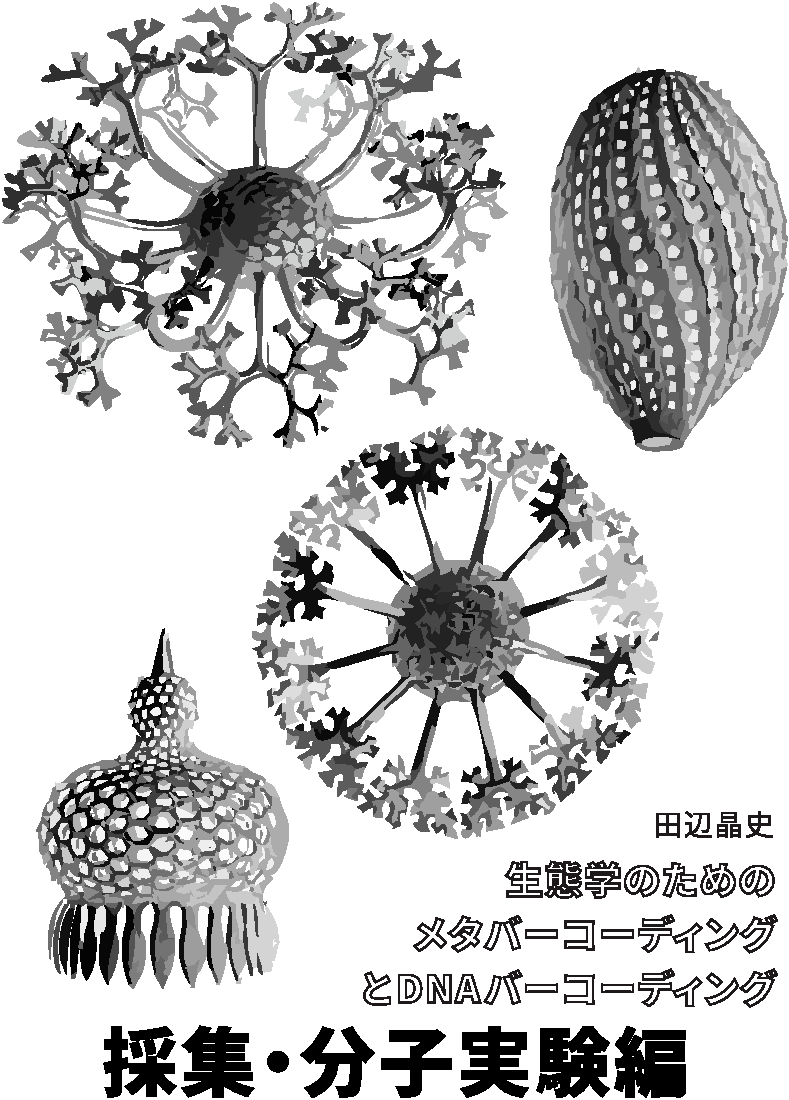
\includegraphics[pagebox=cropbox,clip]{metabarcodingtextbook1.ja.title.pdf}\end{center}%
  \cleardoublepage
  \begin{titlepage}%
    \let\footnotesize\small
    \let\footnoterule\relax
    \let\footnote\thanks
    \null\vfil
    \vskip 60\p@
    \begin{center}%
      {\LARGE \@title \par}%
      \vskip 3em%
      {\large
        \lineskip .75em
        \begin{tabular}[t]{c}%
          \@author
        \end{tabular}\par}%
      \vskip 1.5em
      {\large \@date \par}%
    \end{center}%
    \par
    \@thanks\vfil\null
  \end{titlepage}%
  \setcounter{footnote}{0}%
  \global\let\thanks\relax
  \global\let\maketitle\relax
  \global\let\@thanks\@empty
  \global\let\@author\@empty
  \global\let\@date\@empty
  \global\let\@title\@empty
  \global\let\title\relax
  \global\let\author\relax
  \global\let\date\relax
  \global\let\and\relax
}
\makeatother

\title{生態学のためのメタバーコーディングとDNAバーコーディング:採集・分子実験編}
\author{田辺晶史}
\date{\today}

%\renewcommand{\baselinestretch}{1.2}
\renewcommand{\prepartname}{第}
\renewcommand{\postpartname}{部}
\renewcommand{\prechaptername}{第}
\renewcommand{\postchaptername}{章}
\renewcommand{\presectionname}{}%  第
\renewcommand{\postsectionname}{}% 節
\renewcommand{\contentsname}{目次}
\renewcommand{\listfigurename}{図目次}
\renewcommand{\listtablename}{表目次}
\renewcommand{\refname}{引用文献}
\renewcommand{\bibname}{引用文献}
\renewcommand{\indexname}{索引}
\renewcommand{\figurename}{図}
\renewcommand{\tablename}{表}
\renewcommand{\appendixname}{付録}

\usepackage{float}
\usepackage{framed}
\definecolor{shadecolor}{gray}{0.9}
\newenvironment{content}{\begin{shaded}\vspace{-1em}\raggedright\ttfamily\footnotesize\setlength{\baselineskip}{1.4em}}{\end{shaded}\vspace{-1em}}
\newenvironment{pre}{\begin{leftbar}\raggedright\ttfamily\footnotesize\setlength{\baselineskip}{1.4em}}{\end{leftbar}\vspace{-1em}}
\newenvironment{cmd}{\begin{oframed}\raggedright\ttfamily\footnotesize\setlength{\baselineskip}{1.4em}}{\end{oframed}\vspace{-1em}}

\setlength{\textwidth}{\fullwidth}
\setlength{\evensidemargin}{\oddsidemargin}
\addtolength{\evensidemargin}{-2.5 true mm}
\addtolength{\oddsidemargin}{2.5 true mm}

\makeatletter
\renewcommand{\chapter}{%
  \if@openright\cleardoublepage\else\clearpage\fi
  \global\@topnum\z@
  \secdef\@chapter\@schapter}
\makeatother

\renewcommand{\textbf}[1]{{\bfseries\sffamily#1}}

\bibliographystyle{jecon}

\begin{document}
\thispagestyle{empty}
\maketitle
\cleardoublepage
\pagenumbering{roman}
\tableofcontents
\cleardoublepage
\setlength{\parindent}{0em}
\setlength{\parskip}{1em plus 0.2em}
\parindent=0em
\parskip=1em plus 0.2em
\pagenumbering{arabic}

\chapter*{はじめに}
\addcontentsline{toc}{chapter}{はじめに}

本書はクリエイティブ・コモンズの表示-継承 4.0 国際ライセンスの下で配布します。
このライセンスの下では、原著作者の明示を行う限り、利用者は自由に本書を複製・頒布・展示することができます。
また、原著作者の明示と本ライセンスまたは互換性のあるライセンスの適用を行う限り、本書を改変した二次著作物の作成・配布も自由に行うことができます。
詳しい使用許諾条件を見るには\\
\href{https://creativecommons.org/licenses/by-sa/4.0/}{https://creativecommons.org/licenses/by-sa/4.0/}\\
をチェックするか、クリエイティブ・コモンズに郵便にてお問い合わせ下さい。
住所は Creative Commons, PO Box 1866, Mountain View, CA 94042, USA です。

本書が皆さんの役に立つことができましたら幸いです。
この機会を与えて下さった京都大学生態学研究センターの東樹宏和博士、宇野裕美博士、神戸大学の末次健司博士、佐藤拓哉博士、水産研究・教育機構中央水産研究所の長井敏博士、龍谷大学の山中裕樹博士、東北大学の近藤倫生博士と、本書をお読みの皆さんに感謝します。

\chapter{環境DNA・メタゲノムDNAの採集方法}

ここでは、水からの環境DNA採集、および水、土壌、糞などからのメタゲノムDNAの採集方法について解説します。
DNA抽出用の個体や組織の採集方法はここでは取り扱いません。
なお、環境DNAとメタゲノムDNAは識別困難ですが、ここでは、環境DNAを「生物個体から排出されたDNA」、メタゲノムDNAを「生物個体から排出されていないDNA」ということにします。
したがって、水中の魚類や甲殻類、水生昆虫、水生植物のDNAは環境DNAであり、微生物のDNAはメタゲノムDNAであることが多いでしょう(ただし、区別できないだけで微生物の環境DNAも含まれているでしょう)。
また、未消化物に含まれる被食者や本人のDNAはどちらにするか難しいところですが、とりあえずメタゲノムDNAということにしておきます。

\section{サンプリングデザイン}

採集地点・時間をどのように配置するかは研究の内容に直結する重要な課題です。
ここで研究目的の達成の可否が決まると言っても過言ではありません。
そのためには、研究目的の明確化と予備調査が必須です。

例えば、ため池ごとの魚類相と環境条件(池の大きさ、深さ、水質、地質、高度、緯度経度など)との関連性を解明したいが、ため池の中での微細な違いには興味がないケースでは、ため池がよほど小さくない限り、ため池内の数地点から水を採集し、混合して濾過採集することになります。
ため池が非常に小さい場合や、ため池内の水が十分に混合されていたり、対象となるため池があまりに多い場合は、1地点だけでため池を代表させることもあるでしょう。
もちろん、余裕があるならため池内の数地点のサンプルを全て別々にして、その気になればため池内の微細な違いをも解析可能にしておくことも悪くありませんが、後述するサンプルレプリケートを複数用意することを考えると、大きな労力が必要となりますので、人手を十分考慮する必要があります。
また、その場合はため池内の数地点のサンプル間でDNA抽出効率・PCR増幅効率などに大きな違いが生じることがないようにしなくてはなりません(違う場合は環境条件の影響と言えなくなってしまう)。

別のケースとして、森林の土壌を分析して、微生物叢と植物相の関連性を解明したい場合を考えましょう。
この場合、1地点を広くかつ深く取り、その範囲の土壌を混合して採集するか、その範囲の土壌からいくつかのサブサンプルを採集して混合するのがよいでしょう。
土壌では、少し離れただけで全く異なる微生物叢を示すので、ある場の植物相と対応する微生物叢を完全な1点では代表することができません。
そのため、植物相と対応する範囲の数地点のサブサンプルをプールすることで代表させます。

以上のように、「DNAの拡散する範囲」と「そのサンプルで代表させたい範囲」を考慮して、前者の範囲の方が広くなるようにサンプリングデザインを行う必要があります。
後者の範囲の方が広くなってしまう場合、研究の目的とする議論が行えなくなることがあります。
ただ、後者の範囲の方が広くなる場合でも、サンプルが大量にあるのであれば、「本来の生物相」と「サンプルの生物相」との乖離に何らかの偏りがない限りは目的の議論ができる場合もあるでしょう。

また、濾過採集を行う場合、濾過水量も結果に大きな影響を及ぼすことが知られています。
ただ、無制限に濾過水量を増やすことは不可能なため、現実的に実施可能な範囲で最大の水量を濾過するようにしている例が多いようです。

\section{テクニカルレプリケートについて}

1サンプルを1レプリケートで採集した場合、DNA抽出効率やPCR増幅効率のばらつきの影響を受けます。
また、レアな種のゲノムDNAや低濃度の環境DNAはサンプルに入ったり入らなかったりすることもあり得ます。
そこで、可能であれば複数(3以上ならなお良い)のレプリケートを1サンプル中に用意することが望ましくなります。
このようにすることで、各サンプルごとに種の「発見率」を推定することができます。
例えば、1サンプルが10レプリケート含んでいるとき、x軸をレプリケート数、y軸を合計種数とする折れ線グラフを描くことを想像して下さい。
10レプリケートからx軸のレプリケート数だけ無作為抽出して合計種数を算出してy軸の合計種数を計算します。
このとき、折れ線が傾きゼロの直線なら1レプリケートでも発見率は100\%と考えられ、x=1では傾きゼロではなくとも、x=10では傾きゼロになっているなら10レプリケート合計すれば飽和している=発見率100\%ということになります。
しかし、x=10でも線が傾いているようであれば、発見率は100\%ではなく、いくらか取りこぼしがあることがわかります。
発見率が100\%であることが理想ですが、必ずしもそうである必要はありません。
重要なのは、発見率が推定できることです。

\section{ネガティブコントロールについて}

この先の分析では、サンプル間のコンタミネーションを完全に防ぐことは難しいため、それを検出し、コンタミネーションの程度を推定できるよう、ネガティブコントロールサンプルを適宜作成することが求められます。
よく勘違いしている人がいますが、ネガティブコントロールの目的は、「コンタミネーションの程度を推定する」ことであって、「コンタミネーションが一切ないことを確認できるようにすること」ではありません(やってみればわかりますが、実際にはほぼ不可能で現実的ではありません)。
野外調査の際は、対象とする環境DNAが含まれていないと考えられる水(アズワン 工業用精製水 A300 (2-961-01)を推奨。コックまで付属していながら安価で大容量)を用意しておき、サンプルの水と同じ手順で濾過することでネガティブコントロールとします。
なお、研究室で予めプラスチックバッグに詰めて持っていってしまうと、プラスチックバッグに水を詰めるまでに経由する機材(使い捨てビーカーや「空気」)へのコンタミネーションの程度がわからなくなってしまうので、ネガティブコントロールとしては適切ではありません。
ネガティブコントロールは「サンプルの水と同じ手順で濾過する」ことが必要であることに注意して下さい。

\section{水からの濾過採集方法}

\subsection{濾過フィルターの選定}

メタゲノム・環境DNA採集に適した濾過フィルターには、形状・材質・粒子保持能で分けると以下の種類があります。ディスクフィルターはひとまず47mmのものを挙げておきますが、より小さいものや大きいものもあります。

\begin{itemize}
\item カートリッジ型フィルター
\begin{itemize}
\item PVDF製濾過膜
\begin{itemize}
\item 0.45{\textmu}m Millipore Sterivex-HV SVHV010RS
\item 0.22{\textmu}m Millipore Sterivex-GV SVGV010RS
\end{itemize}
\item PES製濾過膜
\begin{itemize}
\item 0.22{\textmu}m Millipore Sterivex-GP SVGP01050
\end{itemize}
\end{itemize}
\item 47mmディスクフィルター
\begin{itemize}
\item グラスファイバー製濾紙
\begin{itemize}
\item 1.2{\textmu}m Whatman GF/C 1822-047
\item 0.7{\textmu}m Whatman GF/F 1825-047
\item 0.7{\textmu}m Millipore AP40 AP4004705
\end{itemize}
\item ポリカーボネート製濾過膜
\begin{itemize}
\item 12.0{\textmu}m Whatman Nuclepore 111116
\item 10.0{\textmu}m Whatman Nuclepore 111115
\item 10.0{\textmu}m Millipore Isopore TCTP04700
\item 8.0{\textmu}m Millipore Isopore TETP04700
\item 5.0{\textmu}m Millipore Isopore TMTP04700
\item 3.0{\textmu}m Whatman Nuclepore 111112
\item 3.0{\textmu}m Millipore Isopore TSTP04700
\item 2.0{\textmu}m Whatman Nuclepore 111111
\item 2.0{\textmu}m Millipore Isopore TTTP04700
\item 1.2{\textmu}m Millipore Isopore RTTP04700
\item 1.0{\textmu}m Whatman Nuclepore 111110
\item 0.8{\textmu}m Millipore Isopore ATTP04700
\item 0.6{\textmu}m Millipore Isopore DTTP04700
\item 0.4{\textmu}m Millipore Isopore HTTP04700
\item 0.22{\textmu}m Millipore Isopore GTTP04700
\end{itemize}
\item セルロース混合エステル製濾過膜
\begin{itemize}
\item 8.0{\textmu}m Millipore MF-Millipore SCWP04700
\item 5.0{\textmu}m Millipore MF-Millipore SMWP04700
\item 3.0{\textmu}m Millipore MF-Millipore SSWP04700
\item 1.2{\textmu}m Millipore MF-Millipore RAWP04700
\item 0.8{\textmu}m Millipore MF-Millipore AAWP04700
\item 0.65{\textmu}m Millipore MF-Millipore DAWP04700
\item 0.45{\textmu}m Millipore MF-Millipore HAWP04700
\item 0.3{\textmu}m Millipore MF-Millipore PHWP04700
\item 0.22{\textmu}m Millipore MF-Millipore GSWP04700
\end{itemize}
\item PVDF製濾過膜
\begin{itemize}
\item 0.45{\textmu}m Millipore Durapore HVLP04700
\item 0.22{\textmu}m Millipore Durapore GVWP04700
\end{itemize}
\item PES製濾過膜
\begin{itemize}
\item 0.45{\textmu}m Millipore Millipore Express PLUS HPWP04700
\item 0.22{\textmu}m Millipore Millipore Express PLUS GPWP04700
\end{itemize}
\end{itemize}
\end{itemize}

カートリッジ型の方が事前に塩素漂白しないといけないものが少なく準備が楽で、コンタミネーションはしにくいと考えられます。
ただし高価で濾過膜の選択肢が少ないというデメリットがあります。
ディスクフィルターは事前に塩素漂白しないといけないものが多いため準備の手間が多く、コンタミネーションしやすいですが、その代わり安価で濾過膜の選択肢が多くあります。
保存時の占有スペースはディスクフィルターの方が圧倒的に小さいので、冷凍庫により多く入れられます。

ポリカーボネート製濾過膜は孔径が極めて均一で粒子サイズごとの分画に適し、様々な孔径の品が揃えられています。
デメリットとしては、空隙率が低く濾過が遅い、目詰まりしやすい、そして高価という点があります。
セルロース混合エステルは孔径はポリカーボネートほど均一ではありませんが、孔径の選択肢は多く、空隙率が非常に高いため濾過が早い上、ポリカーボネートに比べれば安価です。
ポリエーテルスルホン(PES)とポリフッ化ビニリデン(PVDF)も空隙率が高く濾過はポリカーボネートよりずっと早くなります。
グラスファイバーもポリカーボネートに比べて空隙率が高く濾過はずっと早いですが、孔径の均一性は最も低く、その上DNA・RNAを吸着しやすい性質があります(DNA・RNAの抽出にも利用されるくらいです)。
しかし、グラスファイバーが最も安価です。

また、濾過フィルターの選択はDNAの抽出方法にも影響を及ぼします。
カートリッジ型の場合、バッファーを注入してインキュベートすることでバッファー中にDNAを溶解させ、逆さまにして遠心することで回収します\citep{Miya2016}。
微生物メタゲノムの場合、ジルコニアビーズなどをカートリッジ内に入れて破砕処理を加えることで抽出効率を改善することもできます\citep{Ushio2019}。
ディスクフィルターからの環境DNAの回収では、最初にフィルターを筒状に丸めてSalivetteや空カラム(吸着剤の入っていないスピンカラム)に入れ、そこにバッファーを加えてインキュベートすることでDNAを溶解します。
ディスクフィルターから微生物メタゲノムを回収する場合、バッファー中でフィルターを切り刻んでジルコニアビーズを加えて破砕処理を行います。
このため、グラスファイバー製などの剪刀で刻みにくいフィルターは使用できません。

\subsection{濾過方法の選定}

濾過の方法には、以下の4通りがあります。

\begin{enumerate}
\item シリンジを用いて手動で加圧する
\item 真空ポンプを手動で動かして吸引する
\item ペリスタルティックポンプなどを電気で動かして加圧する
\item 真空ポンプを電気で動かして吸引する
\end{enumerate}

どの方法を用いても構いませんが、電気が使えない場所では1を、電気が使える場所では4を使うのが主になると思います。
採水後にすぐには濾過できない場合、10\%塩化ベンザルコニウム溶液(オスバンSという名前で薬局で販売されている)を1L当たり1mL加える(終濃度0.01\%)ことで、細菌による環境DNAの分解を抑制できるという報告\citep{Yamanaka2017}があり、近年よく利用されているようです。

\subsection{濾過量の決定}

濾過量は基本的には多ければ多いほど良いのですが、時間的・労力的制約が存在するため、ある程度の量で妥協することになります。
Sterivexを使用する場合、海洋では1L、淡水では500mLとすることが多いようです。
ただし、プランクトンや鉱物粒子が多い場合は250mL程度が限界となるケースもあります。
逆に、河川最上流域や海洋の沖合では、数Lの濾過を行うことも可能です。
濾過量がばらついてしまう場合、複数のフィルターを用いて濾過量を均一化する場合もあれば、濾過量を記録しておいて解析時に対応するケースもあります。
複数のフィルターを用いる場合、DNA抽出後にDNA溶液をまとめてしまうケースが多いと思います。
どうするのが最適かはケースごとに異なると思いますが、最適条件を探索するのは容易ではありません。
現実的には、正しく記録をする限りにおいて、どの方法を用いても問題はない、とせざるを得ないでしょう。

\subsection{サンプル固定方法の選定}

濾過サンプルの固定方法は、主に以下の方法が考えられます。

\begin{enumerate}
\item 可能な限り水抜きしてDNA・RNA固定液(作成法は付録\ref{makingRNAlater}を参照)を加える
\item 可能な限り水抜きしてTEバッファーを加える
\item 可能な限り水抜きしてエタノールを加える
\item 可能な限り水抜きして冷凍する
\end{enumerate}

最近の論文を読む限りでは、1と4がよく使われているようです。4以外は冷蔵、あるいは常温保管することも可能です。

\subsection{濾過採集関連機材の塩素漂白の方法}

\subsubsection{必要な機材}
\begin{itemize}
\item 水道
\item 蛇口に適合するシリコンチューブ (厚さは任意): 1本
\item 漂白剤抜き器 (作成方法は付録\ref{makingdebleachcontainer}を参照): 1個
\item 漂白対象物が入る大きさの容器: 1個
\item 防水エプロン: 1着
\item ショーワグローブ No.140 腕カバー付厚手: 1双
\end{itemize}

\subsubsection{必要な消耗品}
\begin{itemize}
\item 花王 ハイターE (界面活性剤なしの塩素系漂白剤。次亜塩素酸ナトリウム6\%): 適量
\item SPW: 適量
\end{itemize}

\subsubsection{作業手順}
\begin{enumerate}
\item 漂白対象物が入る大きさの容器に漂白対象物を入れる
\item 次に注ぐ水道水の2~10\%量のハイターEを入れる
\item 漂白対象物が浸かるように水道水を注ぐ
\item 漂白対象物が水に浮く場合、同サイズの容器を重ねて重しを入れて押さえつける (これができるような形状の容器を使用する)
\item 時々ゆすりながら10分以上、できれば1時間以上浸ける (ただし浸け過ぎに注意)
\item 漂白液を捨てて漂白対象物を漂白剤抜き器に移す
\item 漂白剤抜き器のホースニップルと水道の蛇口をシリコンチューブで接続する
\item 水道水を上限まで注いで捨てる
\item 漂白対象物が
\begin{enumerate}
\item 水に浮く場合、水道水を勢いよく流しっぱなしにして30分以上放置して水を捨てる (水の勢いで漂白対象物がぐるぐる動くようにする)
\item 水に沈む場合、水道水を上限まで注いで捨てることを更に2回繰り返す
\end{enumerate}
\item 漂白対象物が入る大きさの容器に漂白対象物を移す
\item SPWを漂白対象物が浸かるように注いですすいで捨てる
\item 乾燥が必要な場合はアルミホイルに包んで常温~60℃で乾燥する (60℃にする前に一度200℃以上で庫内を滅菌してから60℃に下げること)
\end{enumerate}

なお、漂白剤抜き器を漂白対象物が入る大きさの容器として使用しても問題ありません。
また、全ての作業を同じ容器(漂白剤抜き器を含む)で行っても構いません。
フィルターホルダーはパッキンやアダプターを外して分解し、個別に漂白を行い、漂白後に組み立てます。

\subsection{使い捨てビーカー・折りたたみバケツ・ポリタンクを使用した採水の方法}

\subsubsection{必要な機材}
\begin{itemize}
\item 漂白済みポリタンク: 1個 / 1サンプル
\item 漂白済み折りたたみバケツ: 1個 / 1サンプル
\item 漂白済みロープ(長さは任意): 1本 / 1サンプル
\end{itemize}

\subsubsection{必要な消耗品}
\begin{itemize}
\item 以下のいずれかの使い捨てビーカー: 1個 / 1サンプル
\begin{itemize}
\item 大塚刷毛製造 補修用カップ 容器のみ 400mL 3221110400
\item 大塚刷毛製造 補修用カップ 容器のみ 600mL 3221110600
\item 大塚刷毛製造 補修用カップ 容器のみ 800mL 3221110800
\item ビッグ 調色ミキシングカップ 1000mL MK11L
\end{itemize}
\end{itemize}

\subsubsection{作業手順}
\begin{enumerate}
\item 水深、水面までの距離、濾過作業できる場所までの距離、濾過作業できるようになるまでの時間に応じて、以下の方法から選択する
\begin{enumerate}
\item 水面に手が届く場合、使い捨てビーカーで直接採水する
\item 橋の上など、足場が高い場合、ロープで上から下ろしたバケツで水を汲む
\item 濾過作業できる場所が遠い、またはすぐに濾過できない場合、ポリタンクに水を汲む。その際、水面までの距離や水深によっては使い捨てビーカーやバケツを使用してポリタンクに水を入れる
\end{enumerate}
\end{enumerate}

いずれの場合も、共洗いは最低2回以上行います。
また、漂白したロープには漂白剤が僅かながら残留していることが多いので(繊維が入り組んでいるため完全に抜くのは難しい)、共洗いのついでに一度現場の水に漬け込みます。
水を汲む際にも、ロープからの水ができるだけバケツ内に入らないように注意します。
筆者はモノタロウ 折りたたみ式バケツ (09514944)を使用していますが、大変安価な上、折りたたんだ状態で漂白剤抜き器として使用しているアスベル ユニックス キッチンボックス S-70にぴったり4個入り、漂白が大変楽に行えるのでおすすめです(折りたたんだ状態でもしっかり漂白できる構造です)。

\subsection{吸引濾過装置を用いた水からの微生物メタゲノムDNA・環境DNAの濾過採集方法}

\subsubsection{必要な機材}
\begin{itemize}
\item DC12Vのシガーソケット搭載車 または ACアダプター: 1個
\item 車載用吸引ポンプユニット (作成方法は付録\ref{makingpumpunit}を参照): 1個
\item 吸引濾過装置 (作成方法は付録\ref{makingfilteringunit}を参照): 1個
\item toolsisland 手動式オイルチェンジャー または メルテック オイルチェンジャー OC-060: 1個
\item アズワン 穴付きシリコン栓 8号 (1-7650-01) の両方の穴に 光 ステンレス丸パイプ 外径6mm を適当な長さに切断して挿したもの (長さを不揃いにすること): 1個
\item アズワン シリコンチューブ 内径5mm 外径11mm 長さ1m (6-586-19-01): 1本
\item アズワン シリコンチューブ 内径5mm 外径11mm 長さ1m (6-586-19-01) を切断して途中に Whatman VACU-GUARD (6722-5000) を挟んだもの: 1本
\item モンキーレンチ: 1本 (ディスクフィルター使用時のみ)
\item サンダイヤ デッキ型ピンセット 125mm (アズワン品番 6-531-12): 1本 (ディスクフィルター使用時のみ)
\item ハサミ: 1本
\item ライター: 1本
\item ゼブラ マッキープロ細字 特殊用途DX: 1本 (色の薄いハズレ個体がよくあるので予め確認しておく)
\item 三菱アルミニウム 三菱ホイル タフ 30cm x 50m: 1本
\item ロゴス ハイパー氷点下クーラーM No.81670070: 1個
\item ロゴス 倍速凍結・氷点下パックXL No.81660640: 2個以上 (必ず氷点下を維持できる保冷剤を使用すること)
\end{itemize}

\subsubsection{必要な消耗品}
\begin{itemize}
\item 以下のいずれかの濾過フィルターユニット: 1個 / 1サンプル
\begin{itemize}
\item アズワン FH-PP47 (3-6736-01) または ADVANTEC PP-47 に47mmディスクフィルターを詰めたもの (漂白で再利用可)
\item Millipore Sterivex-HV 0.45{\textmu}m PVDF SVHV010RS
\item Millipore Sterivex-GV 0.22{\textmu}m PVDF SVGV010RS
\item Millipore Sterivex-GP 0.22{\textmu}m PES SVGP01050
\end{itemize}
\item Sterivex使用時に出口側に付ける10{\textmu}Lチップ (フィルターなし)
\item フィルターユニットに適合するアダプター (作成方法は付録\ref{makingfilteradapter}を参照): 1個 / 1サンプル (漂白で再利用可)
\item 以下のいずれかのプラスチックバッグ: 1個 / 1サンプル
\begin{itemize}
\item カウパック 夢パック 100mL DP16-TN0100
\item カウパック 夢パック 200mL DP16-TN0200
\item カウパック 夢パック 300mL DP16-TN0300
\item カウパック 夢パック 500mL DP16-TN0500
\item カウパック 夢パック 1000mL DP16-TN1000
\end{itemize}
\item 以下のいずれかの使い捨てビーカー: 1個 / 1サンプル
\begin{itemize}
\item 大塚刷毛製造 補修用カップ 容器のみ 400mL 3221110400
\item 大塚刷毛製造 補修用カップ 容器のみ 600mL 3221110600
\item 大塚刷毛製造 補修用カップ 容器のみ 800mL 3221110800
\item ビッグ 調色ミキシングカップ 1000mL MK11L
\end{itemize}
\item セイニチ ユニパック C-4: 1枚 / 1サンプル
\item 使い捨てポリ手袋: 2双 / 1サンプル
\end{itemize}

\subsubsection{作業手順}
\begin{enumerate}
\item 車載用吸引ポンプユニットのバルブは開放しておく
\item 吸引濾過装置のバルブは全て閉じておく
\item シガーソケットに車載用吸引ポンプユニットの電源を接続する
\item 車載用吸引ポンプユニットのホースニップルにVACU-GUARDを取り付けたシリコンチューブ経由で穴付きシリコン栓の短い方のステンレスパイプを接続する
\item 穴付きシリコン栓を手動式オイルチェンジャーのタンクに挿す
\item 穴付きシリコン栓の長い方のステンレスパイプにもう一つのシリコンチューブ経由で吸引濾過装置を接続する
\item ポリ手袋を着ける
\item 使い捨てビーカーで必要量の水試料を量り取り、プラスチックバッグに入れる
\item 濾過フィルターユニットにアダプターを取り付ける (ディスクフィルター使用の場合はモンキーレンチでしっかり締め付ける)
\item Sterivexの場合は出口側に10{\textmu}Lチップを取り付け、Sterivexが直接濾過器に触れないようにする
\item アダプターの反対側に水試料の入ったプラスチックバッグを取り付ける (アダプターの接着面に力がかからないように注意すること)
\item プラスチックバッグ+濾過フィルターユニットを濾過フィルターユニットが下になるように吸引濾過装置に取り付け、リピートバンドを締める
\item 吸引濾過装置のバルブ(プラスチックバッグからタンクの経路上のもの)を開ける
\item 車載用吸引ポンプユニットの電源を入れ、水試料を吸引する
\item 水試料吸引開始後、プラスチックバッグ上端にハサミで切り込みを入れる (ハサミが水試料に接さないように注意。必要に応じてハサミをライターで火炎滅菌する)
\item 水試料の吸引が終わったら、吸引濾過装置の濾過フィルターユニット直下のバルブを閉じる
\item リピートバンドを緩めてプラスチックバッグ+濾過フィルターユニットを吸引濾過装置から外す
\item 濾過フィルターユニットからプラスチックバッグを取り外して捨てる (アダプターは残す)
\item 濾過フィルターユニットを再度吸引濾過装置に取り付け、濾過フィルターユニット直下のバルブを開けて濾過フィルターユニット内の残留水を吸引する (濾過フィルターユニットを独楽のように回して吸引する)
\item アルミホイルを適当な長さで切って折り目を付けておく
\item 吸引濾過装置の濾過フィルターユニット直下のバルブを閉じて車載用吸引ポンプユニットの電源を切る
\item 濾過フィルターユニットを吸引濾過装置から外す
\item ポリ手袋を交換する
\item 濾過フィルターユニットが
\begin{enumerate}
\item フィルターホルダー+ディスクフィルターの場合、アダプターはそのままにして分解し、フィルターを分解してライターで火炎滅菌したピンセットで濾液入力面を内側にして二つ折りにし、アルミホイルで包んでマッキープロでサンプル情報を記述しユニパックに入れ、クーラーバッグに保冷剤で挟まれるように入れる
\item Sterivexの場合、アダプターを外してマッキープロでサンプル情報を記述し、アルミホイルで包んでから(省略可)ユニパックに入れ、クーラーバッグに保冷剤で挟まれるように入れる (ユニパックにもサンプル情報を記述しておく)
\end{enumerate}
\item ポリ手袋を外して捨てる
\item 吸引濾過装置の下部バルブを両方共開放する (吸引濾過装置内の残留水がタンクに吸い込まれる)
\item 手動式オイルチェンジャーのタンクからシリコン栓を外し、中の廃液を捨てる
\end{enumerate}

\subsubsection{記述しておくべきサンプル情報}
\begin{itemize}
\item 採集地点
\item 採水日時
\item 濾過日時
\item 濾過量
\item フィルター材質
\item フィルター粒子保持能
\end{itemize}

なお、アズワンFH-PP47およびADVANTEC PP-47のパッキンが劣化した場合、シリコンゴムかフッ素ゴム製のAS568-030型およびAS568-033型の品に交換することができます。

ここではSterivexをすぐに冷凍する方法を示しましたが、中にDNA・RNA固定液(作成法は付録\ref{makingRNAlater}を参照)を注入して両端にキャップ(テルモ テルフュージョン三方活栓キャップ密栓用 XX-WS01K* および コクゴ 点眼キャップ赤3φ 101-5210102)を付けて冷凍・冷蔵・常温保管する方法もあります(DNA・RNA固定液を注入しない場合もDNA抽出時にはキャップを使用することになるので、採集時に付けておくのも良いでしょう)。
海外などで冷凍手段が確保できない場合にはこの方法を用いることになります。

\subsection{シリンジを用いた水からのメタゲノムDNA・環境DNAの濾過採集方法}

\subsubsection{必要な機材}
\begin{itemize}
\item コーキングガン タジマ コンボイVS CNV-VS: 1個 (先端の円筒部内側に、ワッシャーがくっつくようコクヨ マク-S340をカットして貼っておく。また、ベスト 黒ゴム平置き 40ミリをハサミで数mm程度小さくし、押し子に接着しておく)
\item ゼブラ マッキープロ細字 特殊用途DX: 1本 (色の薄いハズレ個体がよくあるので予め確認しておく)
\item 三菱アルミニウム 三菱ホイル タフ 30cm x 50m: 1本
\item ロゴス ハイパー氷点下クーラーM No.81670070: 1個
\item ロゴス 倍速凍結・氷点下パックXL No.81660640: 2個以上 (必ず氷点下を維持できる保冷剤を使用すること)
\item 大阪魂 丸ワッシャー 特寸 鉄/ユニクロ M21 x 外径50mm x 厚さ3.2mm 4個入 (42175375) または 同 70個入 (41954954): 1枚 (予めアルミホイルで包んで乾熱滅菌しておく)
\item シンワ測定 数取器 台付 75078 または 新潟精機 数取器 台付型 C-4B: 1個
\end{itemize}

\subsubsection{必要な消耗品}
\begin{itemize}
\item テルモ テルモシリンジ ロック付 50mL SS-50LZ: 1本 / 1サンプル
\item 以下のいずれかの濾過フィルターユニット: 1個 / 1サンプル
\begin{itemize}
\item Millipore Sterivex-HV 0.45{\textmu}m PVDF SVHV010RS
\item Millipore Sterivex-GV 0.22{\textmu}m PVDF SVGV010RS
\item Millipore Sterivex-GP 0.22{\textmu}m PES SVGP01050
\end{itemize}
\item 以下のいずれかの使い捨てビーカー: 1個 / 1サンプル
\begin{itemize}
\item 大塚刷毛製造 補修用カップ 容器のみ 400mL 3221110400
\item 大塚刷毛製造 補修用カップ 容器のみ 600mL 3221110600
\item 大塚刷毛製造 補修用カップ 容器のみ 800mL 3221110800
\item ビッグ 調色ミキシングカップ 1000mL MK11L
\end{itemize}
\item セイニチ ユニパック C-4: 1枚 / 1サンプル
\item 使い捨てポリ手袋: 1双 / 1サンプル
\end{itemize}

\subsubsection{作業手順}
\begin{enumerate}
\item ポリ手袋を着ける
\item ワッシャーの面が取れている方がSterivexに接するようコーキングガン先端にセットする
\item セットしたワッシャーが何かに触れないようにコーキングガンをどこかに吊り下げる
\item 手を使わずにボタンを押せるように数取器を設置する
\item 使い捨てビーカーで必要量の水試料を量り取る
\item シリンジにビーカーから水試料50mLを吸い取る (水に浸かるシリンジ先端3cm程度は触れないようにする)
\item シリンジのルアーロック部にSterivexを取り付ける
\item コーキングガン先端のワッシャーの穴からSterivexが突き出すようにセットする
\item Sterivexが下になるように垂直に立ててコーキングガンの引き金を引いて加圧濾過する (加圧しすぎると壊れるので、水が出るのを待つこと)
\item 50mLの濾過が終わったら、数取器のボタンを手を使わずに肘などで押してカウントアップする
\item シリンジ+Sterivexをコーキングガンから抜いてSterivexとシリンジを分離する
\item 必要量に達するまで6~11を繰り返す (濾過に必要な圧力が大きくなってきたら無理せず複数本に分ける)
\item シリンジに空気をめいっぱい吸引する
\item シリンジのルアーロック部にSterivexを取り付けてワッシャーに通す
\item Sterivexが先端から突き出すようにコーキングガンにセットする
\item Sterivexが下になるように垂直に立ててコーキングガンの引き金を引き、できるだけSterivex内の水を抜く
\item シリンジ+Sterivexをコーキングガンから抜いてSterivexとシリンジを分離する
\item 13~17を3回程度繰り返して、できるだけSterivex内の水を抜く
\item Sterivexをアルミホイルで包んでから、マッキープロでサンプル情報を記述したユニパックに入れ、クーラーバッグに保冷剤で挟まれるように入れる
\item ポリ手袋を外して捨てる
\end{enumerate}

\subsubsection{記述しておくべきサンプル情報}
\begin{itemize}
\item 採集地点
\item 採水日時
\item 濾過日時
\item 濾過量
\item フィルター材質
\item フィルター粒子保持能
\end{itemize}

水中の粒子が少ない場合、コーキングガンを用いずに手で加圧して濾過した方が早いため、それが難しくなるくらい目詰まりするまでは手でやった方がいいでしょう。
コンボイVSでは、ワッシャーを用いずにシリンジ+Sterivexをコーキングガンにセットすることも可能ですが、シリンジ+Sterivexの水に接触した部分がコーキングガンに触れないよう注意してセットする必要があります。

シリンジには100mLタイプ(JMS JS-S00L)もあります。
高価ですが、濾過作業の反復数を半減させることができます。
これを用いる場合、金属製のワッシャーの代わりに、呼び径40の塩ビVP管(内径40.8mm・外径48mm)を15mmの長さに切断したものを使用します。
塩ビ管は予め塩素漂白してアルミホイルで個包装しておきます。
50mLシリンジとワッシャーの組み合わせでは、ワッシャーからはSterivexだけが突き出る形になりますが、100mLシリンジと塩ビ管の組み合わせでは、Sterivexとシリンジの先端半分以上が塩ビ管から突き出るようにして、塩ビ管でフランジを支えます。
なお、ここで挙げたタジマのコンボイVS以外のコーキングガンでは、100mLシリンジの太さには対応できない(39mmのシリンジ外筒を通せない)ものが多いのでご注意願います。

ここではSterivexをすぐに冷凍する方法を示しましたが、中にDNA・RNA固定液(作成法は付録\ref{makingRNAlater}を参照)を注入して両端にキャップ(テルモ テルフュージョン三方活栓キャップ密栓用 XX-WS01K* および コクゴ 点眼キャップ赤3φ 101-5210102)を付けて冷凍・冷蔵・常温保管する方法もあります(DNA・RNA固定液を注入しない場合もDNA抽出時にはキャップを使用することになるので、採集時に付けておくのも良いでしょう)。
海外などで冷凍手段が確保できない場合にはこの方法を用いることになります。

\chapter{DNA抽出・ライブラリ調製・シーケンシング}

\section{機材・試薬の滅菌とDNA分解によるコンタミネーションの抑制}

ピペットで使用するチップは全てフィルターチップにします。
ただし、DNAを含む溶液を吸わない場合にはフィルターのないチップを使っても構いません。
例えば、10mLチップでDNAを含む溶液を吸うことは考えにくいので、10mLチップはフィルターなしで問題ないと思います。

使用する機材や試薬は、以下のようにいくつかの方法を用いて滅菌およびDNA分解を行うことでコンタミネーションを抑制します。

\begin{description}
\item[金属製機材] オーブンを用いて乾熱滅菌する。250℃で30分。または紫外線滅菌30分。
\item[ガラス製機材] オーブンを用いて乾熱滅菌する。230℃で1時間。または紫外線滅菌30分。
\item[フッ素樹脂製機材] オーブンを用いて乾熱滅菌する。250℃で30分。または紫外線滅菌30分。
\item[フェノール樹脂製機材] オーブンを用いて乾熱滅菌する。200℃で4時間。
\item[PBT樹脂製機材] オーブンを用いて乾熱滅菌する。180℃で8時間。または紫外線滅菌30分。
\item[その他のプラスチック製機材] タライで塩素漂白する。20倍希釈漂白液で10分。または紫外線滅菌30分。
\item[乾熱滅菌、塩素漂白できない機材] DNA-OFFまたはDNA AWAYを染み込ませたペーパータオルで拭き取る。
\item[試薬] ガラス瓶に入れてオートクレーブ。
\item[クリーンベンチ] 紫外線滅菌30分。
\item[実験室] DNA-OFF、DNA AWAY、50ppm以上の次亜塩素酸水(次亜塩素酸ナトリウム溶液ではない)を染み込ませたペーパータオルで拭き取る。
\end{description}

ただし、当該処理を行うと著しく劣化したり分解する場合は行わないように注意が必要です(例えば、分解してしまうためPEG8000を含む溶液をオートクレーブしてはいけません)。
作業後の実験台やピペットはDNA-OFFかDNA AWAYを染み込ませたペーパータオルで拭き取ります。
作業後のプラスチック製チューブラックは塩素漂白します。
恒温槽のブロックや金属製のローターは水道水で洗浄してからSPWですすいで乾かし、紫外線を30分照射します。
インキュベータは250℃まで上げられるものであれば、250℃で30分ほど内部を乾熱滅菌します(それが可能なインキュベータを購入するようにします。「恒温乾燥器」とか「定温乾燥器」という名称で販売されています)。
次亜塩素酸水を使用する場合、分解しやすいので、200ppm以上の高濃度の品を半年以内に使い切るようにします(使用時に希釈します)。
漂白剤(次亜塩素酸ナトリウム溶液)、次亜塩素酸水、DNA-OFF、DNA AWAYが残留しないように注意して下さい。
漂白剤を抜くには、水道水で3回以上すすいでから、さらにSPWですすいで乾かします。
漂白剤以外は長期残留しませんが、DNA溶液に直接接するもの、それらに接するものの場合はSPWを染み込ませたペーパータオルで仕上げ拭きをした方が良いでしょう(実験台やピペットは該当しませんが、ピアシングするプレートシールは該当します)。

遠心機は、トミー精工のMDXシリーズを用いると、プラスチック製のローターが使用できるため、塩素漂白が可能です。
トミー精工MDXシリーズ用ローターTAR015-SC18と専用トレーTRA-01を使用すると、スピンカラムの頻繁な差し替えを減らし、廃液を1本ずつ捨てる作業をなくすことができます。
Salivette・Sterivexの遠心には、トミー精工LCX-200にTS-33CスイングローターとB433バケット、3315-TC04Pラックの組み合わせ(最大16本同時遠心可能)や、久保田商事S500T・S500FRにST-2504MSスイングローターと055-1160または055-1140ラックの組み合わせ(最大16または28本同時遠心可能)、Eppendorf Centrifuge 5804・5804R・5810・5810RにA-4-44スイングローター(Order no. 5804 709.004)と15mL遠沈管用アダプター(Order no. 5804 755.006)または17.5mm径チューブ用アダプター(Order no. 5804 754.000)の組み合わせ(最大16または24本同時遠心可能)が便利です。
これらの製品はラックがプラスチック製のため、塩素漂白が可能です(ただし、メーカーは推奨していない場合があります)。
スイングローターを使用するのは、Sterivexの中からの排液量・残液量を均一にし、再現性を高めるためです。
アングルローターでSterivexを遠心すると、排液が不完全・不均一になるため、おすすめできません。
なお、Eppendorf Centrifuge 5804・5804R・5810・5810Rは1.5・2mLチューブを20000×gで遠心できるアングルロータもあるので、1台でSalivette・Sterivex、1.5・2mLチューブやスピンカラムの遠心全てに対応できます。

DNA抽出・PCR前の準備を行う部屋と、PCRおよびPCR後の操作を行う部屋は分離し、相互に行き来をしない、あるいは行き来をする場合も各部屋専用の白衣、マスク、キャップを使用するなど、PCRによる増幅後のDNAのコンタミネーションに細心の注意を払う必要があります。
DNA抽出では汚れたものも扱うため、DNA抽出とPCR前の準備もできれば別の部屋に分けた方が良いでしょう。
クリーンベンチを活用すれば部屋の数は減らせますが、少なくともPCR前とPCR以降で2部屋は必要です。
筆者の場合、ディスクフィルターからのDNA抽出のためにフィルターを丸めてスピンカラムに入れたりSterivexにバッファーを入れる作業、PCRの前準備をしてから鋳型としてPCR産物を加える作業、の2つだけはクリーンベンチ内で行っています(軽いものが吹き飛んだりDNAが飛び散ったりしてしまうので、作業中にファンは使用しない。なお、この2つのクリーンベンチは、異なる部屋に設置された異なるクリーンベンチです)。

\section{ピペット操作と電動ピペット}

あとでかく。
リバースピペッティングを覚えること。

\section{テクニカルレプリケートとネガティブコントロール}

あとでかく。

\section{DNA抽出}

ここでは、自作バッファーと単体販売されているスピンカラムを組み合わせたDNA抽出方法を説明します。
既製のDNA抽出キットを用いる場合、QIAGENのDNeasy Blood \& Tissue Kit、またはSIGMA GenElute Mammalian Genomic DNA Miniprep Kit、またはNew England BioLabs Monarch Genomic DNA Purification Kitに置き換えることができます。
バッファー類の対応関係は下記の通りです。

\begin{itemize}
\item Insect Lysis Buffer
\begin{itemize}
\item QIAGEN Buffer ATL
\item SIGMA Lysis Solution T
\item New England BioLabs Monarch gDNA Cell Lysis Buffer
\end{itemize}
\item Binding Buffer
\begin{itemize}
\item QIAGEN Buffer AL
\item SIGMA Lysis Solution C
\item New England BioLabs Monarch gDNA Binding Buffer (アルコール類含有のため、別途エタノールは不要)
\end{itemize}
\item Wash Buffer 1
\begin{itemize}
\item QIAGEN Buffer AW1
\item SIGMA Wash Solution
\item New England BioLabs Monarch gDNA Wash Buffer
\end{itemize}
\item Wash Buffer 2
\begin{itemize}
\item QIAGEN Buffer AW2
\item SIGMA Wash Solution
\item New England BioLabs Monarch gDNA Wash Buffer
\end{itemize}
\item IDTE (溶出用)
\begin{itemize}
\item QIAGEN Buffer AE
\item SIGMA Elution Solution
\item New England BioLabs Monarch gDNA Elution Buffer
\end{itemize}
\end{itemize}

なお、SIGMA GenElute Mammalian Genomic DNA Miniprep Kitでは、カラム使用前にColumn Preparation Solutionを通す必要がありますので、忘れないようにご注意願います。

\subsection{固形サンプル(濾過フィルター以外)からのDNA抽出プロトコル}

必要な試薬の作成方法は付録\ref{makingDNAextractionbuffers}を参照して下さい。

\subsubsection{必要な機材}
\begin{itemize}
\item 恒温槽またはインキュベータ: 1台
\item 1.5・2mLチューブ20000×g対応遠心機: 1台
\item HOZAN ピンセット P-888: 1本
\item ライター: 1本
\item 100{\textmu}Lピペット: 1本
\item 200{\textmu}Lピペット: 1本
\item 1000{\textmu}Lピペット: 1本
\item 10mL電動ピペット エー・アンド・デイ MPA-10000: 1本 (吸引吐出速度は最低に設定)
\end{itemize}

\subsubsection{必要な試薬・消耗品}
\begin{itemize}
\item 2mLチューブ: 1本 / 8サンプル
\item 2mLチューブ: 1本 / 16サンプル
\item 1.5mLチューブ: 2本 / 1サンプル
\item 1.5mL DNA低吸着チューブ: 1本 / 1サンプル
\item EconoSpin IIa フタありOリングあり+2mL丸底チューブ EP-11201: 1セット / 1サンプル
\item 20mg/mL Proteinase-K: 10{\textmu}L / 1サンプル
\item Insect Lysis Buffer: 200{\textmu}L / 1サンプル (析出に注意)
\item Binding Buffer: 200{\textmu}L / 1サンプル (析出に注意)
\item Wash Buffer 1: 500{\textmu}L / 1サンプル
\item Wash Buffer 2: 500{\textmu}L / 1サンプル
\item 99.5\%エタノール: 200{\textmu}L / 1サンプル
\item IDTE: 120{\textmu}L / 1サンプル
\item サンプル組織片
\end{itemize}

\subsubsection{作業手順}
\begin{enumerate}
\item 恒温槽またはインキュベータを56℃に設定
\item Insect Lysis Buffer、Binding Bufferを加温して析出している結晶を溶かして転倒混和
\item Wash Buffer 1・2を冷凍庫から出して常温に戻しておく
\item 2mLチューブにInsect Lysis Buffer 200{\textmu}Lと20mg/mL Proteinase-K 10{\textmu}Lをサンプル数倍取って転倒混和してスピンダウン (最大8サンプル分/チューブ)
\item サンプル組織片を用意する
\item 1.5mLチューブに仮ラベルを振って、4を200{\textmu}Lずつ分注する
\item ピンセット先端を火炎滅菌する
\item 1個だけ6の1.5mLチューブの蓋を開ける
\item サンプルを6の1.5mLチューブに入れる
\item 7~9をサンプル数分繰り返す
\item 56℃で1時間以上インキュベートする
\item 新しい1.5mLチューブに仮ラベルを振って、Binding Buffer 200{\textmu}Lと99.5\%エタノール 200{\textmu}Lを入れておく
\item 新しいカラムにも仮ラベルを振っておく
\item 新しい1.5mL DNA低吸着チューブには正式なラベルを振っておく
\item 2mLチューブにIDTE 120{\textmu}Lをサンプル数倍+50{\textmu}L分注し、56℃に加温しておく (最大16サンプル分/チューブ)
\item インキュベートが1時間経ったら、11のチューブを20℃6000×gで1分遠心して上清を12のチューブに移してピペッティングして、混合液 600{\textmu}Lを新しいカラムに加える
\item カラムを20℃6000×gで1分遠心して\textbf{濾液を捨てる}
\item カラムにWash Buffer 1を10mL電動ピペットで500{\textmu}L加えて20℃6000×gで1分遠心し、\textbf{濾液を捨てる}
\item カラムにWash Buffer 2を10mL電動ピペットで500{\textmu}L加えて20℃20000×gで3分遠心する
\item エタノールを除去するため、20℃20000×gで更に1分遠心する (この濾液は捨てるが、後でよい)
\item 正式なラベルを振った1.5mL DNA低吸着チューブにカラムを移す (カラムに濾液が付着しないよう注意すること)
\item 15で加温しておいたIDTE 120{\textmu}Lをカラムの中心に加え、56℃で1分以上インキュベート (1サンプルごとにチップ交換)
\item 20℃6000×gで1分遠心し、\textbf{濾液を回収する}
\item -20℃で保管
\end{enumerate}

溶出処理の際の温度を管理することで、DNA回収率と再現性の向上を狙っています。

17以降の濾液の廃棄は、丸底チューブから適当な広口瓶に排液した後、アルミホイルの上にペーパータオルを引いて丸底チューブの口をペーパータオルに押し当てて水分を吸い取らせるようにします。
ペーパータオルはサンプル毎に替える必要はありませんが、コンタミネーションを防ぐためペーパータオルの使用位置は毎回ずらします。
アルミホイルの上にペーパータオルを引くのは実験台の汚れを防ぐためです。

10mL電動ピペットでWash Bufferを加える際、カラムからチップに跳ね返るとコンタミネーションの原因になってしまいます。
そのため、カラムを立てたラックの下に適当なものを挟んでラックとカラムを傾けて、Wash Bufferをカラム内壁に斜めに当たるようにします(吐出は鉛直に行います)。
電動ピペットの吐出速度も最低にセットします。
こうすることで、電動ピペットを用いて迅速にWash Bufferを加えることができます。

微生物メタゲノムDNAを抽出する場合、Proteinase-K処理のインキュベートを一晩に延ばし、インキュベート後に凍結融解を1~3回繰り返します。
凍結は液体窒素は用いず、{-20}~{-80}℃の冷凍庫に30分~1時間程度入れて行います(液体窒素による急速凍結では細胞が壊れにくい)。
必要に応じてビーズによる破砕処理を加えることで、収量が改善することがあります。
土壌サンプルなどでは、DNA抽出にスキムミルクやその有効成分であるカゼインを加えることで収量を改善できることが知られています\citep{Takada-Hoshino2004,Wang2012}。

\subsection{47mmディスクフィルター(グラスファイバー)からのDNA抽出プロトコル}

必要な試薬の作成方法は付録\ref{makingDNAextractionbuffers}を参照して下さい。

\subsubsection{必要な機材}
\begin{itemize}
\item 恒温槽またはインキュベータ: 1台
\item 1.5・2mLチューブ20000×g対応遠心機: 1台
\item HOZAN 逆作用ピンセット P-651: 1本
\item HOZAN ピンセット P-888: 1本
\item ライター: 1本
\item 100{\textmu}Lピペット: 1本
\item 200{\textmu}Lピペット: 1本
\item 1000{\textmu}Lピペット: 1本
\item 10mL電動ピペット エー・アンド・デイ MPA-10000: 1本 (吸引吐出速度は最低に設定)
\end{itemize}

\subsubsection{必要な試薬・消耗品}
\begin{itemize}
\item 2mLチューブ: 2本 / 8サンプル
\item 2mLチューブ: 1本 / 16サンプル
\item 1.5mLチューブ: 1本 / 1サンプル
\item 1.5mL DNA低吸着チューブ: 1本 / 1サンプル
\item EconoSpin 空カラム フタあり+2mL丸底チューブ EP-31201: 1セット / 1サンプル
\item EconoSpin IIa フタありOリングあり+2mL丸底チューブ EP-11201: 1セット / 1サンプル
\item 20mg/mL Proteinase-K: 10{\textmu}L / 1サンプル
\item Insect Lysis Buffer: 200{\textmu}L / 1サンプル (析出に注意)
\item Binding Buffer: 400{\textmu}L / 1サンプル (析出に注意)
\item Wash Buffer 1: 500{\textmu}L / 1サンプル
\item Wash Buffer 2: 500{\textmu}L / 1サンプル
\item 99.5\%エタノール: 400{\textmu}L / 1サンプル
\item IDTE: 200{\textmu}L / 1サンプル
\item IDTE: 120{\textmu}L / 1サンプル
\item 47mmディスクフィルターサンプル
\end{itemize}

\subsubsection{作業手順}
\begin{enumerate}
\item 恒温槽またはインキュベータを56℃に設定
\item Insect Lysis Buffer、Binding Bufferを加温して析出している結晶を溶かして転倒混和
\item Wash Buffer 1・2を冷凍庫から出して常温に戻しておく
\item 2mLチューブにInsect Lysis Buffer 200{\textmu}Lと20mg/mL Proteinase-K 10{\textmu}Lをサンプル数倍取って転倒混和してスピンダウン (最大8サンプル分/チューブ)
\item 2mLチューブにIDTE 200{\textmu}Lをサンプル数倍+50{\textmu}L分注し、56℃に加温しておく (最大8サンプル分/チューブ)
\item ディスクフィルターを解凍する
\item 空カラムに仮ラベルを振っておく
\item 2本のピンセット先端を火炎滅菌する
\item 1個だけ空カラムの蓋を開ける
\item フィルターを二つ折りのまま、折り目をピンセット先端側にして両端をそれぞれ掴む
\item 先端ストレートの逆作用ピンセットを回転させてフィルターを筒状に丸める
\item 丸めたフィルターの折り目が下になるように空カラムに突っ込んで、平たいピンセットを外す
\item 空カラム側を回転させながら丸めたフィルターを奥まで突っ込む
\item 平たいピンセットでフィルターを押さえ、先端ストレートの逆作用ピンセットを抜き取る
\item 平たいピンセットでフィルターを空カラムにしっかり押し込む
\item 8~15をサンプル数分繰り返す (ただし、4サンプル溜まったら17~18を行う)
\item 空カラムのフタを閉じ、20℃20000×gで1分遠心してフィルターの水を切って\textbf{濾液を捨てる}
\item 空カラムに4をフィルターの上から200{\textmu}L加える (1サンプルごとにチップ交換)
\item 56℃で1時間以上インキュベートする
\item 新しい1.5mLチューブに仮ラベルを振って、Binding Buffer 400{\textmu}Lと99.5\%エタノール 400{\textmu}Lを入れておく
\item 新しいカラムにも仮ラベルを振っておく
\item 新しい1.5mL DNA低吸着チューブには正式なラベルを振っておく
\item 2mLチューブにIDTE 120{\textmu}Lをサンプル数倍+50{\textmu}L分注し、56℃に加温しておく (最大16サンプル分/チューブ)
\item インキュベートが1時間経ったら、19の空カラムを20℃6000×gで1分遠心して\textbf{濾液はそのまま}にする
\item 空カラムに5の加温しておいたIDTE 200{\textmu}Lをフィルターの上から加え、56℃で1分以上インキュベート (1サンプルごとにチップ交換)
\item 空カラムを20℃20000×gで1分遠心し、\textbf{濾液を20のチューブに移し}てピペッティングして、混合液 600{\textmu}Lを新しいカラムに加える
\item カラムを20℃6000×gで1分遠心して\textbf{濾液を捨てる}
\item 26のチューブから残りの混合液をカラムに加える
\item カラムを20℃6000×gで1分遠心して\textbf{濾液を捨てる}
\item カラムにWash Buffer 1を10mL電動ピペットで500{\textmu}L加えて20℃6000×gで1分遠心し、\textbf{濾液を捨てる}
\item カラムにWash Buffer 2を10mL電動ピペットで500{\textmu}L加えて20℃20000×gで3分遠心する
\item エタノールを除去するため、20℃20000×gで更に1分遠心する (この濾液は捨てるが、後でよい)
\item 正式なラベルを振った1.5mL DNA低吸着チューブにカラムを移す (カラムに濾液が付着しないよう注意すること)
\item 20で加温しておいたIDTE 120{\textmu}Lをカラムの中心に加え、56℃で1分以上インキュベート (1サンプルごとにチップ交換)
\item 20℃6000×gで1分遠心し、\textbf{濾液を回収する}
\item -20℃で保管
\end{enumerate}

溶出処理の際の温度を管理することで、DNA回収率と再現性の向上を狙っています。

27以降の濾液の廃棄は、丸底チューブから適当な広口瓶に排液した後、アルミホイルの上にペーパータオルを引いて丸底チューブの口をペーパータオルに押し当てて水分を吸い取らせるようにします。
ペーパータオルはサンプル毎に替える必要はありませんが、コンタミネーションを防ぐためペーパータオルの使用位置は毎回ずらします。
アルミホイルの上にペーパータオルを引くのは実験台の汚れを防ぐためです。

10mL電動ピペットでWash Bufferを加える際、カラムからチップに跳ね返るとコンタミネーションの原因になってしまいます。
そのため、カラムを立てたラックの下に適当なものを挟んでラックとカラムを傾けて、Wash Bufferをカラム内壁に斜めに当たるようにします(吐出は鉛直に行います)。
電動ピペットの吐出速度も最低にセットします。
こうすることで、電動ピペットを用いて迅速にWash Bufferを加えることができます。

グラスファイバーはBinding BufferがあるとDNAを吸着するかもしれないので、Insect Lysis BufferとIDTEによってフィルターからDNAを溶出しています。
ただ、エタノールがなければ(疎水的な環境でなければ)吸着はしないかもしれません(試していないので不明)。
カラムに2回に分けてDNAを吸着させるのが面倒であれば、IDTEの代わりにBinding Bufferをフィルターに通してDNAを溶出できるかどうか試してみてもいいかもしれません。

環境DNAではなく微生物メタゲノムDNAを抽出する場合、Proteinase-K処理のインキュベートを一晩に延ばし、インキュベート後に凍結融解を1~3回繰り返します。
凍結は液体窒素は用いず、{-20}~{-80}℃の冷凍庫に30分~1時間程度入れて行います(液体窒素による急速凍結では細胞が壊れにくい)。
また、微生物メタゲノムDNAを抽出する場合、ビーズを用いた破砕処理を加えたいことがあります。
そのような場合、フィルターを水抜き後に滅菌したアイリス剪刀でバッファー中で切り刻み、ビーズを加えて破砕処理を行いますが、グラスファイバーフィルターは向いていないので、他のフィルターを用いるようにして下さい。

\subsection{47mmディスクフィルター(ポリカーボネート・PVDF・PES)からのDNA抽出プロトコル}

必要な試薬の作成方法は付録\ref{makingDNAextractionbuffers}を参照して下さい。

\subsubsection{必要な機材}
\begin{itemize}
\item 恒温槽またはインキュベータ: 1台
\item 1.5・2mLチューブ20000×g対応遠心機: 1台
\item HOZAN 逆作用ピンセット P-651: 1本
\item HOZAN ピンセット P-888: 1本
\item ライター: 1本
\item 100{\textmu}Lピペット: 1本
\item 200{\textmu}Lピペット: 1本
\item 1000{\textmu}Lピペット: 1本
\item エー・アンド・デイ 10mL電動ピペット MPA-10000: 1本 (吸引吐出速度は最低に設定)
\end{itemize}

\subsubsection{必要な試薬・消耗品}
\begin{itemize}
\item 2mLチューブ: 2本 / 8サンプル
\item 2mLチューブ: 1本 / 16サンプル
\item 1.5mLチューブ: 1本 / 1サンプル
\item 1.5mL DNA低吸着チューブ: 1本 / 1サンプル
\item EconoSpin 空カラム フタあり+2mL丸底チューブ EP-31201: 1セット / 1サンプル
\item EconoSpin IIa フタありOリングあり+2mL丸底チューブ EP-11201: 1セット / 1サンプル
\item 20mg/mL Proteinase-K: 10{\textmu}L / 1サンプル
\item Insect Lysis Buffer: 200{\textmu}L / 1サンプル (析出に注意)
\item Binding Buffer: 200{\textmu}L / 1サンプル (析出に注意)
\item Wash Buffer 1: 500{\textmu}L / 1サンプル
\item Wash Buffer 2: 500{\textmu}L / 1サンプル
\item 99.5\%エタノール: 200{\textmu}L / 1サンプル
\item IDTE: 120{\textmu}L / 1サンプル
\item 47mmディスクフィルターサンプル
\end{itemize}

\subsubsection{作業手順}
\begin{enumerate}
\item 恒温槽またはインキュベータを56℃に設定
\item Insect Lysis Buffer、Binding Bufferを加温して析出している結晶を溶かして転倒混和
\item Wash Buffer 1・2を冷凍庫から出して常温に戻しておく
\item 2mLチューブにInsect Lysis Buffer 200{\textmu}Lと20mg/mL Proteinase-K 10{\textmu}Lをサンプル数倍取って転倒混和してスピンダウン (最大8サンプル分/チューブ)
\item 2mLチューブにBinding Buffer 200{\textmu}Lをサンプル数倍+50{\textmu}L分注し、56℃に加温しておく (最大8サンプル分/チューブ)
\item ディスクフィルターを解凍する
\item 空カラムに仮ラベルを振っておく
\item 2本のピンセット先端を火炎滅菌する
\item 1個だけ空カラムの蓋を開ける
\item フィルターを二つ折りのまま、折り目をピンセット先端側にして両端をそれぞれ掴む
\item 先端ストレートの逆作用ピンセットを回転させてフィルターを筒状に丸める
\item 丸めたフィルターの折り目が下になるように空カラムに突っ込んで、平たいピンセットを外す
\item 空カラム側を回転させながら丸めたフィルターを奥まで突っ込む
\item 平たいピンセットでフィルターを押さえ、先端ストレートの逆作用ピンセットを抜き取る
\item 平たいピンセットでフィルターを空カラムにしっかり押し込む
\item 8~15をサンプル数分繰り返す (ただし、4サンプル溜まったら17~18を行う)
\item 空カラムのフタを閉じ、20℃20000×gで1分遠心してフィルターの水を切って\textbf{濾液を捨てる}
\item 空カラムに4をフィルターの上から200{\textmu}L加える (1サンプルごとにチップ交換)
\item 56℃で1時間以上インキュベートする
\item 新しい1.5mLチューブに仮ラベルを振って、99.5\%エタノール 200{\textmu}Lを入れておく
\item 新しいカラムにも仮ラベルを振っておく
\item 新しい1.5mL DNA低吸着チューブには正式なラベルを振っておく
\item 2mLチューブにIDTE 120{\textmu}Lをサンプル数倍+50{\textmu}L分注し、56℃に加温しておく (最大16サンプル分/チューブ)
\item インキュベートが1時間経ったら、19の空カラムを20℃6000×gで1分遠心して\textbf{濾液はそのまま}にする
\item 空カラムに5の加温しておいたBinding Buffer 200{\textmu}Lをフィルターの上から加え、56℃で1分以上インキュベート (1サンプルごとにチップ交換)
\item 空カラムを20℃20000×gで1分遠心し、\textbf{濾液を20のチューブに移し}てピペッティングして、混合液 600{\textmu}Lを新しいカラムに加える
\item カラムを20℃6000×gで1分遠心して\textbf{濾液を捨てる}
\item カラムにWash Buffer 1を10mL電動ピペットで500{\textmu}L加えて20℃6000×gで1分遠心し、\textbf{濾液を捨てる}
\item カラムにWash Buffer 2を500{\textmu}L加えて20℃20000×gで3分遠心する
\item エタノールを除去するため、20℃20000×gで更に1分遠心する (この濾液は捨てるが、後でよい)
\item 正式なラベルを振った1.5mL DNA低吸着チューブにカラムを移す (カラムに濾液が付着しないよう注意すること)
\item 20で加温しておいたIDTE 120{\textmu}Lをカラムの中心に加え、56℃で1分以上インキュベート (1サンプルごとにチップ交換)
\item 20℃6000×gで1分遠心し、\textbf{濾液を回収する}
\item -20℃で保管
\end{enumerate}

溶出処理の際の温度を管理することで、DNA回収率と再現性の向上を狙っています。

27以降の濾液の廃棄は、丸底チューブから適当な広口瓶に排液した後、アルミホイルの上にペーパータオルを引いて丸底チューブの口をペーパータオルに押し当てて水分を吸い取らせるようにします。
ペーパータオルはサンプル毎に替える必要はありませんが、コンタミネーションを防ぐためペーパータオルの使用位置は毎回ずらします。
アルミホイルの上にペーパータオルを引くのは実験台の汚れを防ぐためです。

10mL電動ピペットでWash Bufferを加える際、カラムからチップに跳ね返るとコンタミネーションの原因になってしまいます。
そのため、カラムを立てたラックの下に適当なものを挟んでラックとカラムを傾けて、Wash Bufferをカラム内壁に斜めに当たるようにします(吐出は鉛直に行います)。
電動ピペットの吐出速度も最低にセットします。
こうすることで、電動ピペットを用いて迅速にWash Bufferを加えることができます。

ポリカーボネート・PVDF・PES製フィルターは、Binding BufferがあってもDNAを吸着しないはずなので、IDTEで追加の溶出を行う必要がありません。
そのため、ここではIDTEを用いずにBinding Bufferを用いてフィルターからDNAを溶出しています。
これにより、カラムにDNAを吸着させる操作が1回で済むようになっています。
セルロース混合エステル製フィルターの場合にどちらがいいのかは把握していません。
いずれにしろ、グラスファイバーフィルター用のプロトコルでやっておけば手間は多いですが間違いはありません。
手間を減らしたい場合はこちらのプロトコルを検討してみるといいでしょう。

環境DNAではなく微生物メタゲノムDNAを抽出する場合、Proteinase-K処理のインキュベートを一晩に延ばし、インキュベート後に凍結融解を1~3回繰り返します。
凍結は液体窒素は用いず、{-20}~{-80}℃の冷凍庫に30分~1時間程度入れて行います(液体窒素による急速凍結では細胞が壊れにくい)。
また、微生物メタゲノムDNAを抽出する場合、ビーズを用いた破砕処理を加えたいことがあります。
そのような場合、フィルターを水抜き後に滅菌したアイリス剪刀でバッファー中で切り刻み、ビーズを加えて破砕処理を行います。

\subsection{Sterivex水抜きサンプルからのDNA抽出プロトコル}

必要な試薬の作成方法は付録\ref{makingDNAextractionbuffers}を参照して下さい。

\subsubsection{必要な機材}
\begin{itemize}
\item 恒温槽またはインキュベータ: 1台
\item 1.5・2mLチューブ20000×g対応遠心機: 1台
\item 15mL遠沈管4000×g対応スイングロータ遠心機: 1台
\item アズワン ミニローテーター ACR-100 2-922-01: 1台
\item 100{\textmu}Lピペット: 1本
\item 200{\textmu}Lピペット: 1本
\item 1000{\textmu}Lピペット: 1本
\item 10mL電動ピペット エー・アンド・デイ MPA-10000: 1本 (吸引吐出速度は最低に設定)
\end{itemize}

\subsubsection{必要な試薬・消耗品}
\begin{itemize}
\item 3mL丸底テストチューブ: 2本 / 1サンプル
\item 2mLチューブ: 1本 / 4サンプル
\item 2mLチューブ: 1本 / 16サンプル
\item 1.5mLチューブ: 1本 / 1サンプル
\item 1.5mL DNA低吸着チューブ: 1本 / 1サンプル
\item EconoSpin IIa フタありOリングあり+2mL丸底チューブ EP-11201: 1セット / 1サンプル
\item 20mg/mL Proteinase-K: 10{\textmu}L / 1サンプル
\item Insect Lysis Buffer: 215{\textmu}L / 1サンプル (析出に注意)
\item Binding Buffer: 200{\textmu}L / 1サンプル (析出に注意)
\item Wash Buffer 1: 500{\textmu}L / 1サンプル
\item Wash Buffer 2: 500{\textmu}L / 1サンプル
\item 99.5\%エタノール: 400{\textmu}L / 1サンプル
\item IDTE: 120{\textmu}L / 1サンプル
\item テルモ テルフュージョン三方活栓密栓用キャップ XX-WS01K* (入口側キャップ): 1個 / 1サンプル
\item コクゴ 点眼キャップ 赤 3φ 101-5210102 (出口側キャップ): 1個 / 1サンプル
\item 3M マスキングテープ 183 24mm幅 18m 183 24: 1本
\item Sterivex水抜きサンプル
\end{itemize}

\subsubsection{作業手順}
\begin{enumerate}
\item 恒温槽またはインキュベータを56℃に設定
\item Insect Lysis Buffer、Binding Bufferを加温して析出している結晶を溶かして転倒混和
\item Wash Buffer 1・2を冷凍庫から出して常温に戻しておく
\item 2mLチューブにBinding Buffer 200{\textmu}L、Insect Lysis Buffer 215{\textmu}Lと20mg/mL Proteinase-K 10{\textmu}Lをサンプル数倍取って転倒混和してスピンダウン (最大4サンプル分/チューブ)
\item Sterivexの\textbf{出口側に}キャップを取り付け、\textbf{入口側に}3mL丸底テストチューブをマスキングテープで固定する
\item 15mL遠沈管対応のローターにSterivexとチューブを差し込み、20℃4000×gで2分間遠心して水抜きする (ローターに入らない場合はテープを貼り直す)
\item 3mL丸底テストチューブをSterivexから外して捨てる
\item Sterivexの入口側から4の混合液 420{\textmu}Lを1000{\textmu}Lロングチップで注入する (太いチップでは入れられないので注意)
\item Sterivexの入口側にもキャップを取り付け、ローテーターにセットして10rpmで回転させながら56℃で1時間以上インキュベートする
\item 新しい3mL丸底テストチューブに仮ラベルを振っておく
\item 新しいカラムにも仮ラベルを振っておく
\item 新しい1.5mLチューブに仮ラベルを振って、99.5\%エタノール 200{\textmu}Lを入れておく
\item 新しい1.5mL DNA低吸着チューブには正式なラベルを振っておく
\item 2mLチューブにIDTE 120{\textmu}Lをサンプル数倍+50{\textmu}L分注し、56℃に加温しておく (最大16サンプル分/チューブ)
\item インキュベートが1時間経ったら、Sterivexの\textbf{入口側}キャップを外し、\textbf{入口側に}3mL丸底テストチューブをマスキングテープで固定する
\item Sterivex+3mL丸底テストチューブを20℃4000×gで2分間遠心して\textbf{濾液を回収する}
\item \textbf{濾液を12のチューブに移し}てピペッティングして、混合液 600{\textmu}L (少し多くても700{\textmu}L未満なら全部取る。700{\textmu}L以上なら複数回に分けて濾過する)を新しいカラムに加える
\item カラムを20℃6000×gで1分遠心して\textbf{濾液を捨てる}
\item カラムにWash Buffer 1を10mL電動ピペットで500{\textmu}L加えて20℃6000×gで1分遠心し、\textbf{濾液を捨てる}
\item カラムにWash Buffer 2を10mL電動ピペットで500{\textmu}L加えて20℃20000×gで3分遠心する
\item エタノールを除去するため、20℃20000×gで更に1分遠心する (この濾液は捨てるが、後でよい)
\item 正式なラベルを振った1.5mL DNA低吸着チューブにカラムを移す (カラムに濾液が付着しないよう注意すること)
\item 14で加温しておいたIDTE 120{\textmu}Lをカラムの中心に加え、56℃で1分以上インキュベート (1サンプルごとにチップ交換)
\item 20℃6000×gで1分遠心し、\textbf{濾液を回収する}
\item -20℃で保管
\end{enumerate}

溶出処理の際の温度を管理することで、DNA回収率と再現性の向上を狙っています。

マスキングテープの汚れ防止、カット補助にイズテック社のサージカルテープカッター「くるりん」の使用を推奨します。
このカッターを使うと、テープ先端を自動的に折り返して掴みしろができるため、剥がすのが楽になります。

18以降の濾液の廃棄は、丸底チューブから適当な広口瓶に排液した後、アルミホイルの上にペーパータオルを引いて丸底チューブの口をペーパータオルに押し当てて水分を吸い取らせるようにします。
ペーパータオルはサンプル毎に替える必要はありませんが、コンタミネーションを防ぐためペーパータオルの使用位置は毎回ずらします。
アルミホイルの上にペーパータオルを引くのは実験台の汚れを防ぐためです。

10mL電動ピペットでWash Bufferを加える際、カラムからチップに跳ね返るとコンタミネーションの原因になってしまいます。
そのため、カラムを立てたラックの下に適当なものを挟んでラックとカラムを傾けて、Wash Bufferをカラム内壁に斜めに当たるようにします(吐出は鉛直に行います)。
電動ピペットの吐出速度も最低にセットします。
こうすることで、電動ピペットを用いて迅速にWash Bufferを加えることができます。

Sterivex内の水抜きの際、しっかり水が除去できるように入口側から排液するようにしていますが、DNAのロスが心配であれば出口側から排液しても構いません(水抜きサンプルではフィルター上にしっかり付いているから問題ないと考えています。ただ、遠心はもう少し弱くした方がいいかもしれません)。
ただし、排液が出口側の場合、内部に200{\textmu}L近い水が残留します(遠心機にもよるので、事前にテスト用Sterivexで残留量を計測しておく)ので、Insect Lysis Bufferを使用せずにBinding Buffer 200{\textmu}Lと20mg/mL Proteinase-K 20{\textmu}LだけをSterivexに注入してインキュベートして下さい。

Sterivexのフィルターは、Binding BufferがあってもDNAを吸着しないはずなので、ここではIDTEを用いずにBinding Bufferを用いてフィルターからDNAを溶出しています。
これにより、カラムにDNAを吸着させる操作が1回で済むようになっています。

環境DNAではなく微生物メタゲノムDNAを抽出する場合、Proteinase-K処理のインキュベートを一晩に延ばし、インキュベート後に凍結融解を1~3回繰り返します。
凍結は液体窒素は用いず、{-20}~{-80}℃の冷凍庫に30分~1時間程度入れて行います(液体窒素による急速凍結では細胞が壊れにくい)。
また、微生物メタゲノムDNAを抽出する場合、ビーズを用いた破砕処理を加えたいことがあります。
そのような場合、0.5mm径ジルコニアビーズをSterivex中に入れてボルテックスを行います\citep{Ushio2019}。
ビーズ破砕処理を行う場合、フィルター表面に付着した細胞を遊離させるため、Insect Lysis Bufferの代わりにPBS (-)などを用いた方がよいでしょう。

\subsection{Sterivex固定液入サンプルからのDNA抽出プロトコル}

必要な試薬の作成方法は付録\ref{makingDNAextractionbuffers}を参照して下さい。

\subsubsection{必要な機材}
\begin{itemize}
\item 恒温槽またはインキュベータ: 1台
\item 1.5・2mLチューブ20000×g対応遠心機: 1台
\item 15mL遠沈管4000×g対応スイングロータ遠心機: 1台
\item アズワン ミニローテーター ACR-100 2-922-01: 1台
\item 100{\textmu}Lピペット: 1本
\item 200{\textmu}Lピペット: 1本
\item 1000{\textmu}Lピペット: 1本
\item 10mL電動ピペット エー・アンド・デイ MPA-10000: 1本 (吸引吐出速度は最低に設定)
\end{itemize}

\subsubsection{必要な試薬・消耗品}
\begin{itemize}
\item 3mL丸底テストチューブ: 2本 / 1サンプル
\item 2mLチューブ: 1本 / 8サンプル
\item 2mLチューブ: 1本 / 16サンプル
\item 1.5mLチューブ: 1本 / 1サンプル
\item 1.5mL DNA低吸着チューブ: 1本 / 1サンプル
\item EconoSpin IIa フタありOリングあり+2mL丸底チューブ EP-11201: 1セット / 1サンプル
\item 20mg/mL Proteinase-K: 10{\textmu}L / 1サンプル
\item Binding Buffer: 215{\textmu}L / 1サンプル (析出に注意)
\item Wash Buffer 1: 500{\textmu}L / 1サンプル
\item Wash Buffer 2: 500{\textmu}L / 1サンプル
\item 99.5\%エタノール: 400{\textmu}L / 1サンプル
\item IDTE: 120{\textmu}L / 1サンプル
\item IDTE: 2mL / 1サンプル
\item 3M マスキングテープ 183 24mm幅 18m 183 24: 1本
\item Sterivex固定液入サンプル (両端キャップ付き)
\end{itemize}

\subsubsection{作業手順}
\begin{enumerate}
\item 恒温槽またはインキュベータを56℃に設定
\item Binding Bufferを加温して析出している結晶を溶かして転倒混和
\item Wash Buffer 1・2を冷凍庫から出して常温に戻しておく
\item 2mLチューブにBinding Buffer 215{\textmu}L、20mg/mL Proteinase-K 10{\textmu}Lをサンプル数倍取って転倒混和してスピンダウン (最大8サンプル分/チューブ)
\item Sterivexの\textbf{出口側}キャップを外し(キャップは再利用するので、サンプル間で取り違えないよう注意してとっておく)、\textbf{出口側に}3mL丸底テストチューブをマスキングテープで固定する
\item 15mL遠沈管対応のローターにSterivexとチューブを差し込み、20℃4000×gで2分間遠心して固定液を排液する (ローターに入らない場合はテープを貼り直す)
\item 3mL丸底テストチューブをSterivexから外して排液を捨て、再度3mL丸底テストチューブをマスキングテープで固定する
\item Sterivexの入口側キャップを外し、IDTE 1mLを1000{\textmu}Lロングチップで注入する (太いチップでは入れられないので注意)
\item Sterivexの入口側キャップを取り付け、20℃4000×gで2分間遠心して排液する
\item 8~9を再度繰り返す
\item この時点で十分に薄まった固定液がSterivex内に200{\textmu}L近く入っている (遠心機にもよるので、事前にテスト用Sterivexで残留量を計測しておく)
\item 3mL丸底テストチューブをSterivexから外して排液を捨て、出口側に再度キャップをする
\item Sterivexの入口側キャップを外し、4の混合液 220{\textmu}Lを1000{\textmu}Lロングチップで注入する (太いチップでは入れられないので注意)
\item Sterivexの入口側キャップを取り付け、ローテーターにセットして10rpmで回転させながら56℃で1時間以上インキュベートする
\item 新しい3mL丸底テストチューブに仮ラベルを振っておく
\item 新しいカラムにも仮ラベルを振っておく
\item 新しい1.5mLチューブに仮ラベルを振って、99.5\%エタノール 200{\textmu}Lを入れておく
\item 新しい1.5mL DNA低吸着チューブには正式なラベルを振っておく
\item 2mLチューブにIDTE 120{\textmu}Lをサンプル数倍+50{\textmu}L分注し、56℃に加温しておく (最大16サンプル分/チューブ)
\item インキュベートが1時間経ったら、Sterivexの\textbf{入口側}キャップを外し、\textbf{入口側に}3mL丸底テストチューブをマスキングテープで固定する
\item Sterivex+3mL丸底テストチューブを20℃4000×gで2分間遠心して\textbf{濾液を回収する}
\item \textbf{濾液を17のチューブに移し}てピペッティングして、混合液 600{\textmu}L (少し多くても700{\textmu}L未満なら全部取る。700{\textmu}L以上なら複数回に分けて濾過する)を新しいカラムに加える
\item カラムを20℃6000×gで1分遠心して\textbf{濾液を捨てる}
\item カラムにWash Buffer 1を10mL電動ピペットで500{\textmu}L加えて20℃6000×gで1分遠心し、\textbf{濾液を捨てる}
\item カラムにWash Buffer 2を10mL電動ピペットで500{\textmu}L加えて20℃20000×gで3分遠心する
\item エタノールを除去するため、20℃20000×gで更に1分遠心する (この濾液は捨てるが、後でよい)
\item 正式なラベルを振った1.5mL DNA低吸着チューブにカラムを移す (カラムに濾液が付着しないよう注意すること)
\item 19で加温しておいたIDTE 120{\textmu}Lをカラムの中心に加え、56℃で1分以上インキュベート (1サンプルごとにチップ交換)
\item 20℃6000×gで1分遠心し、\textbf{濾液を回収する}
\item -20℃で保管
\end{enumerate}

溶出処理の際の温度を管理することで、DNA回収率と再現性の向上を狙っています。

マスキングテープの汚れ防止、カット補助にイズテック社のサージカルテープカッター「くるりん」の使用を推奨します。
このカッターを使うと、テープ先端を自動的に折り返して掴みしろができるため、剥がすのが楽になります。

23以降の濾液の廃棄は、丸底チューブから適当な広口瓶に排液した後、アルミホイルの上にペーパータオルを引いて丸底チューブの口をペーパータオルに押し当てて水分を吸い取らせるようにします。
ペーパータオルはサンプル毎に替える必要はありませんが、コンタミネーションを防ぐためペーパータオルの使用位置は毎回ずらします。
アルミホイルの上にペーパータオルを引くのは実験台の汚れを防ぐためです。

10mL電動ピペットでWash Bufferを加える際、カラムからチップに跳ね返るとコンタミネーションの原因になってしまいます。
そのため、カラムを立てたラックの下に適当なものを挟んでラックとカラムを傾けて、Wash Bufferをカラム内壁に斜めに当たるようにします(吐出は鉛直に行います)。
電動ピペットの吐出速度も最低にセットします。
こうすることで、電動ピペットを用いて迅速にWash Bufferを加えることができます。

Sterivexのフィルターは、Binding BufferがあってもDNAを吸着しないはずなので、ここではIDTEを用いずにBinding Bufferを用いてフィルターからDNAを溶出しています。
これにより、カラムにDNAを吸着させる操作が1回で済むようになっています。

環境DNAではなく微生物メタゲノムDNAを抽出する場合、Proteinase-K処理のインキュベートを一晩に延ばし、インキュベート後に凍結融解を1~3回繰り返します。
凍結は液体窒素は用いず、{-20}~{-80}℃の冷凍庫に30分~1時間程度入れて行います(液体窒素による急速凍結では細胞が壊れにくい)。
また、微生物メタゲノムDNAを抽出する場合、ビーズを用いた破砕処理を加えたいことがあります。
そのような場合、0.5mm径ジルコニアビーズをSterivex中に入れてボルテックスを行います\citep{Ushio2019}。
ビーズ破砕処理を行う場合、フィルター表面に付着した細胞を遊離させるため、IDTEの代わりにPBS (-)などを用いた方がよいでしょう。

\subsection{磁気ビーズを用いたDNAの精製プロトコル}\label{PCRinhibitorremoval}

抽出したDNAをそのまま用いると、サンプルによっては増幅阻害物質によってPCRがうまくいかないことがあります。
そのような場合、この処理を加えることでうまくいくようになる場合があります。
ただし、実際にはサンプルが多い場合は非常に手間がかかるので、筆者はこの方法はほとんど使用していません。
磁気ビーズアッセイに対応したプレートウォッシャー(TECAN HydroSpeed等)をお持ちの場合、機械任せにできるので大量のサンプルにも適用できると思います。

\subsubsection{必要な機材}
\begin{itemize}
\item 1.5mLまたは2mLチューブ用磁気スタンド: 1台 (強力なネオジム磁石があれば、チューブラックの横に貼る程度でよい)
\item 10mL電動ピペット エー・アンド・デイ MPA-10000: 1本 (吸引吐出速度は最低に設定)
\end{itemize}

\subsubsection{必要な試薬・消耗品}
\begin{itemize}
\item 1.5mLチューブ: 1本
\item 1.5mL DNA低吸着チューブ: 1本
\item Serapure液 (作成方法は付録\ref{makingSerapure}を参照): 100{\textmu}L
\item サンプルDNA溶液: 100{\textmu}L
\item IDTE: 100{\textmu}L
\item 70\%エタノール: 1800{\textmu}L
\end{itemize}

\subsubsection{作業手順}
\begin{enumerate}
\item Serapure液を30分程度放置して室温に戻す
\item 新しい1.5mLチューブ、新しい1.5mL DNA低吸着チューブにラベルを振っておく
\item Serapure液を転倒混和して磁気ビーズを均一にする
\item 1.5mLチューブにサンプルDNA溶液と等量のSerapure液を分注する
\item サンプルDNA溶液を3のチューブに加えてピペッティングする
\item 磁気スタンドに立てて5分待つ
\item 上澄みを吸い取って捨てる
\item 磁気スタンドに立てたままで10mL電動ピペットで70\%エタノール 900{\textmu}Lを加える
\item エタノールを吸い取って捨てる
\item 磁気スタンドに立てたままで10mL電動ピペットで70\%エタノール 900{\textmu}Lを加える
\item エタノールを吸い取って捨てる(できるだけ除去)
\item 磁気スタンドからチューブを外して20℃で3分インキュベート (磁気ビーズを適度に乾かす。乾かしすぎるとビーズが割れて回収率低下するので注意)
\item 元のサンプルDNA溶液と等量のIDTEを加えてボルテックスしてDNAを溶出させる
\item 磁気スタンドに立てて5分待つ
\item 溶液を新しい1.5mL DNA低吸着チューブに移す
\end{enumerate}

\section{ライブラリ調製}

\subsection{チューブ・96ウェルプレート・プレートシール・サーマルサイクラー・電動ピペットについて}

ライブラリ調製では、8連の0.2mLチューブと96ウェルプレートを多用します。
8連チューブは、キャップ付きで個別に開閉できるものを使用します。
8連チューブの代わりにシングル0.2mLチューブを使用しても構いません。
96ウェルプレートは使いやすいもので構いませんが、縁が盛り上がっていないタイプ(ウェルの縁ではなくプレートの縁です)の方がプレートシールをしっかりと貼りやすいので、縁が盛り上がっているタイプは避けた方が無難です。

プレートシールは、スリオンテック No. 8160 幅100mm または 寺岡製作所 No. 8370 幅100mm というアルミロールテープを筆者は使用しています。
幅75mmでも貼れますが、少しでも斜めになるとうまくシールできなくなってしまうので、慣れるまでは幅100mmをおすすめします。
幅100mmだとはみ出た部分をハサミで切る必要があるため、幅75mmの方が楽なこともあるかもしれません。
購入してすぐに事務用のペーパーカッター(カール事務器DC-200Nとフッ素コート刃K-18など)で125mm程度にカットしておきます。
50m品なら400枚は取れる計算になります。
専用のプレートシールに比べてはるかに安価で、一時的に貼るような用途にも気楽に使えますし、しっかり貼り付くので長期保管も問題ありません。
少し厚めなので、シールアプリケーターを強く押し付けても簡単には破れません。
ただし、PCRに使用すると、PCR後は剥がれやすくなっているので、新品に交換するようにします。
メーカー品では、BM機器のSureSeal AL MAX (BMF-AF-100)やSureSeal AL Raised-skirt (BMF-F-96-100)がおすすめです。
メーカーに言えばサンプルをもらえますので、購入前にテストするといいでしょう。
プレートシールを選ぶ際には、「PCRで蒸気漏れしない」、「ピアシングできる(Pierceable)」といった辺りに注意して下さい(Pierceableが必要かどうかは人によります)。
また、冷蔵庫・冷凍庫でのサンプル保管の際はシールの使用温度下限にも注意が必要です。
アルミロールテープは通常の冷凍庫は問題ありませんが、-80℃のディープフリーザーには対応していません。

サーマルサイクラーは、96ウェルプレート対応であってもプレートシールに対応しておらずキャップをしなくてはならないものがあり、無理にプレートシールを使うと蒸気漏れでコンタミネーションを起こしてしまうことがあります。
蒸気漏れの際はブロックやヒートリッドなどをDNA-OFFかDNA AWAYで洗浄し、さらにSPWですすぐ必要があります。
サーマルサイクラーを購入の際はデモ機を取り寄せるなどして、ご使用の96ウェルプレートとプレートシールで蒸気漏れが起きないことをしっかりと確認して下さい。
確認は、プレートの全ウェルにSPW 10~15{\textmu}Lを分注し、よく使用するPCRプログラムを走らせて完了後にスピンダウンし、前後のSPWの容量変化を見ればいいでしょう。
迷ったときはApplied Biosystemsの新し目の機種にしておけば間違いはないです。
他社より少し高いですが、キャップを使うよりもはるかにランニングコストが安いので、すぐに元は取れます。
蒸気漏れしづらく、PCR後の側面への結露量も非常に少ないので、大変おすすめです。
故障の際は海外での修理になるので時間がかかりますが、通常は代替品を貸してもらえるはずです。
どうにもならない場合、分子生物学グレードのミネラルオイル(ナカライテスク23306-84やSIGMA M5904など)を15{\textmu}L程度重層させた上で、ヒートリッドの温度を下げることで解決します。
ミネラルオイルの重層は古式ゆかしい方法ですが、蒸気漏れも内側面への結露も解決するので、おすすめします。
ただし、高正確性酵素では熱変性温度が高く、沸騰に近い状態になるため、ミネラルオイルの層が薄すぎると反応液が層を突き抜けることがあります。
事前にPCR時と同量のSPWとミネラルオイルで同じプログラムを走らせて、必要なミネラルオイル量を確認しておいて下さい。
テストプログラム完了時、ミネラルオイルの上面より上の内側面に明白な結露が見られるようなら、反応液が沸騰してミネラルオイルの層を突き抜けていますので、重層するミネラルオイルの量を増やしてください。
筆者のテストでは、1ウェルが200{\textmu}Lの96ウェルプレートにおいて、反応液12.5{\textmu}Lに対してミネラルオイル7.5{\textmu}Lでは96ウェル中いくつかのウェルで反応液がミネラルオイルの層を超えてしまうことがありましたが、15{\textmu}Lでは一切起きませんでした。
そのため、本書では15{\textmu}Lを採用しています。
また、ヒートリッドを完全にオフにすると上部温度が気温に影響を受けて結果がばらついたりするため、75℃程度に設定します。
もっと低くてもいいかもしれません。
ミネラルオイルはPCR以降の処理には基本的に影響しませんが、磁気ビーズ精製の際に多量に混入するとよくないのでPCR産物を回収する際にはできるだけミネラルオイルが入らないように注意します。

ライブラリ調製では電動ピペットも多用します。
シングルの電動ピペットはエー・アンド・デイのMPAシリーズやアイカムス・ラボのPipettyシリーズなど、大変安価なものが出ており、十分使い物になります。
マルチチャネルの電動ピペットはあまり多くのメーカーから出ていませんが、100{\textmu}Lサイズ12連のEppendorf Xplorer PlusやSartorius Picusなど、「等量連続吸引」に対応した機種を持っておくと、96ウェルプレート上の8レプリケートのPCR産物12サンプル分を一気にまとめることができ、効率的に作業できます。
また、インデックス配列付きプライマーを使用する際にも、10{\textmu}Lサイズ12連のEppendorf Xplorer (分注だけならPlusである必要はない)やSartorius Picusがあると便利です。
最近になってエー・アンド・デイから8連のMPBシリーズが出ました。
8連でよければ検討してもいいでしょう。
なお、電動ピペットには、「連続分注モードでは最初の1回目の吐出は捨て分注をしなければならない」機種があります。
実験室で混在していると間違えやすいので注意が必要です。

さらに大量のサンプルを迅速に処理したい場合、384ウェルプレートの使用も視野に入れた方がよいでしょう。
この場合、サーマルサイクラーも専用のものが必要になります。
384ウェルプレートは大変穴が小さく、手作業では分注ミスが頻発しますので、Gilson TrackmanなどのLEDを用いた補助器具、Gilson PlatemasterやEppendorf epMotion 96などの96連ピペット、FORMULATRIX MANTISなどの自動分注ロボットの導入も考慮すべきだと思います。
気合で何とかすることもできなくはありませんが、学生や実験補助員に要求するのは酷でしょう。

\subsection{プライマーの設計と発注の方法}

Illuminaのシーケンサーでマルチプレックスする場合、アダプター配列付きプライマーでPCRを行うことで、PCR産物にアダプター配列を付加しておき、そのアダプター配列をターゲットとするインデックス配列付きプライマーを使用してさらにPCRを行うことでライブラリを作成します。
少なくとも2段階のPCRを行う必要があるわけですが、最初にアダプター配列なしのプライマーでのPCRをしておく方法もあり、その場合は3段階のPCRを行うことになります。
2段階でも3段階でも構いませんが、アダプター配列付きプライマーを使用したPCRでプライマーダイマーができやすい場合(ターゲットとする増幅産物がほとんどできない)、3段階のPCRを行わざるを得ないことがあります。

プライマーは様々な業者が合成サービスを提供していますが、品質、価格ともにIDT \url{https://sg.idtdna.com/jp/site/}が特に優れているため、特段の事情がない限りIDTの合成サービスに依頼することを強く推奨します。
特に、縮重塩基を含むプライマーを発注する際には、必ずIDTに依頼して下さい。
他社では縮重塩基の混合比率が均等になっていないことが多いためです。
IDTでは、Machine MixとHand Mixが選べますが、Machine Mix (プライマー配列中に\texttt{N}などと縮重塩基をそのまま書くだけ)で問題ありません。
長いプライマーは合成ミスが増えるため、カートリッジ精製やPAGE精製が推奨されますが、今のところ脱塩でも問題は起きていません。
IDTで発注する際、Machine Mixでいいのか、PAGE精製しなくていいのか、といった警告が表示されますが、筆者は無視してそのまま発注しています。
不安な方はよく読んで適宜判断して下さい。

\subsubsection{アダプター配列付きプライマー}

Illuminaのシーケンサーで想定されているアダプター配列はNexteraキットで使用されているものとTruSeqキットで使用されているものの2種類があり、それぞれ下記のようになっています。

\begin{itemize}
\item Nextera
\begin{itemize}
\item Forward: TCGTCGGCAGCGTCAGATGTGTATAAGAGACAG
\item Reverse: GTCTCGTGGGCTCGGAGATGTGTATAAGAGACAG
\end{itemize}
\item TruSeq
\begin{itemize}
\item Forward: ACACTCTTTCCCTACACGACGCTCTTCCGATCT
\item Reverse: GTGACTGGAGTTCAGACGTGTGCTCTTCCGATCT
\end{itemize}
\end{itemize}

どちらを使用してもいいのですが、Nexteraのアダプター配列を使用するとインデックス配列付きプライマーが60塩基以下に収まりますので、60塩基が上限の安価な合成サービスを使用できるためコストが抑えられます。
TruSeqアダプターはインデックス配列付きプライマーが60塩基を超えてしまうので高くなりますが、インデックス配列付きプライマーを使用したPCRのアニーリング温度が伸長温度と近くなるため、アニーリングと伸長のステップを統合して短時間でPCRを実施することができます。
どちらの場合も、「何故かうまくいかない」サンプルやプライマーが存在し、どうしようもない場合はもう一方のアダプターを使用するように変更することを検討しなくてはならないことがあります。

Illuminaのシーケンサーでは、解読中の塩基が多様なほど解読の質が高まります。
これは、カメラで光を検出しているため、同一塩基ばかりのサンプルでは光が飽和して近接する点が区別できなくなってしまう性質があるためです。
特に、最初の6塩基で塩基の多様度が低く、近接する点が区別できない場合、ほとんどデータが得られません。
そこで、下記のように読み始めになる上述のアダプター配列直後に6塩基の\texttt{N}を挿入することで、塩基多様度を最大化します。

\begin{pre}
5' ― [アダプター配列] ― [NNNNNN] ― [プライマー配列] ― 3'
\end{pre}

アダプター配列直後に6塩基の\texttt{N}を挿入するだけでも通常は問題ありませんが、7塩基目以降も塩基多様度が高いに越したことはありません。
そこで、下記の4種類のプライマーを等濃度で等量混合することで、PCR産物の長さに変異を持たせる方法もあります。

\begin{pre}
5' ― [アダプター配列] ― [NNNNNN] ― [プライマー配列] ― 3'\\
5' ― [アダプター配列] ― [NNNNNN] ― [XX] ― [プライマー配列] ― 3'\\
5' ― [アダプター配列] ― [NNNNNN] ― [XXXX] ― [プライマー配列] ― 3'\\
5' ― [アダプター配列] ― [NNNNNN] ― [XXXXXX] ― [プライマー配列] ― 3'
\end{pre}

このとき、\texttt{X}は4種類のプライマーのコンセンサス配列を作成したときに\texttt{N}になるように塩基を決定します。
例えば、MiFish-U-F \citep{Miya2015}でNexteraのアダプター配列を使用する場合、下記のような配列を使用します。

\begin{pre}
5' ― TCGTCGGCAGCGTCAGATGTGTATAAGAGACAG NNNNNN GTCGGT AAAACTCGTGCCAGC ― 3'\\
5' ― TCGTCGGCAGCGTCAGATGTGTATAAGAGACAG NNNNNN HVGTCG GTAAAACTCGTGCCAGC ― 3'\\
5' ― TCGTCGGCAGCGTCAGATGTGTATAAGAGACAG NNNNNN HVWMGT CGGTAAAACTCGTGCCAGC ― 3'\\
5' ― TCGTCGGCAGCGTCAGATGTGTATAAGAGACAG NNNNNN HVWMWM GTCGGTAAAACTCGTGCCAGC ― 3'
\end{pre}

このようにしてライブラリを調製しても、PCR産物の塩基多様度はRNA-seqや全ゲノムショットガンのライブラリよりは低くなりやすいので、Illuminaの推奨する濃度よりも低くしてシーケンサーにロードするようにします(PhiXとの合計で2割程度薄めにする)。
筆者はMiSeqのv2キットでシーケンスする場合、PhiXなし、終濃度8pMでカートリッジにロードしています。
IDTでの購入時は、100{\textmu}MのIDTE溶液で納品してもらうと手間が減ります。
プライマーは凍結融解を繰り返すことになりますが、IDTEに溶解したものはあまり気にする必要はないようです\citep{Speicher2017}。
SPWで希釈したものは、凍結融解は5回以下で使い切るようにしています。

\subsubsection{インデックス配列付きプライマー}

アダプター配列付きプライマーでPCRしただけでは、由来サンプルを区別することができず、多サンプルを1回のシーケンスランで解読することができません。
そもそもIlluminaのシーケンサーでの解読に必要なP5・P7配列もまだ付加されていません。
P5・P7配列は下記の配列で、それぞれフォワード側、リバース側に付加させる必要があります。

\begin{itemize}
\item P5: AATGATACGGCGACCACCGAGATCTACAC
\item P7: CAAGCAGAAGACGGCATACGAGAT
\end{itemize}

そこで、下記のようなアダプター配列にアニールするプライマーを用いて、由来サンプル識別用のインデックス配列とP5・P7配列を付加します(\texttt{X}にはインデックス配列が入ります)。

\begin{pre}
5' ― [P5・P7配列] ― [インデックス配列] ― [プライマー配列] ― 3'\\
5' ― AATGATACGGCGACCACCGAGATCTACAC XXXXXXXX TCGTCGGCAGCGTC ― 3'\\
5' ― CAAGCAGAAGACGGCATACGAGAT XXXXXXXX GTCTCGTGGGCTCGG ― 3'
\end{pre}

上記のプライマー配列はNexteraのアダプター配列用のもので、TruSeqの場合はプライマー配列にはアダプター配列をそのまま用います。

Nexteraのアダプター配列を用いたインデックス配列付きプライマーをフォワード・リバース各24セット(Set A~X)作成したものを\url{https://github.com/astanabe/NexteraStyleIndexPrimers}にて公開しています(v2と呼んでいるもの)。
このインデックス配列付きプライマーは、1セット内で同じ位置の塩基多様度ができるだけ低くならないように作成されています。
また、インデックス配列間では全て互いに3塩基以上異なっており、GC含量が極端に高くなったり、GCかATが3連続以上出現しないようにしてあります。
フォワードの1セット8本とリバースの1セット12本を96ウェルプレートの行と列に使用することで、96サンプルの識別ができるようになります。
このようなインデックスの使用法をIlluminaはCombinatorial Dual Indexingと呼んでいます。
組み合わせる際は、Aどうし、Bどうし・・・Xどうしで組み合わせるのが望ましいですが、半分以上の組み合わせを未使用にさえすれば、他の組み合わせでも問題ありません。
例えば384サンプルのマルチプレックスの場合、A - A, B - B, C - C, D - D (異なるセットの組み合わせが未使用)やA - A, A - B, B - C, B - D (A - C, A - D, B - A, B - Bが未使用)の組み合わせで使用します。

シーケンサーの機種によってはCombinatorial Dual Indexingが推奨されないものがあり、その場合はUnique Dual Indexingを行う必要があります。
これは、全サンプルでIndex 1もIndex 2もどちらも重複しないようにするものです。
96サンプルを識別するために、フォワード側が96種類、リバース側が96種類のインデックス配列付きプライマーが必要ということです。
例えばNovaSeqやHiSeq 3000・4000ではUnique Dual Indexingが推奨されているため、それを前提としたライブラリ調製を行う必要があります。
ライブラリに入れるサンプル数が多くなる場合、インデックスが不足する場合がありますが、その場合はインデックスを8塩基から10塩基に伸ばします。
前述のウェブページでは、10塩基長のDual Indexが前後各96種類×40セット=3840サンプル識別可能なもの(v3と呼んでいます)がありますが、まだ使用どころかプライマーを発注したこともないので本当に使えるかどうかはわかりません。
多数のプライマーが必要になるため資金もより多く必要となりますが、MiSeqやHiSeq 2000・2500でも、Unique Dual Indexingの方がインデックス配列の誤認識によるサンプル間のデータの人工的なコンタミネーションのトラブルは減少します。

なお、Illuminaのシーケンサーではインデックス配列は\textbf{フォワード側をIndex 2、リバース側をIndex 1として解読}します。
解読の向きは機種によって異なっており、\textbf{Index 2はNovaSeq, MiSeq, HiSeq 2000・2500では名前に含まれる配列のまま、iSeq, MiniSeq, NextSeq, HiSeq 3000・4000では逆向き}になります。
\textbf{Index 1は全機種で名前に含まれる配列が逆向きに解読}されます。

インデックス配列付きプライマーはコンタミネーションを避けるため、全プライマーを独立したチューブで発注・保管し、使用直前に8連・12連チューブで必要な濃度に希釈して使用することを推奨しますが、IDTEはEDTAの含有量が少なく増幅阻害効果が小さいため、IDTEで希釈した状態で保管しても構いません。
購入時は50{\textmu}Mの濃度で納品していただくのがよいでしょう。
これは、100{\textmu}Mだと量り取る際に必要な容量が小さくなりすぎて精度が低くなりやすいためです。
セット単位で並べられるよう、96穴のチューブラックやフリーズボックスを使用すると便利です。
IDTEで希釈した状態で保管するのであれば、購入時の濃度は50{\textmu}Mでも100{\textmu}Mでも構いません。
希釈後の濃度は5{\textmu}Mにします。

Unique Dual Indexingを使用する場合は、インデックス配列付きプライマーは96ウェルディープウェルプレート入で全ウェル等量の100{\textmu}MのIDTE溶液として納品していただくのがいいでしょう。
納品後にフォワードインデックスプライマーとリバースインデックスプライマーを混合して、IDTEで各5{\textmu}Mに希釈した状態で96ウェルプレートに保管しておきます。
ディープウェルプレートでプライマーを購入する場合、ディープウェルプレートが遠心可能なプレート遠心機が必要になりますのでご注意下さい。

プライマーは凍結融解を繰り返すことになりますが、IDTEに溶解したものはあまり気にする必要はないようです\citep{Speicher2017}。
また、冷蔵保管でもよほどの長期間でない限り問題はありません。
ただし、カビの発生には注意が必要です。

\subsection{アニーリング温度とDNA合成酵素の決定}

アニーリング温度はプライマーの\textbf{鋳型にアニールする部位}のTm値に基づいて決定します。
したがって、Tm値の計算にはアダプター配列やインデックス配列、P5・P7配列は含めません。
アダプター配列付きプライマーに挿入する\texttt{NNNNNN}とその延長部位も含めません。
最近の高正確性酵素のほとんどはTaqとはバッファー組成が異なるため、Taq用に計算されたTm値よりもずっと高いアニーリング温度を設定する必要があります。
どの程度アニーリング温度を上げるべきかはプライマーや酵素、サンプルによって微妙に異なりますが、New England BioLabsでは、自社取扱酵素専用のTm値を計算してくれるWebサイト \url{http://tmcalculator.neb.com/} を提供してくれていますので、このWebサイトで計算させたTm値を使用できます。
筆者はNew England BioLabsのQ5 Hot Startを多用していますが、最大の理由がこれです。
ただし、このサイトで計算してくれるTm値は配列が完全一致する場合の値ですので、数塩基程度の不一致はよくあると考えられるユニバーサルプライマーでは、2~3℃程度下げた方がいいことが多いです(それでもTaq用の値よりもずっと高くなります)。
他社の高正確性酵素の場合、専用のTm値計算サイトなどがあればそれを使えばいいですが、ない場合は上記のサイトでQ5かPhusionでのTm値を参考にするといいでしょう。
後述するテスト用PCRの際にサーマルサイクラーのグラジエント機能などを使用して最適なアニーリング温度を探索するのも悪くありませんが、サンプルごとに最適値は異なりますし、サンプルごとに最適値を探索するのは大変ですから、非特異的増幅があまり生じない範囲でできるだけ低くするのが望ましいでしょう。

PCRのプログラムを作成する際、可能であれば変性温度からアニーリング温度への降下速度を低下させる(0.5~1℃/sec)と、キメラ配列の形成が抑制できます\citep{Stevens2013}。
アニーリング温度への降下速度を低下させることで、PCRの特異性もやや改善していると感じています。

上述のQ5 Hot Start以外の酵素としては、特に増幅が困難なサンプルではKOD FX Neoが有効なことを確認しています。
この他、PhusionやKAPA HiFi、Platinum SuperFiといった高正確性酵素が多く用いられています。
正確性やキメラ配列の形成されやすさに違いがあり、いくつかの研究があります\citep{Potapov2017,Hallmaier-Wacker2018,Sze2019}。
なお、非特異的増幅の起きやすさにも多少違いがあるように思いますので、色々試してみるといいでしょう。

なお、アガロースゲル電気泳動の際にそのままロードできるようにする、色素とグリセリンの入ったバッファーやマスターミックスが販売されていることがありますが、磁気ビーズを用いたPCR産物の精製を行う場合、グリセリンが存在していると回収率が低下することが知られているため、使用の際は注意が必要です。
筆者はほとんどの酵素で使用できる、10xのローディングダイ(作成方法は付録\ref{making10xloadingdye}を参照)を作成し、電気泳動を行う場合はこれを予め入れてPCRを行っていますが、その場合は増幅産物を電気泳動以外には使用しません。
このローディングダイを入れた場合と入れなかった場合で結果が変わるようでは困るのですが、今のところそのような例はありません。

\subsection{鋳型DNA希釈率の決定}

鋳型DNA溶液には、DNAだけでなく増幅阻害物質も混入しています。
そのため、サンプルによってはPCRがうまくかからず、増幅できない場合があります。
これに対処するには、何らかの精製を行うか、PCRに鋳型DNAを加える際に大幅に希釈することによって、増幅阻害物質の影響を低減させる必要があります。
希釈が最も簡易な対処方法なので、ここではこれを採用します(磁気ビーズを用いた精製方法は第\ref{PCRinhibitorremoval}節を参照)。

希釈法を用いる場合、希釈率を決定しなくてはなりません。
そこで、最初に解析対象のサンプルから12~24サンプル程度選択し、これらを5倍希釈、10倍希釈、20倍希釈で鋳型として使用してPCRを行い、アガロースゲル電気泳動で増幅確認を行います。
これで最も成績の良かった希釈率を採用します。
なお、実際のライブラリ調製では2段階、もしくは3段階のPCRを行うため、1段階のPCRに比べて増幅しやすく、ここで増幅が確認できないサンプルでもシーケンスデータは得られることが多いと思います。
これまでのところ、10倍希釈を用いるのが最も成績が良くなることが多い印象ですが、土壌やため池などの増幅阻害物質の多そうなサンプルでは、20倍希釈が必要な場合もありました。

なお、必要な希釈率は、DNAポリメラーゼによって大きく異なることがあります。
クルードサンプルに強いとされているKOD FX Neoでは、希釈があまり必要ないことが多いですが、KAPA HiFiは増幅阻害物質の影響を受け易いらしく、大幅に希釈しなくてはならないことがあります。
筆者はほとんどの場合Q5 Hot Startを用いていますが、これもKOD FX Neoほどは増幅成功率は高くなく、ある程度は希釈が必要なことが多いです。
希釈することを見越して、最初からスピンカラムからのDNA溶出に用いるバッファーを増やしたり溶出回数を増やすことで、スピンカラムからのDNA回収率を向上させることも可能だと思いますが、DNAは既に十分回収できていて阻害物質の回収率が上がってしまう、という可能性もあると思いますので、慎重に検討して下さい。

\subsection{ユニバーサルプライマーを用いたPCRのプロトコル (テスト用)}

\subsubsection{必要な機材}
\begin{itemize}
\item 12連10{\textmu}L電動ピペット Eppendorf Xplorer 4861000112 または Sartorius Picus 735421: 1本 (ない場合は20{\textmu}L電動ピペットで12回連続分注する)
\item 8連200{\textmu}L電動ピペット エー・アンド・デイ MPB-200-8 または Eppendorf Xplorer 4861000147 または Sartorius Picus 735361: 1本 (ない場合は200{\textmu}L電動ピペットで96回連続分注する)
\item 20{\textmu}L電動ピペット アイカムス・ラボ Pipetty TLIC01-20 または エー・アンド・デイ MPA-20: 1本
\item 200{\textmu}L電動ピペット アイカムス・ラボ Pipetty TLIC01-250 または エー・アンド・デイ MPA-200: 1本
\item アイソフリーズラックPCRラック: 1個
\item プレート遠心機 または 野菜水切り器: 1台
\item 96ウェルプレート対応サーマルサイクラー: 1台
\end{itemize}

\subsubsection{必要な試薬・消耗品}
\begin{itemize}
\item 1.5mLチューブ: 1本 / 96ウェル
\item 96ウェルプレート: 1枚 / 4サンプル(濃度3段階各8レプリケート)
\item プレートシール: 1枚 / 4サンプル
\item 10xローディングダイ (作成方法は付録\ref{making10xloadingdye}を参照): 1.25{\textmu}L / 1ウェル
\item 5x Q5 Reaction Buffer: 2.5{\textmu}L / 1ウェル
\item 5x Q5 High GC Enhancer: 2.5{\textmu}L / 1ウェル
\item 10mM dNTPs: 0.25{\textmu}L / 1ウェル
\item 10{\textmu}M フォワードプライマー: 0.6{\textmu}L / 1ウェル
\item 10{\textmu}M リバースプライマー: 0.6{\textmu}L / 1ウェル
\item SPW: 3.7{\textmu}L / 1ウェル
\item Q5 Hot Start High-Fidelity DNA Polymerase (2U/{\textmu}L): 0.1{\textmu}L / 1ウェル
\item 鋳型DNA溶液: 3.5{\textmu}L / 1サンプル
\item 8連チューブ: 12/8本 / 4サンプル
\item SPW: 14{\textmu}L / 1サンプル
\item SPW: 5{\textmu}L / 1サンプル
\item SPW: 7.5{\textmu}L / 1サンプル
\item ミネラルオイル: 15{\textmu}L / 1ウェル
\item 8連チューブ: 1本 / 96ウェル
\end{itemize}

\subsubsection{作業手順}
\begin{enumerate}
\item 冷凍試薬、プライマー、鋳型DNA溶液を解凍してボルテックスしてスピンダウン
\item 1.5mLチューブに10xローディングダイ 1.25{\textmu}L、5x Q5 Reaction Buffer 2.5{\textmu}L、5x Q5 High GC Enhancer 2.5{\textmu}L、10mM dNTPs 0.25{\textmu}L、10{\textmu}M フォワードプライマー 0.6{\textmu}L、10{\textmu}M リバースプライマー 0.6{\textmu}L、SPW 4.2{\textmu}Lを (ウェル数+X) 倍入れてボルテックスしてスピンダウン (Xは24ウェルごとに1。48ウェルならX=2。96ウェルならX=4)
\item 8連チューブ12/8本を用意し、3つ飛ばしの4ウェルにSPWを200{\textmu}L電動ピペットで14{\textmu}Lずつ分注する
\item 鋳型DNA溶液 3.5{\textmu}Lを3のSPWに加えることで5倍希釈液 17.5{\textmu}Lを作る
\item 5倍希釈液の隣の4ウェルにSPWを20{\textmu}L電動ピペットで5{\textmu}Lずつ分注する
\item 5倍希釈液 5{\textmu}Lを5のSPWに加えることで10倍希釈液 10{\textmu}Lを作る
\item 10倍希釈液の隣の4ウェルにSPWを20{\textmu}L電動ピペットで7.5{\textmu}Lずつ分注する
\item 5倍希釈液 2.5{\textmu}Lを7のSPWに加えることで20倍希釈液 10{\textmu}Lを作る
\item 8連チューブをスピンダウン
\item アイソフリーズPCRラックに96ウェルプレートを置く
\item 2にQ5 High-Fidelity DNA Polymerase (2U/{\textmu}L) 0.1{\textmu}L×(ウェル数+X)を加えて転倒混和してスピンダウンして、\textbf{入れたことがわかるよう目印を付ける}
\item 96ウェルプレート全体に10の混合液を200{\textmu}L電動ピペットで11.5{\textmu}Lずつ分注する
\item ミネラルオイル 200{\textmu}Lを新しい8連チューブに分注する(シングル電動ピペットを使う場合は2mLチューブに1600{\textmu}L取り出す)
\item ミネラルオイルを8連200{\textmu}L電動ピペットまたはシングル200{\textmu}L電動ピペットで96ウェルプレート全体に15{\textmu}Lずつ分注する
\item 96ウェルプレートの各列の8ウェルに鋳型5・10・20倍希釈液を12連10{\textmu}L電動ピペットまたは20{\textmu}L電動ピペットで1{\textmu}Lずつ分注する
\item 96ウェルプレートにプレートシールをしっかりと貼って強めにスピンダウン(1500×gで10秒)して容量のずれがないか、鋳型溶液がミネラルオイル内に隔離されていないか目視確認
\item 96ウェルプレートをアイソフリーズラックに乗せたままサーマルサイクラーのある部屋に移動
\item 96ウェルプレートをセットせずにサーマルサイクラーのプログラムをスタートさせ、初期変性温度に達したら一時停止する
\item 96ウェルプレートをセットしてプログラムを再開する
\item 終わったら十分冷めるまで待って、96ウェルプレートをサーマルサイクラーから取り外す
\item スピンダウンして容量のずれがないか目視確認
\item プレートシールが浮き上がっている部分があった場合は、剥がして捨てて新しいものを貼り直す
\item 冷蔵庫に一時保管 (1ヶ月以上の長期の場合は冷凍庫へ)
\end{enumerate}

\subsubsection{PCRプログラム例}
\begin{enumerate}
\item 98℃ 30sec
\item 98℃ 5sec
\item 65℃ 10sec (降下速度0.5℃/sec)
\item 72℃ 20sec
\item 2に戻る (46回・47サイクル)
\item 72℃ 10min
\item 10℃
\end{enumerate}

各サンプルを4レプリケートずつに減らして、一度に8サンプルをテストしてもいいでしょう。

Pipetty TLIC01-250で20{\textmu}L以下の容量の分注を行うと、設定よりもやや多めに出る傾向があります。
5~10{\textmu}Lでは0.3{\textmu}L程度、10~15{\textmu}Lでは0.2{\textmu}L程度、15~20{\textmu}Lでは0.1{\textmu}L程度少なめに設定するといいでしょう。

ミネラルオイルは電動ピペットで連続分注すると初回に多く、最後に少なく出ます。
また、最初と最後以外も多めに出るので、15{\textmu}Lを12回ではなく、15{\textmu}Lを13回分注する設定で12回分注し、最後の1回は捨てるようにするといいでしょう。

96ウェルプレートをサーマルサイクラーにセットしてから、中身が設定温度になるまで少し時間がかかるため、プレートをセットしてからプログラムを再開するまで10秒程度待ちます (初期変性の時間を10秒程度長めに設定しておいてすぐ再開でも構いません)。
完了後の冷却温度は4℃に設定することが多いですが、4℃ではサーマルサイクラーの寿命が縮みやすいので、10℃に設定しています。

\subsection{アガロースゲル電気泳動のプロトコル}

\subsubsection{必要な機材}
\begin{itemize}
\item 20{\textmu}L電動ピペット アイカムス・ラボ Pipetty TLIC01-20 または エー・アンド・デイ MPA-20: 1本
\item 12連10{\textmu}Lピペット: 1本
\item プレート遠心機 または 野菜水切り器: 1台
\item ADVANCE Mupid-One: 1台
\item ADVANCE ゲルメーカーセットOne-HR: 1セット
\item 300mLビーカー: 1個
\item 青色LEDトランスイルミネーター: 1台
\end{itemize}

\subsubsection{必要な試薬・消耗品}
\begin{itemize}
\item 1x TAE: 350mL
\item 1x TAE: 80mL
\item 日本ジェネティクス Midori Green Advance: 4{\textmu}L
\item ニッポンジーン アガロースS または 関東化学 アガロース KANTO S または 理科研 STAR Agarose Powder: 1.6g
\item ローディングダイ入PCR産物: 6{\textmu}L
\item New England BioLabs Quick-Load Purple 50 bp DNA Ladder (N0556S): 20{\textmu}L
\end{itemize}

\subsubsection{作業手順}
\begin{enumerate}
\item ビーカーに1x TAE 350mLを量り取ってMupidの泳動槽に入れる
\item ゲルメーカーセットから必要なものを選び、電子レンジのそばに配置しておく
\item ビーカーに1x TAE 50mLとアガロース 1.6gを入れて電子レンジで加熱してよく振って溶かす
\item 再度電子レンジで加熱し、沸騰したら取り出して1x TAE 30mLを加えて振る
\item Midori Green Advance 4{\textmu}Lを入れてよく混ぜ、すぐにゲルメーカーセットの型に流し込んでコームを4本挿して(26ウェル側を使用)、ゲルが固まるまで置いておく
\item 完全に固まったゲルからコームを抜き、泳動槽にセットする
\item ローディングダイ入PCR産物をスピンダウンしてプレートシールを剥がす
\item 12連ピペットでPCR産物を2回ピペッティングしてから5{\textmu}L吸い取り、そのままゲルにロードする
\item ラダーマーカーを20{\textmu}L電動ピペットで5{\textmu}Lずつ空ウェルにロードする
\item 泳動槽の蓋を閉め、極性方向に注意して泳動を開始する(+方向に動く)
\item 流れ切らないように注意して泳動を終了し、ラップを引いたトランスイルミネーターで泳動像を確認する
\end{enumerate}

12連ピペットに装着する10{\textmu}Lチップはショートタイプを用います。
ロングタイプでは先端がずれやすいため、ロードが難しくなります。
PCR産物がローディングダイ入ではない場合、PCR産物 5{\textmu}Lに1{\textmu}Lの6xローディングダイを混ぜてロードします。

48サンプルや24サンプルの場合は、コームの本数を減らしたり、ハーフサイズのゲルを用いたりしても構いません。
より高解像度で分離したい場合、コームの本数を減らして泳動距離を延ばし、電圧を下げたり冷やしながら泳動することで改善します。
資金があるなら、高分解能アガロースを用いてもいいでしょう。

\subsection{ユニバーサルプライマーを用いたPCRのプロトコル (本番用)}

ここでは、5倍希釈液1{\textmu}Lが鋳型の最適量だった場合のプロトコルを記します。
分注時のぶれを少なくするため、10倍希釈液2{\textmu}Lを鋳型として使用しています。

\subsubsection{必要な機材}
\begin{itemize}
\item 12連10{\textmu}L電動ピペット Eppendorf Xplorer 4861000112 または Sartorius Picus 735421: 1本 (ない場合は20{\textmu}L電動ピペットで12回連続分注する)
\item 8連200{\textmu}L電動ピペット エー・アンド・デイ MPB-200-8 または Eppendorf Xplorer 4861000147 または Sartorius Picus 735361: 1本 (ない場合は200{\textmu}L電動ピペットで96回連続分注する)
\item 20{\textmu}L電動ピペット アイカムス・ラボ Pipetty TLIC01-20 または エー・アンド・デイ MPA-20: 1本
\item 200{\textmu}L電動ピペット アイカムス・ラボ Pipetty TLIC01-250 または エー・アンド・デイ MPA-200: 1本
\item アイソフリーズラックPCRラック: 1個
\item プレート遠心機 または 野菜水切り器: 1台
\item 96ウェルプレート対応サーマルサイクラー: 1台
\end{itemize}

\subsubsection{必要な試薬・消耗品}
\begin{itemize}
\item 1.5mLチューブ: 1本 / 96ウェル
\item 96ウェルプレート: 1枚 / 12サンプル(各8レプリケート)
\item プレートシール: 1枚 / 4サンプル
\item 5x Q5 Reaction Buffer: 2.5{\textmu}L / 1ウェル
\item 5x Q5 High GC Enhancer: 2.5{\textmu}L / 1ウェル
\item 10mM dNTPs: 0.25{\textmu}L / 1ウェル
\item 10{\textmu}M フォワードプライマー: 0.6{\textmu}L / 1ウェル
\item 10{\textmu}M リバースプライマー: 0.6{\textmu}L / 1ウェル
\item SPW: 3.95{\textmu}L / 1ウェル
\item Q5 Hot Start High-Fidelity DNA Polymerase (2U/{\textmu}L): 0.1{\textmu}L / 1ウェル
\item 鋳型DNA溶液: 1.8{\textmu}L / 1サンプル
\item 8連チューブ: 12/8本 / 12サンプル
\item SPW: 16.2{\textmu}L / 1サンプル
\item ミネラルオイル: 15{\textmu}L / 1ウェル
\item 8連チューブ: 1本 / 96ウェル
\end{itemize}

\subsubsection{作業手順}
\begin{enumerate}
\item 冷凍試薬、プライマー、鋳型DNA溶液を解凍してボルテックスしてスピンダウン
\item 1.5mLチューブに5x Q5 Reaction Buffer 2.5{\textmu}L、5x Q5 High GC Enhancer 2.5{\textmu}L、10mM dNTPs 0.25{\textmu}L、10{\textmu}M フォワードプライマー 0.6{\textmu}L、10{\textmu}M リバースプライマー 0.6{\textmu}L、SPW 4.45{\textmu}Lを (ウェル数+X) 倍入れてボルテックスしてスピンダウン (Xは24ウェルごとに1。48ウェルならX=2。96ウェルならX=4)
\item 8連チューブ12/8本を用意し、12ウェルにSPWを200{\textmu}L電動ピペットで16.2{\textmu}Lずつ分注する
\item 鋳型DNA溶液 1.8{\textmu}Lを3のSPWに加えることで10倍希釈液 18{\textmu}Lを作る
\item 8連チューブをスピンダウン
\item アイソフリーズPCRラックに96ウェルプレートを置く
\item 2にQ5 High-Fidelity DNA Polymerase (2U/{\textmu}L) 0.1{\textmu}L×(ウェル数+X)を加えて転倒混和してスピンダウンして、\textbf{入れたことがわかるよう目印を付ける}
\item 96ウェルプレート全体に7の混合液を200{\textmu}L電動ピペットで10.5{\textmu}Lずつ分注する
\item ミネラルオイル 200{\textmu}Lを新しい8連チューブに分注する(シングル電動ピペットを使う場合は2mLチューブに1600{\textmu}L取り出す)
\item ミネラルオイルを8連200{\textmu}L電動ピペットまたはシングル200{\textmu}L電動ピペットで96ウェルプレート全体に15{\textmu}Lずつ分注する
\item 96ウェルプレートの各列の8ウェルに鋳型10倍希釈液を12連10{\textmu}L電動ピペットまたは20{\textmu}L電動ピペットで2{\textmu}Lずつ分注する
\item 96ウェルプレートにプレートシールをしっかりと貼って強めにスピンダウン(1500×gで10秒)して容量のずれがないか、鋳型溶液がミネラルオイル内に隔離されていないか目視確認
\item 96ウェルプレートをアイソフリーズラックに乗せたままサーマルサイクラーのある部屋に移動
\item 96ウェルプレートをセットせずにサーマルサイクラーのプログラムをスタートさせ、初期変性温度に達したら一時停止する
\item 96ウェルプレートをセットしてプログラムを再開する
\item 終わったら十分冷めるまで待って、96ウェルプレートをサーマルサイクラーから取り外す
\item スピンダウンして容量のずれがないか目視確認
\item プレートシールが浮き上がっている部分があった場合は、剥がして捨てて新しいものを貼り直す
\item 冷蔵庫に一時保管 (1ヶ月以上の長期の場合は冷凍庫へ)
\end{enumerate}

\subsubsection{PCRプログラム例}
\begin{enumerate}
\item 98℃ 30sec
\item 98℃ 5sec
\item 65℃ 10sec (降下速度0.5℃/sec)
\item 72℃ 20sec
\item 2に戻る (34回・35サイクル)
\item 72℃ 10min
\item 10℃
\end{enumerate}

Pipetty TLIC01-250で20{\textmu}L以下の容量の分注を行うと、設定よりもやや多めに出る傾向があります。
5~10{\textmu}Lでは0.3{\textmu}L程度、10~15{\textmu}Lでは0.2{\textmu}L程度、15~20{\textmu}Lでは0.1{\textmu}L程度少なめに設定するといいでしょう。

ミネラルオイルは電動ピペットで連続分注すると初回に多く、最後に少なく出ます。
また、最初と最後以外も多めに出るので、15{\textmu}Lを12回ではなく、15{\textmu}Lを13回分注する設定で12回分注し、最後の1回は捨てるようにするといいでしょう。

96ウェルプレートをサーマルサイクラーにセットしてから、中身が設定温度になるまで少し時間がかかるため、プレートをセットしてからプログラムを再開するまで10秒程度待ちます (初期変性の時間を10秒程度長めに設定しておいてすぐ再開でも構いません)。
完了後の冷却温度は4℃に設定することが多いですが、4℃ではサーマルサイクラーの寿命が縮みやすいので、10℃に設定しています。

\subsection{磁気ビーズを用いたPCR産物の精製プロトコル}

磁気ビーズに目的の長さのDNAを選択的に吸着させることで、プライマーダイマーやdNTP、残ったプライマーなどを除去します。
なお、ここでは300bp未満のDNA断片を除去し、300bp以上の断片を回収すると仮定しています。
回収したいDNAサイズが異なる場合は、後述する目安を参考にSerapure液量を変更する必要があります。
磁気ビーズアッセイ対応のプレートウォッシャー(TECAN HydroSpeed等)を使用することで、処理を自動化することができます。

\subsubsection{必要な機材}
\begin{itemize}
\item 12連100{\textmu}L電動ピペット Eppendorf Xplorer Plus 4861000791 または Sartorius Picus 735441: 1本
\item 200{\textmu}L電動ピペット アイカムス・ラボ Pipetty TLIC01-250 または エー・アンド・デイ MPA-200: 1本
\item 12連200{\textmu}Lピペット: 1本
\item 96ウェルプレート用磁気スタンド: 1台 (自作方法は\ref{makingmagnetstand}を参照)
\item Fisher Scientific マイクロプレートボルテックスミキサー デジタル (アズワン品番 62-1609-23): 1台
\end{itemize}

\subsubsection{必要な試薬・消耗品}
\begin{itemize}
\item 96ウェルプレート: 1~2枚 / 96サンプル
\item プレートシール: 2~3枚 / 96サンプル
\item リザーバー: 1枚 / 96サンプル
\item Serapure液 (作成方法は付録\ref{makingSerapure}を参照): 32{\textmu}L / 1サンプル (約3.2mL / 96サンプル)
\item PCR産物: 40{\textmu}L (8レプリケート各5{\textmu}L) / 1サンプル × 96サンプル
\item IDTE: 42{\textmu}L / 1サンプル (約4.2mL / 96サンプル)
\item 作りたての70\%エタノール: 300{\textmu}L / 1サンプル (約30mL / 96サンプル)
\end{itemize}

\subsubsection{作業手順}
\begin{enumerate}
\item Serapure液を30分程度放置して室温に戻す
\item Serapure液を転倒混和して磁気ビーズを均一にする
\item 96ウェルプレート全体にSerapure液を200{\textmu}L電動ピペットで32{\textmu}Lずつ分注する
\item 12連100{\textmu}L電動ピペットを用いて96ウェルプレート上のPCR産物の8レプリケートから5{\textmu}Lずつ吸引し、合計40{\textmu}Lを3の96ウェルプレートの1行(12ウェル)に加える
\item プレートシールをしっかり貼って3500rpmで10秒ボルテックス (目視確認して混ざってなければ繰り返す)
\item 500×gで5秒遠心してスピンダウン
\item 20℃5分インキュベート
\item 70\%エタノールを50mL遠沈管で量り取ってリザーバーに入れる
\item プレートシールを剥がして磁気スタンドに立て、2分静置する
\item ビーズに触れないよう注意して溶液を12連200{\textmu}Lピペットで吸い取って捨てる
\item 磁気スタンドに立てたまま、12連200{\textmu}Lピペットで70\%エタノールを150{\textmu}Lずつ加えて、泡立たないよう数回ピペッティングしてから吸い取って捨てる
\item 磁気スタンドに立てたまま、12連200{\textmu}Lピペットで70\%エタノールを150{\textmu}Lずつ加えて、泡立たないよう数回ピペッティングしてから吸い取って捨てる(できるだけ除去)
\item 磁気スタンドから外して20℃で3分インキュベート (磁気ビーズを適度に乾かす。乾かしすぎるとビーズが割れて回収率低下するので注意)
\item IDTEを200{\textmu}L電動ピペットで42{\textmu}Lずつ加えて新しいプレートシールをしっかり貼る
\item 3500rpmで10秒ボルテックス (目視確認して混ざってなければ繰り返す)
\item 500×gで5秒遠心してスピンダウン
\item サーマルサイクラーにセットして37℃で5分インキュベート
\item 磁気ビーズを除くなら、プレートシールを剥がして12連200{\textmu}Lピペットで40{\textmu}Lを吸って新しい96ウェルプレートに移す
\item 新しいプレートシールをしっかり貼って冷蔵庫に一時保管 (1ヶ月以上の長期の場合は冷凍庫へ)
\end{enumerate}

\subsubsection{回収したいDNAサイズとSerapure液の量の目安}
\begin{description}
\item[200bp以上] DNA溶液と等量
\item[250bp以上] DNA溶液の0.9倍
\item[300bp以上] DNA溶液の0.8倍
\item[400bp以上] DNA溶液の0.7倍
\item[500bp以上] DNA溶液の0.65倍
\end{description}

作業は磁気ビーズが乾きすぎないように迅速に行います。

この後、すぐに磁気ビーズを用いた濃度均一化を行うのであれば、エタノールによる洗浄作業は1回で構いません。

磁気ビーズは長期間でなければ入れっぱなしでも構いません。
ただし、溶液を使用する際に磁気ビーズが混入しないように注意する必要があります。

\subsection{磁気ビーズを用いたPCR産物の濃度均一化プロトコル}

ごく少量の磁気ビーズにDNAを吸着させてあぶれたDNAを除去することで、サンプル間のDNA濃度を均一化します。
磁気ビーズアッセイ対応のプレートウォッシャー(TECAN HydroSpeed等)を使用することで、処理を自動化することができます。
この方法では、どのサンプルがどれだけ希釈されたかの情報が得られないので、リード数から濃度を推定してサンプル間で比較することはできなくなります。
また、サンプル間で比較ができなくなるため、ネガティブコントロールサンプルでのリード数の分布からコンタミネーション由来かどうかを検定する手法も適用できなくなります。
インデックスホッピング由来かどうかを検定する手法の適用には支障はありません。

\subsubsection{必要な機材}
\begin{itemize}
\item 200{\textmu}L電動ピペット アイカムス・ラボ Pipetty TLIC01-250 または エー・アンド・デイ MPA-200: 1本
\item 12連200{\textmu}Lピペット: 1本
\item 12連100{\textmu}Lピペット: 1本
\item 96ウェルプレート用磁気スタンド: 1台 (自作方法は\ref{makingmagnetstand}を参照)
\item Fisher Scientific マイクロプレートボルテックスミキサー デジタル (アズワン品番 62-1609-23): 1台
\end{itemize}

\subsubsection{必要な試薬・消耗品}
\begin{itemize}
\item 96ウェルプレート: 1~2枚 / 96サンプル
\item プレートシール: 2~3枚 / 96サンプル
\item リザーバー: 1枚 / 96サンプル
\item BeNUS液 (作成方法は付録\ref{makingBeNUS}を参照): 40{\textmu}L / 1サンプル (約4mL / 96サンプル)
\item イソプロパノール 分子生物学用: 40{\textmu}L / 1サンプル (約4mL / 96サンプル)
\item 磁気ビーズ精製済みPCR産物: 40{\textmu}L / 1サンプル × 96サンプル
\item IDTE: 21{\textmu}L / 1サンプル (約2.1mL / 96サンプル)
\item 作りたての70\%エタノール: 150{\textmu}L / 1サンプル (約15mL / 96サンプル)
\end{itemize}

\subsubsection{作業手順}
\begin{enumerate}
\item BeNUS液を30分程度放置して室温に戻す
\item BeNUS液を転倒混和して磁気ビーズを均一にする
\item 96ウェルプレート全体にBeNUS液とイソプロパノールを200{\textmu}L電動ピペットで40{\textmu}Lずつ分注する
\item 12連200{\textmu}Lピペットを用いて96ウェルプレート上の磁気ビーズ精製済みPCR産物 40{\textmu}Lを3の96ウェルプレートの1行(12ウェル)に加える
\item プレートシールをしっかり貼って3500rpmで10秒ボルテックス (目視確認して混ざってなければ繰り返す)
\item 500×gで5秒遠心してスピンダウン
\item 20℃5分インキュベート
\item 70\%エタノールを50mL遠沈管で量り取ってリザーバーに入れる
\item プレートシールを剥がして磁気スタンドに立て、2分静置する
\item ビーズに触れないよう注意して溶液を12連200{\textmu}Lピペットで吸い取って捨てる
\item 磁気スタンドに立てたまま、12連200{\textmu}Lピペットで70\%エタノールを150{\textmu}Lずつ加えて、泡立たないよう数回ピペッティングしてから吸い取って捨てる(できるだけ除去)
\item 磁気スタンドから外して20℃で3分インキュベート (磁気ビーズを適度に乾かす。乾かしすぎるとビーズが割れて回収率低下するので注意)
\item IDTEを200{\textmu}L電動ピペットで21{\textmu}Lずつ加えて新しいプレートシールをしっかり貼る
\item 3500rpmで10秒ボルテックス (目視確認して混ざってなければ繰り返す)
\item 500×gで5秒遠心してスピンダウン
\item サーマルサイクラーにセットして37℃で5分インキュベート
\item 磁気ビーズを除くなら、プレートシールを剥がして12連100{\textmu}Lピペットで20{\textmu}Lを吸って新しい96ウェルプレートに移す
\item 新しいプレートシールをしっかり貼って冷蔵庫に一時保管 (1ヶ月以上の長期の場合は冷凍庫へ)
\end{enumerate}

作業は磁気ビーズが乾きすぎないように迅速に行います。

磁気ビーズは長期間でなければ入れっぱなしでも構いません。
ただし、溶液を使用する際に磁気ビーズが混入しないように注意する必要があります。

\subsection{蛍光色素を用いた濃度測定結果に基づく濃度均一化プロトコル}

この方法では、蛍光マイクロプレートリーダーを用いて多数のPCR産物の濃度を一気に測定し、Bluetooth対応電動ピペットでウェルごとに異なる量の希釈用SPWを分注してからPCR産物を混合することで濃度を均一化します。
磁気ビーズを用いる方法とは異なり、希釈率が把握できるので、リード数から濃度を推定してサンプル間で比較することも可能です。
ただし、濃度の推定を挟む必要があるため、ネガティブコントロールサンプルでのリード数の分布からコンタミネーション由来かどうかを検定する手法は適用できなくなります。
インデックスホッピング由来かどうかを検定する手法の適用には支障はありません。
なお、蛍光マイクロプレートリーダーがない場合でも、定量PCR用のサーマルサイクラーがある場合、その機種が蛍光強度の生データを出力可能であれば測定が可能だそうです。

\subsubsection{必要な機材}
\begin{itemize}
\item 蛍光マイクロプレートリーダー: 1台
\item Bluetooth対応200{\textmu}L電動ピペット アイカムス・ラボ Pipetty Pro MSIC04-01-250: 1本
\item Bluetooth対応PC: 1台
\item 1000{\textmu}L電動ピペット アイカムス・ラボ Pipetty TLIC01-1000 または エー・アンド・デイ MPA-1200: 1本
\item 12連100{\textmu}Lピペット: 1本
\item 12連10{\textmu}Lピペット: 1本
\item 10{\textmu}Lピペット: 1本
\end{itemize}

\subsubsection{必要な試薬・消耗品}
\begin{itemize}
\item ポリスチレン製96ウェル平底黒色マイクロプレート: 1枚 (スタンダード測定用)
\item ポリスチレン製96ウェル平底黒色マイクロプレート: 1枚 / 96サンプル
\item 96ウェルプレート: 1枚 / 96サンプル
\item プレートシール: 1枚 / 96サンプル
\item 50mL遠沈管: 1本
\item Quant-iT dsDNA HS Reagent: 1{\textmu}L / 1サンプル
\item Quant-iT dsDNA HS Buffer: 200{\textmu}L / 1サンプル
\item λ dsDNA HS Standard \#1: 10{\textmu}L
\item λ dsDNA HS Standard \#2: 10{\textmu}L
\item λ dsDNA HS Standard \#3: 10{\textmu}L
\item λ dsDNA HS Standard \#4: 10{\textmu}L
\item λ dsDNA HS Standard \#5: 10{\textmu}L
\item λ dsDNA HS Standard \#6: 10{\textmu}L
\item λ dsDNA HS Standard \#7: 10{\textmu}L
\item λ dsDNA HS Standard \#8: 10{\textmu}L
\item サンプルDNA溶液: 40{\textmu}L (96ウェルプレートに入っていると想定)
\end{itemize}

\subsubsection{作業手順}
\begin{enumerate}
\item 冷蔵しているスタンダードとバッファーを室温に戻す
\item Quant-iT dsDNA HS Reagent 1{\textmu}LとQuant-iT dsDNA HS Buffer 200{\textmu}Lを測定サンプル数+8倍量を遠沈管に入れてボルテックス
\item 1000{\textmu}L電動ピペットを用いてスタンダード測定用平底黒色マイクロプレートに2を200{\textmu}Lずつ8ウェルに分注
\item スタンダード各10{\textmu}Lを3の使用ウェルに加えてピペッティングしてアルミホイルを被せて置いておく
\item 1000{\textmu}L電動ピペットを用いてサンプル測定用平底黒色マイクロプレートに2を200{\textmu}Lずつ分注
\item 12連10{\textmu}Lピペットを用いてサンプルDNA溶液 10{\textmu}Lを5に加えてピペッティングしてアルミホイルを被せる
\item 20℃で5分インキュベート
\item 蛍光マイクロプレートリーダーを用いてスタンダードを測定
\item 蛍光マイクロプレートリーダーを用いてサンプルを測定 (少し間を空けて3回測定して平均値を用いる)
\item 測定結果をPCに取り込んで、表計算ソフトで濃度均一化に必要なSPW量をウェルごとに計算する
\item Bluetooth対応PCでウェルごとに分注するSPW量を電動ピペットに送信
\item Bluetooth対応200{\textmu}L電動ピペットを用いて、1ウェルごとに異なる量のSPWを96ウェルプレートに分注する (連続分注はしないこと)
\item 12連100{\textmu}Lピペットを用いてサンプルDNA溶液30{\textmu}Lを96ウェルプレートに加えてピペッティング
\item 新しいプレートシールを貼って冷蔵庫に一時保管 (1ヶ月以上の場合は冷凍庫へ)
\end{enumerate}

濃度均一化に必要なSPW量を計算する際には、ネガティブコントロールやほとんどPCR産物ができていないと思われるサンプルは無視し、加える量が最小20{\textmu}L、最大170{\textmu}Lになるよう標的濃度を決めます(ただしネガティブコントロールがPCR産物を高濃度で含む場合は考慮します)。

予算を抑えたい方には、Promega QuantiFluor dsDNA Systemを使用することをおすすめします。
Quant-iT dsDNA HS Assay Kitや、Quant-iT PicoGreen dsDNA Assay Kitよりも大幅に安価な二本鎖DNA蛍光検出定量キットです。
使用方法はおおよそ同じですが、蛍光色素の希釈倍率が400倍なのと、スタンダードを自分で希釈して希釈系列を作成しないといけないこと、励起波長と蛍光波長がわずかに異なるのがQuant-iT dsDNA HS Assay Kitとの違いです。
他に、バッファーによる希釈操作が必要ないキットもありますので、ランニングコストは上がりますが、手間を減らすことも可能です。

\subsection{Exonuclease Iを用いたPCR産物の精製プロトコル}

サンガーシーケンスでは、PCR産物をExoSAP (Exonuclease IとShrimp Alkaline Phosphatase)で精製してサイクルシーケンス反応に用いることがありますが、Illumina製シーケンサーでシーケンスする場合はdNTPの除去は必要ないため(どうせこの後でサイズ選択も行います)、Exonuclease Iの処理だけで問題ありません。
この方法は、磁気ビーズによる精製や濃度均一化を行わずにライブラリ調製を行うケースで利用します。
PCR産物は1サンプル当たり8レプリケート分あり、ここで8レプリケートを一つにまとめると仮定しています。

\subsubsection{必要な機材}
\begin{itemize}
\item 12連100{\textmu}L電動ピペット Eppendorf Xplorer Plus 4861000791 または Sartorius Picus 735441: 1本
\item 20{\textmu}L電動ピペット アイカムス・ラボ Pipetty TLIC01-20 または エー・アンド・デイ MPA-20: 1本
\item 96ウェルプレート対応サーマルサイクラー: 1台
\end{itemize}

\subsubsection{必要な試薬・消耗品}
\begin{itemize}
\item 1.5mLチューブ: 1本
\item 96ウェルプレート: 1枚 / 96サンプル
\item New England BioLabs Exonuclease I (E. coli) 20U/{\textmu}L: 0.4{\textmu}L / 1サンプル
\item SPW: 3.6{\textmu}L / 1サンプル
\item PCR産物: 40{\textmu}L (8レプリケート各5{\textmu}L) / 1サンプル × 96サンプル
\end{itemize}

\subsubsection{作業手順}
\begin{enumerate}
\item 1.5mLチューブにExonuclease I 20U/{\textmu}L 40{\textmu}LとSPW 360{\textmu}Lを入れて転倒混和してスピンダウン
\item 96ウェルプレートにExonuclease I 2U/{\textmu}Lを20{\textmu}L電動ピペットで4{\textmu}Lずつ分注する
\item 12連100{\textmu}L電動ピペットを用いて96ウェルプレートのPCR産物の8レプリケートから5{\textmu}Lずつ吸引し、合計40{\textmu}Lを2の96ウェルプレートの1行(12ウェル)に加える
\item 96ウェルプレートにプレートシールをしっかりと貼ってスピンダウンして容量のずれがないか目視確認
\item サーマルサイクラーで37℃90分、80℃15分処理する
\item 終わったら十分冷めるまで待って、96ウェルプレートをサーマルサイクラーから取り外す
\item スピンダウンして容量のずれがないか目視確認
\item プレートシールが浮き上がっている部分があった場合は、剥がして捨てて新しいものを貼り直す
\item 冷蔵庫に一時保管 (1ヶ月以上の長期の場合は冷凍庫へ)
\end{enumerate}

\subsection{インデックスとP5・P7アダプター配列を付加するPCRのプロトコル (Combinatorial Dual Indexingの場合)}

\subsubsection{必要な機材}
\begin{itemize}
\item 12連10{\textmu}L電動ピペット Eppendorf Xplorer 4861000112 または Sartorius Picus 735421: 1本 (ない場合は20{\textmu}L電動ピペットで12回連続分注する)
\item 8連200{\textmu}L電動ピペット エー・アンド・デイ MPB-200-8 または Eppendorf Xplorer 4861000147 または Sartorius Picus 735361: 1本 (ない場合は200{\textmu}L電動ピペットで96回連続分注する)
\item 20{\textmu}L電動ピペット アイカムス・ラボ Pipetty TLIC01-20 または エー・アンド・デイ MPA-20: 1本
\item 200{\textmu}L電動ピペット アイカムス・ラボ Pipetty TLIC01-250 または エー・アンド・デイ MPA-200: 1本
\item 12連10{\textmu}Lピペット: 1本
\item アイソフリーズラックPCRラック: 1個
\item プレート遠心機 または 野菜水切り器: 1台
\item 96ウェルプレート対応サーマルサイクラー: 1台
\end{itemize}

\subsubsection{必要な試薬・消耗品}
\begin{itemize}
\item 1.5mLチューブ: 1本 / 96ウェル
\item 96ウェルプレート: 1枚 / 96サンプル
\item プレートシール: 1枚 / 96サンプル
\item 5x Q5 Reaction Buffer: 2.5{\textmu}L / 1ウェル
\item 5x Q5 High GC Enhancer: 2.5{\textmu}L / 1ウェル
\item 10mM dNTPs: 0.25{\textmu}L / 1ウェル
\item SPW: 2.75{\textmu}L / 1ウェル
\item Q5 Hot Start High-Fidelity DNA Polymerase (2U/{\textmu}L): 0.1{\textmu}L / 1ウェル
\item 8連チューブ: 1本 / 1プレート
\item 50{\textmu}M フォワードインデックスプライマー: 1.68{\textmu}L / 12ウェル × 8種類
\item SPW: 15.1{\textmu}L / 1フォワードインデックスプライマー
\item 8連チューブ: 1.5本 / 1プレート
\item 50{\textmu}M リバースインデックスプライマー: 1.2{\textmu}L / 8ウェル × 12種類
\item SPW: 10.8{\textmu}L / 1リバースインデックスプライマー
\item PCR産物: 2{\textmu}L / 1サンプル × 96サンプル
\item ミネラルオイル: 15{\textmu}L / 1ウェル
\item 8連チューブ: 1本 / 96ウェル
\end{itemize}

\subsubsection{作業手順}
\begin{enumerate}
\item 冷凍試薬、プライマー、鋳型DNA溶液を解凍してボルテックスしてスピンダウン
\item 1.5mLチューブに5x Q5 Reaction Buffer 2.5{\textmu}L、5x Q5 High GC Enhancer 2.5{\textmu}L、10mM dNTPs 0.25{\textmu}L、SPW 3.25{\textmu}Lを (ウェル数+X) 倍入れてボルテックスしてスピンダウン (Xは24ウェルごとに1。48ウェルならX=2。96ウェルならX=4)
\item 8連チューブ1本を用意し、8ウェルにSPWを200{\textmu}L電動ピペットで15.1{\textmu}Lずつ分注する
\item 50{\textmu}M フォワードインデックスプライマー 8種類を3の8連チューブの各ウェルに加えてボルテックスしてスピンダウン
\item 8連チューブ1.5本を用意し、12ウェルにSPWを200{\textmu}L電動ピペットで10.8{\textmu}Lずつ分注する
\item 50{\textmu}M リバースインデックスプライマー 12種類を5の8連チューブの各ウェルに加えてボルテックスしてスピンダウン
\item アイソフリーズPCRラックに96ウェルプレートを置く
\item 2にQ5 High-Fidelity DNA Polymerase (2U/{\textmu}L) 0.1{\textmu}L×(ウェル数+X)を加えて転倒混和して、\textbf{入れたことがわかるよう目印を付ける}
\item 96ウェルプレート全体に8の混合液を200{\textmu}L電動ピペットで8.1{\textmu}Lずつ分注する
\item ミネラルオイル 200{\textmu}Lを新しい8連チューブに分注する(シングル電動ピペットを使う場合は2mLチューブに1600{\textmu}L取り出す)
\item ミネラルオイルを8連200{\textmu}L電動ピペットまたはシングル200{\textmu}L電動ピペットで96ウェルプレート全体に15{\textmu}Lずつ分注する
\item 96ウェルプレートの各列の8ウェルにそれぞれ異なる5{\textmu}M リバースインデックスプライマーを12連10{\textmu}L電動ピペットまたは20{\textmu}L電動ピペットで1.2{\textmu}Lずつ分注する
\item 96ウェルプレートの各行の12ウェルにそれぞれ異なる5{\textmu}M フォワードインデックスプライマーを20{\textmu}L電動ピペットで1.2{\textmu}Lずつ側壁に付けるように分注する
\item 96ウェルプレートをアイソフリーズラックに乗せたままサーマルサイクラーのある部屋に移動
\item 96ウェルプレートにプレートシールを漏れない程度に軽く貼って強めにスピンダウン(1500×gで10秒)して容量のずれがないか、プライマー溶液がミネラルオイル内に隔離されていないか目視確認してプレートシールを剥がす
\item PCR産物を冷凍しているなら解凍してスピンダウンしてプレートシールを剥がす
\item PCR産物 2{\textmu}Lを12連10{\textmu}Lピペットで気泡が入らないようにリバースピペッティングで底部に加える
\item 96ウェルプレートに新しいプレートシールをしっかりと貼って強めにスピンダウン(1500×gで10秒)して容量のずれがないか、鋳型溶液がミネラルオイル内に隔離されていないか目視確認
\item 96ウェルプレートをセットせずにサーマルサイクラーのプログラムをスタートさせ、初期変性温度に達したら一時停止する
\item 96ウェルプレートをセットしてプログラムを再開する
\item 終わったら十分冷めるまで待って、96ウェルプレートをサーマルサイクラーから取り外す
\item スピンダウンして容量のずれがないか目視確認
\item プレートシールが浮き上がっている部分があった場合は、剥がして捨てて新しいものを貼り直す
\item 冷蔵庫に一時保管 (1ヶ月以上の長期の場合は冷凍庫へ)
\end{enumerate}

\subsubsection{PCRプログラム}
\begin{enumerate}
\item 98℃ 30sec
\item 98℃ 5sec
\item 65℃ 10sec (降下速度0.5℃/sec)
\item 72℃ 20sec
\item 2に戻る (11回・12サイクル)
\item 72℃ 10min
\item 10℃
\end{enumerate}

Pipetty TLIC01-250で20{\textmu}L以下の容量の分注を行うと、設定よりもやや多めに出る傾向があります。
5~10{\textmu}Lでは0.3{\textmu}L程度、10~15{\textmu}Lでは0.2{\textmu}L程度、15~20{\textmu}Lでは0.1{\textmu}L程度少なめに設定するといいでしょう。

ミネラルオイルは電動ピペットで連続分注すると初回に多く、最後に少なく出ます。
また、最初と最後以外も多めに出るので、15{\textmu}Lを12回ではなく、15{\textmu}Lを13回分注する設定で12回分注し、最後の1回は捨てるようにするといいでしょう。

96ウェルプレートをサーマルサイクラーにセットしてから、中身が設定温度になるまで少し時間がかかるため、プレートをセットしてからプログラムを再開するまで10秒程度待ちます (初期変性の時間を10秒程度長めに設定しておいてすぐ再開でも構いません)。
完了後の冷却温度は4℃に設定することが多いですが、4℃ではサーマルサイクラーの寿命が縮みやすいので、10℃に設定しています。

\subsection{インデックス付きサンプルをひとまとめにする作業のプロトコル}

\subsubsection{必要な機材}
\begin{itemize}
\item 12連100{\textmu}L電動ピペット Eppendorf Xplorer Plus 4861000791 または Sartorius Picus 735441: 1本
\item 1000{\textmu}Lピペット: 1本
\end{itemize}

\subsubsection{必要な試薬・消耗品}
\begin{itemize}
\item 1.5mL DNA低吸着チューブ: 1本 / 1プレート
\item 8連チューブ: 1.5本 / 1プレート
\end{itemize}

\subsubsection{作業手順}
\begin{enumerate}
\item 8連チューブ1.5本を用意し、ラックに立てておく
\item 12連100{\textmu}L電動ピペットを用いて96ウェルプレート上の同列の8ウェルのPCR産物から10{\textmu}Lずつ吸引し、合計80{\textmu}Lを1の8連チューブ1.5本(12ウェル)に入れる
\item 8連チューブから1000{\textmu}Lピペットで各ウェルの溶液を連続的に吸って1.5mL DNA低吸着チューブに移す
\item 冷蔵庫に一時保管 (1ヶ月以上の長期の場合は冷凍庫へ)
\end{enumerate}

\subsection{E-Gel SizeSelect IIによるサイズ選択}

磁気ビーズに目的の長さのDNAを選択的に吸着させることで、プライマーダイマーやdNTP、残ったプライマーなどを除去、濃縮した上で、E-Gel SizeSelect IIで電気泳動することで目的のサイズのDNAだけを取り出します。
磁気ビーズ精製を先に行わないと、回収されたDNAが薄すぎたり、誤ってプライマーダイマーのバンドを回収してしまったりします。
なお、ここでは磁気ビーズ精製では300bp未満のDNA断片を除去し、300bp以上の断片を回収すると仮定しています。
回収したいDNAサイズが異なる場合は、後述する目安を参考にSerapure液量を変更する必要があります。

\subsubsection{必要な機材}
\begin{itemize}
\item 20{\textmu}L電動ピペット アイカムス・ラボ Pipetty TLIC01-20 または エー・アンド・デイ MPA-20: 1本
\item 200{\textmu}L電動ピペット アイカムス・ラボ Pipetty TLIC01-250 または エー・アンド・デイ MPA-200: 1本
\item 8連チューブ用 または 96ウェルプレート用磁気スタンド: 1台 (自作方法は\ref{makingmagnetstand}を参照)
\item ボルテックスミキサー: 1台
\item invitrogen E-Gel電気泳動システム: 1台
\end{itemize}

\subsubsection{必要な試薬・消耗品}
\begin{itemize}
\item 0.2mLチューブ: 6本 / 1サンプル (2レプリケート)
\item Serapure液 (作成方法は付録\ref{makingSerapure}を参照): 80{\textmu}L / 1レプリケート
\item ライブラリ溶液: 100{\textmu}L × 2レプリケート × 最大3サンプル
\item SPW: 23.5{\textmu}L / 1レプリケート
\item 70\%エタノール: 300{\textmu}L / 1レプリケート
\item invitrogen E-Gel SizeSelect II 2\%プレキャストアガロースゲル: 1枚 (7レーンあるので、最大6サンプルとラダーが流せる)
\item 10X Sample Loading Buffer: 2.5{\textmu}L / 1レプリケート (E-Gel SizeSelect IIに付属)
\item SPW: 
\item 0.2mLチューブ: 1本 / 1ラダーマーカーレーン
\item DNAラダーマーカー: 5{\textmu}L / 1レーン (専用品である必要はない)
\end{itemize}

\subsubsection{作業手順}
\begin{enumerate}
\item Serapure液を30分程度放置して室温に戻す
\item Serapure液を転倒混和して磁気ビーズを均一にする
\item 1サンプル当たり0.2mLチューブ2本にラベルを振って、Serapure液を200{\textmu}L電動ピペットで80{\textmu}Lずつ分注する
\item ライブラリ溶液を200{\textmu}L電動ピペットで100{\textmu}Lずつ追加する
\item チューブラックに立ててボルテックス (目視確認して混ざってなければ繰り返す) してスピンダウン
\item 20℃5分インキュベート
\item 磁気スタンドに立て、2分静置する
\item ビーズに触れないよう注意して溶液を200{\textmu}Lピペットで吸い取って捨てる
\item 磁気スタンドに立てたまま、1000{\textmu}L電動ピペットで70\%エタノールを150{\textmu}Lずつ加える
\item エタノールを200{\textmu}Lピペットで吸い取って捨てる
\item 磁気スタンドに立てたまま、1000{\textmu}L電動ピペットで70\%エタノールを150{\textmu}Lずつ加える
\item エタノールを200{\textmu}Lピペットで吸い取って捨てる(できるだけ除去)
\item 磁気スタンドから外して20℃で3分インキュベート (磁気ビーズを適度に乾かす。乾かしすぎるとビーズが割れて回収率低下するので注意)
\item SPWを200{\textmu}L電動ピペットで23.5{\textmu}Lずつ加える
\item チューブラックに立ててボルテックス (目視確認して混ざってなければ繰り返す) してスピンダウン
\item サーマルサイクラーにセットして37℃で5分インキュベート
\item 1サンプル当たり新しい0.2mLチューブ2本およびラダーマーカー用0.2mLチューブ1本に10X Sample Loading Bufferを20{\textmu}L電動ピペットで2.5{\textmu}Lずつ分注する
\item E-Gel電気泳動システムをセットアップし、プレキャストゲルを開封してセット (コームの取り外しの際にウェルを壊さないように注意)
\item 上段の全ウェルにSPWを200{\textmu}L電動ピペットで25{\textmu}Lずつロードする
\item 上段の使用しないウェルにSPWを200{\textmu}L電動ピペットで25{\textmu}Lずつロードする (溢れてもよい)
\item 下段の全ウェルにSPWを200{\textmu}L電動ピペットで50{\textmu}Lずつロードする (溢れてもよい)
\item SPW 17.5{\textmu}LとDNAラダーマーカー 5{\textmu}Lを17のチューブに加えてピペッティングし、上段の中央ウェルにロードする (マーカーを2レーン流すなら両端ウェルを使用する)
\item 16のDNA溶液 22.5{\textmu}Lを17のチューブに加えてピペッティングし、空いている上段のウェルに全量(25{\textmu}L)をロードする (中央部を優先して使用する)
\item E-Gel電気泳動システムの電源を入れ、SizeSelect 2\%プロトコルを選択して泳動時間を適当にセットして泳動を開始する
\item 1サンプル当たり新しい0.2mLチューブ2本を用意してラベルを振っておく
\item 残り時間が少なくなってきたら、ときどきバックライトを点けてバンドの位置を確認する
\item ターゲットのバンドが基準線に達したら泳動を止めて、下段のウェルのSPWが30{\textmu}L未満まで減っていた場合はSPWを継ぎ足し、30{\textmu}L以上ある場合はピペットで吸い出して減らし、泳動を再開する (確実にするには、全て吸い出してからSPW 30{\textmu}Lを入れる)
\item ターゲットのバンドが下段のウェル内に入ったら泳動を止めて、ウェル内の溶液を0.2mLチューブに回収する
\item ターゲットのバンドが通過してしまった場合は、Reverse E-Gelプロトコルを選択して逆方向に泳動することで、通り過ぎたバンドを下段ウェル内に戻して回収する
\item 0.2mLチューブに回収したDNA溶液は冷蔵庫に一時保管 (1週間以上の場合は冷凍庫へ)
\item 使用済みプレキャストゲルは付いていたコームを挿して入っていた袋に戻し、廃棄する
\end{enumerate}

\subsubsection{回収したいDNAサイズとSerapure液の量の目安}
\begin{description}
\item[200bp以上] DNA溶液と等量
\item[250bp以上] DNA溶液の0.9倍
\item[300bp以上] DNA溶液の0.8倍
\item[400bp以上] DNA溶液の0.7倍
\item[500bp以上] DNA溶液の0.65倍
\end{description}

\subsubsection{セットする泳動時間の目安}
\begin{description}
\item[350bp] 13分
\item[400bp] 13.5分
\item[450bp] 14分
\item[500bp] 14.5分
\item[600bp] 15.5分
\item[700bp] 16分
\end{description}

サンプルの回収は複数回行うと濃度が低下しすぎるので、1回で済ませます。
回収したDNA濃度を上げたい場合は、最初に磁気ビーズ精製に使用するライブラリ溶液量を増やします。
回収する溶液量を増やしたい場合は、レプリケート数を増やして回収した溶液を混合します。

\subsection{アガロースゲル電気泳動とゲルからのDNA回収によるサイズ選択のプロトコル}

磁気ビーズに目的の長さのDNAを選択的に吸着させることで、プライマーダイマーやdNTP、残ったプライマーなどを除去、濃縮した上で、アガロースゲル電気泳動とバンドの切り出し、切り出したゲルからのDNA回収を行うことで、目的のサイズのDNAだけを取り出します。
磁気ビーズ精製を先に行わないと、回収されたDNAが薄すぎたり、誤ってプライマーダイマーのバンドを回収してしまったりします。
なお、ここでは磁気ビーズ精製では300bp未満のDNA断片を除去し、300bp以上の断片を回収すると仮定しています。
回収したいDNAサイズが異なる場合は、後述する目安を参考にSerapure液量を変更する必要があります。
コンタミネーションを避けるため、一度に複数のライブラリのサイズ選択は行わないようにします。

\subsubsection{必要な機材}
\begin{itemize}
\item 20{\textmu}L電動ピペット アイカムス・ラボ Pipetty TLIC01-20 または エー・アンド・デイ MPA-20: 1本
\item 200{\textmu}L電動ピペット アイカムス・ラボ Pipetty TLIC01-250 または エー・アンド・デイ MPA-200: 1本
\item 12連10{\textmu}Lピペット: 1本
\item 8連チューブ用 または 96ウェルプレート用磁気スタンド: 1台 (自作方法は\ref{makingmagnetstand}を参照)
\item ボルテックスミキサー: 1台
\item プレート遠心機 または 野菜水切り器: 1台
\item ADVANCE Mupid-One: 1台
\item ADVANCE ゲルメーカーセットOne-HR: 1セット (ハーフサイズで使用)
\item 青色LEDトランスイルミネーター: 1台
\item 300mLビーカー: 1個
\end{itemize}

\subsubsection{必要な試薬・消耗品}
\begin{itemize}
\item 0.2mLチューブ: 6本 / 1サンプル (2レプリケート)
\item Serapure液 (作成方法は付録\ref{makingSerapure}を参照): 80{\textmu}L / 1レプリケート
\item ライブラリ溶液: 100{\textmu}L × 2レプリケート × 最大1サンプル
\item SPW: 26{\textmu}L / 1レプリケート
\item 70\%エタノール: 300{\textmu}L / 1レプリケート
\item 1x TAE: 350mL
\item 1x TAE: 40mL
\item 日本ジェネティクス Midori Green Advance: 2{\textmu}L
\item 日本ジェネティクス FastGene ゲルバンドカッター FG-830: 5本
\item 日本ジェネティクス FastGene Gel/PCR Extraction Kit FG-91302: 5回分
\item ニッポンジーン アガロースXP または 関東化学 アガロース KANTO LM: 1.0g
\item New England BioLabs Gel Loading Dye, Purple (6X) (B7024S): 5{\textmu}L / 1ライブラリ
\item New England BioLabs Quick-Load Purple 50 bp DNA Ladder (N0556S): 10{\textmu}L / 1ライブラリ
\end{itemize}

\subsubsection{作業手順}
\begin{enumerate}
\item Serapure液を30分程度放置して室温に戻す
\item Serapure液を転倒混和して磁気ビーズを均一にする
\item 1サンプル当たり0.2mLチューブ2本にラベルを振って、Serapure液を200{\textmu}L電動ピペットで80{\textmu}Lずつ分注する
\item ライブラリ溶液を200{\textmu}L電動ピペットで100{\textmu}Lずつ追加する
\item チューブラックに立ててボルテックス (目視確認して混ざってなければ繰り返す) してスピンダウン
\item 20℃5分インキュベート
\item 磁気スタンドに立て、2分静置する
\item ビーズに触れないよう注意して溶液を200{\textmu}Lピペットで吸い取って捨てる
\item 磁気スタンドに立てたまま、1000{\textmu}L電動ピペットで70\%エタノールを150{\textmu}Lずつ加える
\item エタノールを200{\textmu}Lピペットで吸い取って捨てる
\item 磁気スタンドに立てたまま、1000{\textmu}L電動ピペットで70\%エタノールを150{\textmu}Lずつ加える
\item エタノールを200{\textmu}Lピペットで吸い取って捨てる(できるだけ除去)
\item 磁気スタンドから外して20℃で3分インキュベート (磁気ビーズを適度に乾かす。乾かしすぎるとビーズが割れて回収率低下するので注意)
\item SPWを200{\textmu}L電動ピペットで26{\textmu}Lずつ加える
\item チューブラックに立ててボルテックス (目視確認して混ざってなければ繰り返す) してスピンダウン
\item サーマルサイクラーにセットして37℃で5分インキュベート
\item 1サンプル当たり新しい0.2mLチューブ1本に6xローディングダイを20{\textmu}L電動ピペットで5{\textmu}Lずつ分注する
\item 16の溶液25{\textmu}Lを17に加えてピペッティングして混合する
\item ビーカーに1x TAE 350mLを量り取ってMupidの泳動槽に入れる
\item ゲルメーカーセットから必要なものを選び、電子レンジのそばに配置しておく
\item ビーカーに1x TAE 25mLとアガロース 1.0gを入れて電子レンジで加熱してよく振って溶かす
\item 再度電子レンジで加熱し、沸騰したら取り出して1x TAE 15mLを加えて振る
\item Midori Green Advance 2{\textmu}Lを入れてよく混ぜ、すぐにゲルメーカーセットの型に流し込んでコームを1本挿して(26ウェル側を使用)、ゲルが固まるまで置いておく
\item 完全に固まったゲルからコームを抜き、泳動槽にセットする
\item 18を20{\textmu}L電動ピペットで6{\textmu}Lずつ5つのウェルに1つ飛ばしでロードする (2レプリケートなので10ウェルを使用)
\item ラダーマーカーを20{\textmu}L電動ピペットで5{\textmu}Lずつ空ウェルにロードする
\item 泳動槽の蓋を閉め、極性方向に注意して泳動を開始する(+方向に動く)
\item 流れ切らないように注意して泳動を終了し、ラップを引いたトランスイルミネーター上で泳動像を確認
\item ゲルバンドカッター1本当たり2レーンのターゲットバンドを連続して切り取り、1.5mLチューブに入れる
\item 結合バッファーGP1 500{\textmu}Lを加えてボルテックス
\item 56℃でゲルが溶解するまでインキュベート(10~15分)
\item FastGene GPカラムをコレクションチューブに挿し、ゲル溶解液最大800{\textmu}Lをカラムに入れ、20℃6000×gで1分遠心し、\textbf{濾液を捨てる}
\item ゲル溶解液が残っている場合は32を繰り返す
\item 洗浄バッファーGP2 600{\textmu}Lをカラムに加え、20℃6000×gで1分遠心する
\item エタノールを除去するため、20℃20000×gで更に1分遠心し、\textbf{濾液を捨てる}
\item 正式なラベルを振った1.5mL DNA低吸着チューブにカラムを移す (カラムに濾液が付着しないよう注意すること)
\item 加温しておいた溶出バッファーGP3 20{\textmu}Lをカラムの中心に加え、56℃で1分以上インキュベート (1サンプルごとにチップ交換)
\item 20℃6000×gで1分遠心し、\textbf{濾液を回収する}
\item -20℃で保管
\end{enumerate}

\subsubsection{回収したいDNAサイズとSerapure液の量の目安}
\begin{description}
\item[200bp以上] DNA溶液と等量
\item[250bp以上] DNA溶液の0.9倍
\item[300bp以上] DNA溶液の0.8倍
\item[400bp以上] DNA溶液の0.7倍
\item[500bp以上] DNA溶液の0.65倍
\end{description}

回収したDNA濃度を上げたい場合は、最初に磁気ビーズ精製に使用するライブラリ溶液量を増やします。
回収する溶液量を増やしたい場合は、レプリケート数を増やして回収した溶液を混合します。
溶出時にバッファーを使用するため、DNAの定量に影響を及ぼす可能性がないとは言い切れませんので注意して下さい。

32以降の濾液の廃棄は、コレクションチューブから適当な広口瓶に排液した後、アルミホイルの上にペーパータオルを引いてコレクションチューブの口をペーパータオルに押し当てて水分を吸い取らせるようにします。
ペーパータオルはサンプル毎に替える必要はありませんが、コンタミネーションを防ぐためペーパータオルの使用位置は毎回ずらします。
アルミホイルの上にペーパータオルを引くのは実験台の汚れを防ぐためです。

\section{ライブラリのクオリティチェック}

\subsection{Qubitによる濃度測定と希釈}

従来、Nanodropなどの分光光度計によってDNAの定量を行うことが多かったと思いますが、実はこの方法による測定精度は高くありません。
そこで、蛍光色素を用いたより高精度の定量を行います。
Qubitはその代表的な機材です。
類似品が他社からも出ており、測定精度も大差ありませんので、どの装置を用いていただいても構いません。
もちろん、蛍光マイクロプレートリーダーでも構いません。
ランニングコストは、PromegaのQuantusとQuantiFluor dsDNA Systemが一番安いと思います。
また、Qubit、Quantusともに、バッファーによる希釈操作が必要ないキットも出ていますので、それらを使用すると手間が多少減ります。

\subsubsection{必要な機材}
\begin{itemize}
\item Qubit Fluorometer: 1台
\end{itemize}

\subsubsection{必要な試薬・消耗品}
\begin{itemize}
\item Qubit専用0.5mLチューブ: 1本 / 1サンプル
\item 1.5mLチューブ または 2mLチューブ または 5mLチューブ または 15mL遠沈管: 1本
\item Qubit dsDNA HS Reagent: 1{\textmu}L / 1サンプル
\item Qubit dsDNA HS Buffer: 199{\textmu}L / 1サンプル
\item Qubit dsDNA HS Standard \#1: 10{\textmu}L
\item Qubit dsDNA HS Standard \#2: 10{\textmu}L
\item ライブラリ溶液: 2{\textmu}L
\end{itemize}

\subsubsection{作業手順}
\begin{enumerate}
\item 冷蔵しているスタンダードを室温に戻す
\item サンプル数+2本(スタンダード用)の専用チューブをラックに立てて、キャップにラベルを振る
\item 専用チューブにスタンダードを10{\textmu}Lずつ、ライブラリ溶液を2{\textmu}Lずつ入れる
\item Qubit dsDNA HS Reagent 1{\textmu}LとQubit dsDNA HS Buffer 199{\textmu}Lを測定サンプル数+2倍量チューブに入れてボルテックス
\item スタンダードの入ったチューブに4の混合液を190{\textmu}L入れてピペッティング
\item ライブラリ溶液の入った専用チューブに4の混合液を198{\textmu}L入れてピペッティング
\item 20℃で5分インキュベート
\item Qubitの電源を入れてdsDNA High Sensitivityを選択
\item スタンダードを測定する
\item サンプル液量を2{\textmu}Lに設定
\item ライブラリを測定する
\item 9に戻る (2回戻る・3回測定)
\end{enumerate}

Qubitでの測定値\textit{x} ng/{\textmu}L ({\textmu}g/mLでも同じ)と、期待されるDNA断片長\textit{y} bpを以下の式に代入することでモル濃度を計算します。

\begin{align*}
\mathrm{Concentration~(nM)} = \frac{1000000\ x}{660\ y}
\end{align*}

この算出方法は、イルミナが公式に提供しているウェブページ(\url{https://support.illumina.com/help/nanomolar-conversion/nanomolar-conversion.htm})でも使用されています。

以下の式を使うこともあるようです。
筆者はこちらを使用しています。

\begin{align*}
\mathrm{Concentration~(nM)} = \frac{1000000\ x}{607.4\ y + 157.9}
\end{align*}

なお、期待されるDNA断片長は、以下の式で求められます。
アダプター配列がNextera型でもTruSeq型でも同じです。

\begin{align*}
\mathrm{Final~fragment~length~(bp)} &= \mathrm{Insert~length} \\
            &\quad + \ \mathrm{Mean~length~of~forward~adapter~primers} \\
            &\quad + \ \mathrm{Mean~length~of~reverse~adapter~primers} \\
            &\quad + \ 70
\end{align*}

インサート長は、Primer-BLAST \url{https://www.ncbi.nlm.nih.gov/tools/primer-blast/} かecoPCR \citep{Bellemain2010}で推定できます。
ここではPrimer-BLASTを使う方法を説明します。
Primer-BLASTのページで鋳型になる塩基配列(またはそのアクセッション番号)を「PCR Template」の「Enter accession, gi, or FASTA sequence」に、アダプターや\texttt{N}を除いたプライマー配列を「Primer Parameters」の「Use my own forward primer」と「Use my own reverse primer」に入力し、「Primer Pair Specificity Checking Parameters」の「Database」を「nr」に、「Organism」を適当な分類群(学名や一般名を入力すれば候補が出ます)に設定して「Get Primers」を押して結果を待ちます。
結果のページ内の「Detailed primer reports」に「Products on potentially unintended templates」という欄があり、1000件のマッチがリストアップされています。
このリスト内に「product length」が載っていますので、この数値を集めて平均値を使用します。
この「product length」には指定したプライマーのアニールする部分が含まれていますので、プライマーの長さを引くことでインサート長になります。
入力したプライマーは鋳型に完全マッチしていなければならず、プライマーに縮重塩基は使用できません。
プライマーに縮重塩基が含まれている場合、鋳型配列のアニールする領域を取り出して代わりに使用します。
鋳型配列には、確実にマッチするとわかっている配列を使用します。
例えば、MiFishであれば魚の12S rRNA領域の配列や、ミトゲノム配列を使えばいいでしょう。
なお、ecoPCRを使用すれば、縮重塩基にも対応していますし、1000件以上のヒットも全て得ることができます。

計算したモル濃度に基づいて、ライブラリ溶液を4nM、または2nM、または1nMに希釈し、シーケンスに使用します。

\subsection{アガロースゲル電気泳動のプロトコル (高分解能版)}

通常、シーケンス用ライブラリはAgilent社のBioanalyzer・TapeStationなどの高感度・高分解能電気泳動装置を用いてDNA断片長を推定し、期待通りの長さになっているかどうかを確認します。
しかし、必ずしもBioanalyzer・TapeStationを使用可能な環境の方ばかりではないでしょう。
そこで、Bioanalyzer・TapeStationが使用できない場合、大型ゲルのアガロースゲル電気泳動でライブラリの断片長を推定します。
DNA断片長が期待通りでない場合、どこかの段階で失敗している可能性があります。

\subsubsection{必要な機材}
\begin{itemize}
\item 20{\textmu}L電動ピペット アイカムス・ラボ Pipetty TLIC01-20 または エー・アンド・デイ MPA-20: 1本
\item 10{\textmu}Lピペット: 1本
\item ADVANCE Mupid-One: 1台
\item ADVANCE ゲルメーカーセットOne-HR: 1セット
\item 青色LEDトランスイルミネーター: 1台
\item 300mLビーカー: 1個
\end{itemize}

\subsubsection{必要な試薬・消耗品}
\begin{itemize}
\item 0.2mLチューブ: 1本 / 1ライブラリ
\item 1x TAE: 350mL
\item 1x TAE: 80mL
\item 日本ジェネティクス Midori Green Advance: 4{\textmu}L
\item ニッポンジーン アガロースS または 関東化学 アガロース KANTO S または 理科研 STAR Agarose Powder: 1.6g
\item ライブラリ溶液: 5{\textmu}L
\item New England BioLabs Gel Loading Dye, Purple (6X) (B7024S): 1{\textmu}L / 1ライブラリ
\item New England BioLabs Quick-Load Purple 50 bp DNA Ladder (N0556S): 10{\textmu}L / 1ライブラリ
\end{itemize}

\subsubsection{作業手順}
\begin{enumerate}
\item ビーカーに1x TAE 350mLを量り取ってMupidの泳動槽に入れる
\item ゲルメーカーセットから必要なものを選び、電子レンジのそばに配置しておく
\item ビーカーに1x TAE 50mLとアガロース 1.6gを入れて電子レンジで加熱してよく振って溶かす
\item 再度電子レンジで加熱し、沸騰したら取り出して1x TAE 30mLを加えて振る
\item Midori Green Advance 4{\textmu}Lを入れてよく混ぜ、すぐにゲルメーカーセットの型に流し込んでコームを1本挿して(26ウェル側を使用)、ゲルが固まるまで置いておく
\item 完全に固まったゲルからコームを抜き、泳動槽にセットする
\item 0.2mLチューブに6xローディングダイ 1{\textmu}Lを取り、ライブラリ溶液 5{\textmu}Lを加えてピペッティングし、全量をゲルにロードする (パラフィルム上でやっても構わない)
\item ラダーマーカーを20{\textmu}L電動ピペットで5{\textmu}Lずつ、ライブラリ溶液をロードしたウェルの両隣のウェルにロードする
\item 泳動槽の蓋を閉め、極性方向に注意して泳動を開始する(+方向に動く)
\item 流れ切らないように注意して泳動を終了し、ラップを引いたトランスイルミネーターで泳動像を確認する
\end{enumerate}

分解能がさほど必要ない場合は、半分のサイズのゲルを使用して下さい。
分解能をさらに上げたい場合は、低分子用アガロースをより高濃度で使用して下さい。

E-Gelやアガロースゲルからの切り出しでサイズ選択した時点でDNA断片長はわかっているじゃないか、と考えるならば、この処理は不要です。
しかし、E-Gelでのサイズ選択は完全ではなく、意外に短い断片や長い断片も残っていることがしばしばあります。
また、E-Gelでは同じサイズのDNA断片でもレーンによってかなり泳動速度がばらつくため、ラダーマーカーと比較することでバンドの断片長を推定しても、間違っている可能性があります。
シーケンス用試薬は高価で、無駄にすると経済的な痛手が大きいですから、念の為DNA断片長を確認しておくことを推奨します。

この方法では感度はBioanalyzer・TapeStationに比べてずっと低いので、DNAの濃度が低い場合は視認できない可能性があります。
蛍光色素をMidori Green Directやinvitrogen SYBR Gold、Promega Diamond Dyeに変更することで、Midori Green Advanceよりも高感度・低バックグラウンドにすることは可能です(SYBR GoldとDiamond Dyeでは、光学フィルターを530~540nm以下の光をカットするものに変更する必要があります)が、それでもBioanalyzer・TapeStationほどの感度は得られません。
また、消費する液量も多いので、十分な液量がない場合は実施できない可能性があります。
そのような場合、以下のプライマーを用いたPCRを行い、そのPCR産物を電気泳動することで長さの確認が可能です。

\begin{itemize}
\item Forward: AATGATACGGCGACCACCGA
\item Reverse: CAAGCAGAAGACGGCATACGA
\end{itemize}

PCRにはライブラリ溶液を1{\textmu}L使用し(もっと少なくても構いません)、20サイクル以上の増幅を行って下さい。
アニーリング温度は上記の配列に基づいて計算して下さい。
使用する酵素は何でも構いません。
当然ですが、Bioanalyzer・TapeStationがあればこんな面倒な作業は必要ありません。
Bioanalyzer・TapeStation使用時のプロトコルはAgilent公式サイトをご参照願います。

\section{MiSeqによるシーケンス}

\subsubsection{必要な機材}
\begin{itemize}
\item 
\end{itemize}

\subsubsection{必要な試薬・消耗品}
\begin{itemize}
\item 
\end{itemize}

\subsubsection{作業手順}
\begin{enumerate}
\item 
\end{enumerate}

\bibliography{metabarcodingtextbook1.ja}
\addcontentsline{toc}{chapter}{引用文献}

\appendix

\chapter{使用機材の自作}

\section{漂白剤抜き器の作成}\label{makingdebleachcontainer}

\subsubsection{必要な機材}
\begin{itemize}
\item 電動ドリル: 1台
\item ドリルビット 22mm: 1本
\item ドリルビット 10mm: 1本
\item モンキーレンチ (先端がベントしているものが使いやすい): 1本
\end{itemize}

\subsubsection{必要な部材}
\begin{itemize}
\item アスベル ユニックス キッチンボックス S-70 または 岩崎工業 ラストロ ジャンボケースロック式 B-893: 1個
\item アラム PVCニップル: 1個
\begin{itemize}
\item ホース内径9~10mm 2009-21
\item ホース内径12mm 2009-22
\item ホース内径15mm 2009-23
\item ホース内径19mm 2009-24
\item ホース内径25mm 2009-25
\end{itemize}
\item アラム PVCナット 2009-31: 1個
\item アラム PVCニップル・ナット用パッキン シリコンゴム 10個入 2009-41: 1袋 (1袋10個のうちの2個)
\end{itemize}

\subsubsection{作業手順}
\begin{enumerate}
\item コンテナのフタを外し、短辺の中央から10cmの場所に22mmの穴を開ける
\item 穴を開けたのと反対側の端に10mmの穴を10mm間隔で7つ開ける
\item 22mmの穴を利用して、容器の内側にPVCナットとパッキン、容器の外側にPVCニップルとパッキンを取り付けてネジを締める
\end{enumerate}

使用時は中に漂白対象物を入れて、蛇口に繋げたホースをニップルに接続して水道水を勢いよく注ぐ(圧が上がりすぎないように注意)。

\section{車載用吸引ポンプユニットの作成}\label{makingpumpunit}

\subsubsection{必要な機材}
\begin{itemize}
\item 電装圧着工具 (電工ペンチ): 1本
\item ハサミ: 1本
\item カッターナイフ: 1本
\item 電動ドリル: 1台
\item ドリルビット 7mm: 1本
\end{itemize}

\subsubsection{必要な部材}
\begin{itemize}
\item エーモン工業 電源プラグ 1537: 1個
\item エーモン工業 ギボシ端子セット 8セット入 1151: 1パック (1パック8セット中の4セット)
\item エーモン工業 ダブルコード 1.25sq 6m 1182: 1巻
\item 日東工器 真空ポンプ DP0410-X1 DC12V: 1台
\item アソー エースニップル PT1/8ネジ 7mmニップル HN-7107: 1個
\item アズワン シリコンチューブ 内径6mm 外径12mm 長さ1m (6-586-23-01): 1本
\item アソー エースニップル PT3/8ネジ 7mmニップル HN-7307: 2個
\item モノタロウ ねじ込みチーズ ステンレス製 PT3/8ネジ (07334205): 1個
\item モノタロウ ねじ込みブッシング ステンレス製 PT3/8 x 1/4ネジ (07334442): 1個
\item 右下精器製造 小型真空計 AT1/4Rx50x-0.1MPa: 1個
\item 岩崎工業 ラストロ キーパー B-322: 1個
\item PTFEシールテープ: 1巻
\end{itemize}

\subsubsection{作業手順}
\begin{enumerate}
\item 電源プラグとダブルコードをギボシ端子で接続する (+と-を間違えないよう注意する)
\item 真空ポンプのコードのうち、赤を+に、黒を-になるようにダブルコードをギボシ端子で接続する
\item HN-7107のネジ部分にシールテープを巻き、真空ポンプの吸込口(電源コードから離れている方)に取り付ける
\item HN-7107に15cm程度に切ったシリコンチューブを取り付ける
\item 真空ポンプを電源コード接続端子が短辺側になるようB-322に入れる
\item 真空ポンプのコードが引き出せる隙間をB-322の短辺に切り込みを入れる
\item ねじ込みチーズの両端にシールテープを巻いたHN-7307を取り付ける
\item ねじ込みチーズの中央にシールテープを巻いたねじ込みブッシングを取り付ける
\item ねじ込みブッシングにシールテープを巻いた真空計を取り付ける
\item B-322の真空ポンプから遠い側に直径7mmの穴を開ける
\item ねじ込みチーズの一方のニップルを真空ポンプに繋がっているシリコンチューブに接続し、もう一方をB-322の穴に通す
\end{enumerate}

収納時は電源コードはB-322内に収められます。
使用時は切り込みからコードを出すようにします。
ただし、ポンプが発熱するので使用時はフタは乗せる程度で、しっかり閉じないようにして下さい。
中の空間には、サンプリングに使用するハサミやライター、ピンセットが収納できます。
シガーソケット用プラグにDC12Vを供給できるACアダプタを使用すれば、AC電源でも動作可能です。

\section{吸引濾過装置の作成}\label{makingfilteringunit}

\subsubsection{必要な機材}
\begin{itemize}
\item 電動ドリル: 1台
\item ドリルビット 21mm: 1本
\item ドリルビット 5mm: 1本
\end{itemize}

\subsubsection{必要な部材}
\begin{itemize}
\item 光 ポリカ中空ボード 450 x 600 x 4mm KTP6044W-1: 1枚
\item カクダイ ヘッダー 4分岐 682-013-4 または 三栄水栓製作所 ヘッダー 4分岐 T671N-4-20: 1個
\item モノタロウ ねじ込みブッシング ステンレス製 PT3/4 x 1/2ネジ (07334485): 2個
\item アソー エースニップル PT3/8ネジ 7mmニップル HN-7307: 6個
\item アソー エースボール ストレート 外・内ネジ型 PT1/2 x PF3/8ネジ BM-2043: 6個
\item アイシス ルアーフィッティング VRM606: 4個
\item アロン化成 TSチーズ 呼び径13: 4個
\item アロン化成 TS給水栓用ソケット 呼び径13: 4個
\item アロン化成 TSバルブソケット 呼び径13: 4個
\item アロン化成 塩ビパイプVP 1m 呼び径13: 1本
\item モノタロウ リピートバンド 耐候タイプ 幅4.8mm 長さ301mm 100本入 R280-BK: 1袋 (1袋100本のうち4本)
\item モノタロウ ケーブルタイ 耐候タイプ 幅4.8mm 長さ288mm 100本入 290-BK: 1袋 (1袋100本のうち10本)
\item アズワン シリコンチューブ 内径6mm 外径12mm 長さ1m (6-586-23-01): 1本
\end{itemize}

\subsubsection{作業手順}
\begin{enumerate}
\item あとでかく
\end{enumerate}

\section{プラスチックバッグと濾過フィルターユニットの接続アダプターの作成}\label{makingfilteradapter}

\subsubsection{必要な機材}
\begin{itemize}
\item 電動ドリル または ボール盤 または 旋盤: 1台
\item ドリルビット 13mm: 1本 (アズワンFH-PP47およびADVANTEC PP-47用)
\item ドリルビット 7mm: 1本 (Sterivex用)
\item 井上工具 コーキングヘラ 5mm 15004: 1本
\item 5mL程度のシリンジ: 1本
\item 内径1~1.5mmのノズル(ニードル): 1本
\end{itemize}

\subsubsection{必要な部材}
\begin{itemize}
\item プラスチックバッグDP16-TNxxxxのキャップ: 1個
\item 樹脂カプラプラグ ジョプラックス JF-02W または フローバル JF-02POM または フローバル JF-02PP: 1個 (アズワンFH-PP47およびADVANTEC PP-47用)
\item アイシス ルアーフィッティング VRM606: 1個 (Sterivex用)
\item セメダイン PPXセット: 1セット
\item コニシ ウルトラ多用途SU プレミアムソフト: 1本
\end{itemize}

\subsubsection{作業手順}
\begin{enumerate}
\item 樹脂カプラプラグ (アズワンFH-PP47およびADVANTEC PP-47用)のOリングは取り外して捨てる
\item 樹脂カプラプラグ (アズワンFH-PP47およびADVANTEC PP-47用) またはルアーフィッティング (Sterivex用) のクビを2mm残して切断する
\item プラスチックバッグのキャップ中心に13mm (アズワンFH-PP47およびADVANTEC PP-47用) または7mm (Sterivex用)の穴を開ける
\item プラスチックバッグのキャップと樹脂カプラプラグ (アズワンFH-PP47およびADVANTEC PP-47用) またはルアーフィッティング (Sterivex用) をPPXセットで接着する
\item プラスチックバッグのキャップ内側にシリンジでウルトラ多用途SUを塗り、コーキングヘラで広げて均す
\item 接着面外側にもウルトラ多用途SUを塗って目張りをする
\end{enumerate}

ポリプロピレンの接着は、プライマーを併用したシアノアクリレート系接着剤が最も強固に付きますが、水に弱いので、ウレタン系接着剤で目張りすることで補います。
接着面はさほど強固ではないので、負荷がかからないように作業中は注意します。

\section{96ウェルプレート用磁気スタンドの自作}\label{makingmagnetstand}

\subsubsection{必要な機材}
\begin{itemize}
\item 電動ドリル: 1台
\item ドリルビット 6mm: 1本
\end{itemize}

\subsubsection{必要な部材}
\begin{itemize}
\item イナ・オプティカ R-02-96 PCRチューブ用ラック: 1個
\item 二六製作所 NE051 ネオジム Φ6×10(N35): 24個
\item シアノアクリレート系瞬間接着剤: 1本
\end{itemize}

\subsubsection{作業手順}
\begin{enumerate}
\item あとでかく
\end{enumerate}

\section{青色LEDトランスイルミネーターの自作}\label{makingledtransilluminator}

\subsubsection{必要な機材}
\begin{itemize}
\item はんだごて: 1本
\item 電動ドリル: 1台
\item ホールソー 75mm: 1本
\item ドリルビット 14mm: 1本
\item ドリルビット 5mm: 1本
\item ドリルビット 4mm: 1本
\item ドリルビット 面取りカッター(皿取り錐) 8~12mm: 1本
\item 電装圧着工具 (電工ペンチ): 1本
\item ニッパー: 1本
\item カッターナイフ: 1本
\item グルーガン: 1本
\end{itemize}

\subsubsection{必要な部材}
\begin{itemize}
\item Anthin ACアダプター 12V 3.8A API345-1238: 1個
\item エルパラ 調光器 DC12-24V 30A: 1個
\item エルパラ DCジャックケーブル: 1本
\item エルパラ 5050テープLED 60LED/m 非防水 青色 1m: 3本
\item エーモン工業 ダブルコード 0.2sq 10m 2804: 1巻
\item エーモン工業 ダブルコード 0.75sq 6m M272: 1巻
\item エーモン工業 ギボシ端子セット 20セット入 2970: 1パック (1パック20セット中の10セット)
\item エーモン工業 ギボシ端子セット(ダブル) 6セット入 2971: 1パック (1パック6セット中の3セット)
\item エーモン工業 平型端子(メスセット) 250型 20セット入 1136: 1パック (1パック20セット中の2セット)
\item エーモン工業 トグルスイッチ ON-OFF DC12V・8A 3203: 1個
\item 未来工業 防水プールボックス PVP-2010AM: 1個
\item モノタロウ アクリル板(透明) 厚さ4mm 4×200×200 45547607: 1枚
\item 3M スコッチカル ディフューザーフィルム 3635-30: 200mm×200mm分
\item 光 アクリル板(ホワイト) A068-2US: 1枚
\item AINEX 80mm角ファン CFZ-8015SA: 1個
\item KAUMO PCケースファン防塵フィルター ホワイト 8cm 5枚入 KM-FF348: 1枚
\item ダイドーハント 超低頭 小ねじセット 吊パック ステンレス M4×10mm 4セット入: 1パック
\item ダイドーハント 超低頭 小ねじセット デジタルバック ステンレス M4×12mm 8セット入: 1パック (1パックのうち6セット)
\item 熱収縮チューブ: 適量
\item はんだ: 適量
\end{itemize}

\subsubsection{作業手順}
\begin{enumerate}
\item ACアダプターにテープLEDを接続して点灯テストする
\item テープLEDから両端にはんだ付けされているDCジャック・DCプラグケーブルを取り外して廃棄する
\item テープLEDを切断して150mm長のものを18本作成する
\item 白アクリル板上にLEDチップが等間隔になるよう18本の150mm長LEDテープを貼る (9本の電源端子が一方の長辺側に、残り9本の電源端子がもう一方の長辺側に出るよう配置)
\item 0.2sqダブルコードを切断して100mm長を10本、150mm長を8本作成し、プラスとマイナスのケーブルを分離する
\item 5本の100mm長プラスケーブル、4本の150mm長プラスケーブルを束ねてオスギボシ端子を取り付ける (カバーは付けづらいので代わりに熱収縮チューブを用いる)
\item マイナスケーブルも同様に束ねて接続する
\item 同じものをもう1セット作成する
\item 9分岐ケーブルと繋がっている18本のケーブルを9本のテープLEDの電源端子にはんだ付けする
\item もう1本の9分岐ケーブルも同様に残り9本のテープLEDの電源端子にはんだ付けする
\item プールボックスの側面に、80mm角ファン固定用の直径4mm穴4つと、吸気用の直径75mm穴を空ける
\item 同じ面の隅の底付近にDCジャック設置用の直径14mmの穴を1つ、トグルスイッチ設置用の直径12mm穴を1つ、排気用の穴をいくつか空ける
\item プールボックスの反対面に、調光器固定用の直径4mm穴4つと、底付近に調光器に接続するケーブル用の直径5mm穴2つを空ける
\item プールボックスの残りの2つの側面に、白アクリル板を30mm程度の高さで水平に保持できるように、白アクリル板固定用のネジを通す直径4mm穴を6つ空ける (一方に△型に3つ、もう一方に▽型に3つ)
\item 80mm角ファンのケーブルを切って3ピンコネクタを外す
\item 200mm長の0.75sqダブルコードを2本に分け、赤ケーブルは80mm角ファンの赤ケーブルと束ねてメス平型端子を付ける
\item 80mm角ファンの黒ケーブルにオスギボシ端子を付ける
\item 200mm長の0.75sq黒ケーブルにダブルメスギボシ端子を付ける
\item DCジャックケーブルを適当な長さに切って赤ケーブルにメス平型端子、黒ケーブルにオスギボシ端子を付ける
\item DCジャックケーブルのDCジャックをプールボックスの穴にグルーガンで接着する
\item トグルスイッチをプールボックスに固定する
\item DCジャックケーブルの赤ケーブルのメス平型端子をトグルスイッチに接続し、黒ケーブルのオスギボシ端子は0.75sq黒ケーブルのダブルメスギボシ端子に接続する
\item 赤ケーブルに付けたメス平型端子をトグルスイッチのもう一方の端子に接続する
\item 80mm角ファンと防塵フィルターをプールボックスの外側に吸気するようにファン付属のネジで固定する
\item 調光器をM4×10mmネジで固定する
\item 0.75sqの赤黒ケーブルを反対側の直径5mmの穴から出して、余分なケーブルは切断して調光器の入力端子に接続する
\item 調光器の出力端子に新しい200mm長の0.75sqダブルコードを接続し、もう一つの直径5mm穴からプールボックス内に引き込む
\item 0.75sqダブルコードにダブルメスギボシ端子を付ける
\item 新しい100mm長の0.75sqダブルコードを2本に分け、一方にオスギボシ端子、もう一方にメスギボシ端子を付ける
\item 同じものをもう1セット作成する
\item ダブルメスギボシ端子に100mm長の0.75sqコードのオスギボシ端子を接続し、反対側のメスギボシ端子には9分岐ケーブルを接続する
\item M4×12mmネジをプールボックス側面に通してナット止めし、テープLEDを載せた白アクリル板を固定する
\item 透明アクリル板の四隅にネジ止め用の直径4mmの穴を空け、面取りカッターで穴をテーパー状にする
\item 透明アクリル板の穴が小さい側にディフューザーフィルムを貼り付け、ネジ止め用穴部分をカッターナイフで切り取る
\item ディフューザーフィルムが内側になるよう透明アクリル板をネジ止めする
\item ACアダプターを接続してトグルスイッチをONにし、調光器を回して点灯テストする
\end{enumerate}

\section{青色LEDトランスイルミネーター用フィルターカバーの自作}\label{makingfiltercover}

\subsubsection{必要な機材}
\begin{itemize}
\item 電動ドリル: 1台
\item ドリルビット 4mm: 1本
\item カッターナイフ: 1本
\end{itemize}

\subsubsection{必要な部材}
\begin{itemize}
\item モノタロウ アクリル板(透明) 厚さ4mm 4×200×200 45547607: 1枚
\item LEE Filters カラーフィルター 舞台版 610mm×450mm \#767 OKLAHOMA YELLOW: 1枚
\item 日東工業 HJ-3160W 耐熱透明性 両面テープ 幅20mm×長さ20m: 1本
\item スガツネ ディテントトルクヒンジ HG-DTA型 HG-DTA4-R 170-026-457: 1個
\item スガツネ ディテントトルクヒンジ HG-DTA型 HG-DTA4-L 170-026-458: 1個
\item ダイドーハント 超低頭 小ねじセット 吊パック ステンレス M4×10mm 4セット入: 1パック
\end{itemize}

\subsubsection{作業手順}
\begin{enumerate}
\item アクリル板の4辺に10mmはみ出すように両面テープを貼ってから、カッターナイフではみ出した部分を切り落とす
\item 両面テープの剥離紙を剥がしてカラーフィルターを貼り、カッターナイフではみ出した部分を切り落とす
\item トルクヒンジをアクリル板の1辺の両端に付けるための直径4mm穴を空ける
\item M4×10mmネジでアクリル板にトルクヒンジを固定してフィルターカバーの完成
\item 青色LEDトランスイルミネーターの天板を固定しているネジのうち、前側の2本を抜いて、フィルターカバーのトルクヒンジを共締めして固定する
\end{enumerate}

\#767 OKLAHOMA YELLOWは、520nm以下の光を遮断するフィルターですが、500~520nmの光も多少透過します。
そのため、LEDや蛍光色素によってはバックグラウンドが高くなる可能性があります。
そのような場合は、540nm以下の光を遮断できる\#768 EGG YOLK YELLOWを使用するとコントラストが改善する可能性があります。

このカバーを通して蛍光を観察するには、部屋の照明を落とす必要があります。
後述するゲル撮影装置内にトランスイルミネーターを設置すれば、暗幕または暗箱内で蛍光を観察できます。

\section{ゲル撮影装置の自作その1}\label{makinggelimager1}

\subsubsection{必要な部材}
\begin{itemize}
\item HOYA HMC Filter Y52 49mm: 1枚
\item マルミ光機 ステップアップリング 37mm→49mm 900935: 1個
\item Panasonic LUMIX DC-GF90W-KまたはDC-GF10W-K: 1台
\item Panasonic DCカプラー DMW-DCC15A: 1個
\item Panasonic ACアダプター DMW-AC10: 1個
\item SMALLRIG 15mmロッド 1.5インチ: 1個
\item LPL コピースタンド CS-A4: 1台
\item Belca テレビ上ラックミニ 伸縮タイプ TV-MX: 1台
\item UTEBIT ポリエステル暗幕 1.8×2.8m: 1枚
\end{itemize}

\subsubsection{作業手順}
\begin{enumerate}
\item カメラに12-32mm/F3.5-5.6レンズを取り付け、鏡筒を回してレンズを繰り出し、フィルターをステップアップリングを介してレンズの前に取り付ける
\item カメラにDCカプラーとACアダプターを取り付ける
\item 15mmロッドを介してコピースタンドにカメラを取り付ける
\item テレビ上ラックの下にコピースタンドを置く
\item 全体を暗幕で覆い、付属のクリップで固定する
\end{enumerate}

Y52は、520nm以下の光を遮断するフィルターですが、500~520nmの光も多少透過します。
そのため、LEDや蛍光色素によってはバックグラウンドが高くなる可能性があります。
そのような場合は、530nm以下の光を遮断できるW-O530、540nm以下の光を遮断できるO54を使用するとコントラストが改善する可能性があります。
ただし、これらのフィルターはマルチコートされたものが販売されていないようなので、表面の反射で少し光をロスしてしまうかもしれません。

撮影はスマートフォンとカメラをWi-Fiで接続し、スマートフォンのアプリから操作して行います。

レンズの光学手ブレ補正は無効化した方がいいでしょう。
充電が面倒でなければ、DCカプラーとACアダプターを使用せず、バッテリーを用いても問題ありません。

\section{ゲル撮影装置の自作その2}\label{makinggelimager2}

\subsubsection{必要な機材}
\begin{itemize}
\item 電動ドリル: 1台
\item ホールソー 45mm: 1本
\item ドリルビット 6mm: 1本
\item センターポンチ: 1本
\item ホットナイフ: 1本
\item カッターナイフ: 1本
\end{itemize}

\subsubsection{必要な部材}
\begin{itemize}
\item HOYA HMC Filter Y52 49mm: 1枚
\item マルミ光機 ステップアップリング 37mm→49mm 900935: 1個
\item Panasonic LUMIX DC-GF90W-KまたはDC-GF10W-K: 1台
\item Panasonic DCカプラー DMW-DCC15A: 1個
\item Panasonic ACアダプター DMW-AC10: 1個
\item 光 塩ビ板 黒 2×300×450mm EB342-7: 4枚
\item 光 塩ビ板 黒 2×300×300mm EB332-7: 1枚
\item アズワン 三角接着補強棒 塩ビ 3×3×1000 6-615-01: 3本
\item アクリサンデー サンデーシート 硬質塩ビ板用接着剤 25mL 注射器付: 1個
\item エーモン 結束テープ 25m 2958: 適量
\item 仮止め用テープ (養生テープやマスキングテープでよい): 適量
\end{itemize}

\subsubsection{作業手順}
\begin{enumerate}
\item 三角接着補強棒を切断し、445mm長を4本と250mm長を4本用意する
\item EB332-7の面の中央にセンターポンチを打つ
\item EB332-7の面の中央にドリルビットで6mmの下穴を空ける (ホールソーの中心ドリル径が異なる場合は合わせる)
\item EB332-7の面の中央にホールソーで45mmの穴を空ける
\item 穴のバリをカッターナイフで取ってきれいにする
\item 平らな机の上で、4枚のEB342-7の長辺どうしが付くようにできるだけ隙間なく仮止めする
\item 仮止めした4枚のEB342-7を上方から見て、菱形ではなくできるだけ正方形になるよう調整する
\item 仮止めした4枚のEB342-7の内側の4隅に、445mmの三角接着補強棒を当てながら接着剤を注入する (溶剤タイプなので、塩ビが溶けてすぐに接着される)
\item 接着した4枚のEB342-7を上方から見て、菱形ではなくできるだけ正方形になるよう再度調整する
\item 接着した4枚のEB342-7の上に、穴を空けてあるEB332-7を載せて、できるだけ隙間なく接するよう調整する
\item 4枚のEB342-7と上に載せたEB332-7との接触している部位に接着剤を注入する
\item 上下反転させ、4枚のEB342-7とEB332-7との接触部位4箇所に、内側から250mmの三角接着補強棒を当てながら接着剤を注入する
\item 再度上下反転させ、4枚のEB342-7と上に載せたEB332-7との接触している部位に接着剤を再度注入して、黒い塩ビを溶かして隙間を埋める
\item 1枚のEB342-7の机に接する辺に、ホットナイフでトランスイルミネーターの電源コードを引き出すための切れ込みを入れる
\item 仮止めテープを剥がしてから全ての辺に結束テープを貼ることで暗箱の完成
\item カメラに12-32mm/F3.5-5.6レンズを取り付け、鏡筒を回してレンズを繰り出し、45mmの穴から先端を突き出すように暗箱に載せる
\item フィルターをステップアップリングを介してレンズの前に取り付ける
\item カメラにDCカプラーとACアダプターを取り付ける
\end{enumerate}

Y52は、520nm以下の光を遮断するフィルターですが、500~520nmの光も多少透過します。
そのため、LEDや蛍光色素によってはバックグラウンドが高くなる可能性があります。
そのような場合は、530nm以下の光を遮断できるW-O530、540nm以下の光を遮断できるO54を使用するとコントラストが改善する可能性があります。
ただし、これらのフィルターはマルチコートされたものが販売されていないようなので、表面の反射で少し光をロスしてしまうかもしれません。

トランスイルミネーターの電源コードを引き出すため、机に接する塩ビ板に適当な切れ込みを入れた方がいいでしょう。

暗箱内で光が反射して映り込んでしまう場合、内部をつや消し黒で塗装して下さい。
机もつや消し黒の天板のものが望ましいです。

カメラが不安定な場合、NOK パッキン UPH 55 80 15 (内径55mm・外径80mm・高さ15mm)を12-32mm/F3.5-5.6レンズの鏡筒に巻くと支えやすくなります。

撮影時、レンズの光学手ブレ補正は無効化した方がいいでしょう。
充電が面倒でなければ、DCカプラーとACアダプターを使用せず、バッテリーを用いても問題ありません。

\chapter{試薬の調製}

\section{DNA・RNA固定液の調製}\label{makingRNAlater}

RNAlaterの代用品として\citet{DeWit2012}でレシピが紹介されているもの。RNAlaterと同様に使用することができます。

\subsection{1Mクエン酸ナトリウム}

\subsubsection{必要な機材}
\begin{itemize}
\item 電子天秤: 1台
\item 100mL広口ガラス瓶: 1個
\item 100mLメスシリンダー: 1個
\item 300mLビーカー: 1個
\item 10mLピペット: 1本
\end{itemize}

\subsubsection{必要な試薬・消耗品}
\begin{itemize}
\item クエン酸3ナトリウム2水和物 試薬特級 または 分子生物学用: 29.4g
\item SPW: 70mL
\item SPW: 適量
\item SPW: 10mL
\item SPW: 適量
\item 10mLチップ: 1本
\end{itemize}

\subsubsection{作業手順}
\begin{enumerate}
\item クエン酸3ナトリウム2水和物 29.4gをビーカーで量り取り、SPW 70mLを加えて混ぜつつメスシリンダーに移す
\item SPWで90mL弱にメスアップする
\item SPW 10mLでビーカーをすすいでメスシリンダーに加え、さらにSPWで100mLにメスアップして加熱
\item かろうじて触れる温度でガラス瓶の蓋をしっかり閉めてよく振り、結晶を完全に溶かす
\item 常温保管
\end{enumerate}

\subsection{DNA・RNA固定液}

\subsubsection{必要な機材}
\begin{itemize}
\item 電子天秤: 1台
\item 1L広口ガラス瓶: 1個
\item 100mLメスシリンダー: 1個
\item 500mLビーカー: 1個
\item 1Lビーカー: 1個
\item 10mLピペット: 1本
\item pHメーター: 1台
\end{itemize}

\subsubsection{必要な試薬・消耗品}
\begin{itemize}
\item 1Mクエン酸ナトリウム: 12.5mL
\item 0.5M EDTA pH8.0: 20mL
\item 硫酸アンモニウム 試薬特級 または 分子生物学用: 350g
\item SPW: 350mL
\item SPW: 50mL
\item SPW: 67.5mL
\item 1M硫酸または濃硫酸: 適量
\item 10mLチップ: 3本
\end{itemize}

\subsubsection{作業手順}
\begin{enumerate}
\item 硫酸アンモニウム 350gをビーカーで量り取り、SPW 350mLを加えつつ広口ガラス瓶に移す (100gずつ複数回に分けて行う。大型の秤量皿があれば使用した方がよい)
\item SPW 50mLでビーカーをすすいで広口ガラス瓶に追加する
\item 1Mクエン酸ナトリウム 12.5mLをガラス瓶に加える
\item 0.5M EDTA pH8.0 20mLをガラス瓶に加える
\item SPW 67.5mLをガラス瓶に加えて加熱
\item かろうじて触れる温度でガラス瓶の蓋をしっかり閉めてよく振り、結晶を完全に溶かす
\item 1Lビーカーに中身を移し、1M硫酸または濃硫酸を少しずつ加えてpH5.2にする (濃硫酸で1mL以下。1M硫酸では18mL以下)
\item 広口ガラス瓶に戻し、オートクレーブ
\item 常温保管
\end{enumerate}

\section{DNA抽出用試薬の調製}\label{makingDNAextractionbuffers}

以下の試薬は、Canadian Centre for DNA Barcoding (CCDB)が公開している96ウェルグラスファイバープレートを用いたDNA抽出方法\citep{Ivanova2006}で使用されているものです。
本書では、96ウェルグラスファイバープレートは容量不足やコンタミネーションリスクのため使用しませんが、スピンカラムを用いるのでこれらの試薬をそのまま使用できます。

\subsection{IDTE}

EDTAの濃度を通常の1/10に減らしたTEです。
IDT社がプライマーを溶解させるバッファーとして使用・推奨しています。

\subsubsection{必要な機材}
\begin{itemize}
\item 10{\textmu}Lピペット: 1本
\item 1000{\textmu}Lピペット: 1本
\item 10mLピペット: 1本
\end{itemize}

\subsubsection{必要な試薬・消耗品}
\begin{itemize}
\item 1M Tris-HCl pH8.0 500{\textmu}L
\item 0.5M EDTA pH8.0 10{\textmu}L
\item SPW 49mL
\item SPW 490{\textmu}L
\end{itemize}

\subsubsection{作業手順}
\begin{enumerate}
\item 50mL遠沈管にSPW 49mLを入れる
\item さらにSPW 490{\textmu}Lを加える
\item 1M Tris-HCl pH8.0 500{\textmu}Lと0.5M EDTA pH8.0 10{\textmu}Lを加えてオートクレーブ
\item 常温保管
\end{enumerate}

\subsection{1M NaCl}

\subsubsection{必要な機材}
\begin{itemize}
\item 電子天秤: 1台
\item 500mL広口ガラス瓶: 1個
\item 500mLメスシリンダー: 1個
\item 500mLビーカー: 1個
\end{itemize}

\subsubsection{必要な試薬・消耗品}
\begin{itemize}
\item NaCl 分子生物学用: 29.22g
\item SPW: 500mL
\item SPW: 適量
\end{itemize}

\subsubsection{作業手順}
\begin{enumerate}
\item メスシリンダーでSPW 500mLを量り取る
\item 広口ガラス瓶にSPW 500mLを移して500mLの計量線を引く
\item 広口ガラス瓶からメスシリンダーにSPW 400mLを移して、残りは捨てる
\item NaCl 29.22gをビーカーで量り取り、広口ガラス瓶からビーカーにSPWを適量加えて再度広口ガラス瓶に戻す
\item SPWで500mLにメスアップしてオートクレーブ
\item 常温保管
\end{enumerate}

\subsection{0.1M Tris-HCl pH6.4}

\subsubsection{必要な機材}
\begin{itemize}
\item 電子天秤: 1台
\item 500mL広口ガラス瓶: 1個
\item 500mLメスシリンダー: 1個
\item 500mLビーカー: 1個
\item pHメーター: 1台
\end{itemize}

\subsubsection{必要な試薬・消耗品}
\begin{itemize}
\item トリスアミノメタン: 6.06g
\item 1M HCl 分子生物学用: 適量
\item SPW: 500mL
\item SPW: 適量
\item 秤量皿: 1枚
\end{itemize}

\subsubsection{作業手順}
\begin{enumerate}
\item メスシリンダーでSPW 500mLを量り取る
\item 広口ガラス瓶にSPW 500mLを移して500mLの計量線を引く
\item 広口ガラス瓶からメスシリンダーにSPW 100mLを移して、残りは捨てる
\item トリスアミノメタン 6.06gをビーカーでSPW 100mLに溶かす
\item 1M HClを加えてpH 6.4~6.5にする
\item SPWで500mLにメスアップしてオートクレーブ
\item 常温保管
\end{enumerate}

\subsection{Insect Lysis Buffer}

\subsubsection{必要な機材}
\begin{itemize}
\item 電子天秤: 1台
\item 500mL広口ガラス瓶: 1個
\item 500mLメスシリンダー: 1個
\item 500mLビーカー: 1個
\item 10mLピペット: 1本
\end{itemize}

\subsubsection{必要な試薬・消耗品}
\begin{itemize}
\item グアニジンチオシアン酸塩: 41.25g
\item 0.5M EDTA pH8.0: 30mL
\item 1M Tris-HCl pH8.0: 15mL
\item Triton X-100: 2.5mL
\item Tween-20: 25mL
\item SPW: 500mL
\item SPW: 適量
\item 10mLチップ: 4本
\end{itemize}

\subsubsection{作業手順}
\begin{enumerate}
\item メスシリンダーでSPW 500mLを量り取る
\item 広口ガラス瓶にSPW 500mLを移して500mLの計量線を引く
\item 広口ガラス瓶からメスシリンダーにSPW 200mLを移して、残りは捨てる
\item グアニジンチオシアン酸塩 41.25gをビーカーで量り取り、SPW 200mLを加えつつ広口ガラス瓶に移す
\item 0.5M EDTA pH8.0 30mL、1M Tris-HCl pH8.0 15mL、Triton X-100 2.5mL、Tween-20 25mLを加える
\item SPWで500mLにメスアップして加熱
\item かろうじて触れる温度でガラス瓶の蓋をしっかり閉めてよく振り、結晶を完全に溶かす
\item 常温保管
\end{enumerate}

\subsection{Column Binding Buffer}

\subsubsection{必要な機材}
\begin{itemize}
\item 電子天秤: 1台
\item 500mL広口ガラス瓶: 1個
\item 500mLメスシリンダー: 1個
\item 500mLビーカー: 1個
\item 10mLピペット: 1本
\end{itemize}

\subsubsection{必要な試薬・消耗品}
\begin{itemize}
\item グアニジンチオシアン酸塩: 354.6g
\item 0.5M EDTA pH8.0: 20mL
\item 0.1M Tris-HCl pH6.4: 50mL
\item Triton X-100: 20mL
\item SPW: 500mL
\item SPW: 適量
\item 10mLチップ: 3本
\end{itemize}

\subsubsection{作業手順}
\begin{enumerate}
\item メスシリンダーでSPW 500mLを量り取る
\item 広口ガラス瓶にSPW 500mLを移して500mLの計量線を引く
\item 広口ガラス瓶からメスシリンダーにSPW 200mLを移して、残りは捨てる
\item グアニジンチオシアン酸塩 354.6gをビーカーで量り取り、SPW 200mLを加えつつ広口ガラス瓶に移す (100gずつ複数回に分けて行う。大型の秤量皿があれば使用した方がよい)
\item 0.5M EDTA pH8.0 20mL、0.1M Tris-HCl pH6.4 50mL、Triton X-100 20mLを加える
\item SPWで500mLにメスアップして加熱
\item かろうじて触れる温度でガラス瓶の蓋をしっかり閉めてよく振り、結晶を完全に溶かす
\item 常温保管 (使用直前に56℃に加熱して析出した塩を溶かして使用)
\end{enumerate}

\subsection{Wash Buffer 1}

\subsubsection{必要な機材}
\begin{itemize}
\item 100{\textmu}Lピペット: 1本
\item 1000{\textmu}Lピペット: 1本
\item 10mLピペット: 1本
\end{itemize}

\subsubsection{必要な試薬・消耗品}
\begin{itemize}
\item 50mL遠沈管: 1本
\item Binding Buffer: 13mL
\item 99.5\%エタノール 分子生物学用: 35mL
\item SPW: 適量
\item 1000{\textmu}Lチップ: 1本
\item 10mLチップ: 2本
\end{itemize}

\subsubsection{作業手順}
\begin{enumerate}
\item 50mL遠沈管で材料を混ぜる
\item SPWで50mLにメスアップする
\item -20℃で保管
\end{enumerate}

遠沈管の目盛り合わせで問題ありません。

\subsection{Wash Buffer 2}

\subsubsection{必要な機材}
\begin{itemize}
\item 100{\textmu}Lピペット: 1本
\item 1000{\textmu}Lピペット: 1本
\item 10mLピペット: 1本
\end{itemize}

\subsubsection{必要な試薬・消耗品}
\begin{itemize}
\item 50mL遠沈管: 1本
\item 99.5\%エタノール 分子生物学用: 30mL
\item 1M NaCl: 2375{\textmu}L
\item 1M Tris-HCl pH7.5~7.6: 475{\textmu}L
\item 0.5M EDTA pH8.0: 47.5{\textmu}L
\item SPW: 14.6mL
\item SPW: 適量 (1.5mLくらい)
\item 100{\textmu}Lチップ: 1本
\item 1000{\textmu}Lチップ: 3本
\item 10mLチップ: 1本
\end{itemize}

\subsubsection{作業手順}
\begin{enumerate}
\item 50mL遠沈管で材料を混ぜる
\item SPWで47.5mLにメスアップする
\item -20℃で保管
\end{enumerate}

遠沈管の目盛り合わせで問題ありません。

\section{PCR用10xローディングダイの調製}\label{making10xloadingdye}

PCRの際に1/10量加えることで、PCR産物をそのままアガロースゲルにロードできるようにするバッファーです。
島津製作所の「電気泳動用色素液(ローディングダイ)の調製プロトコルと使用方法」に基づいています。
Taqでも高正確性酵素でも使えます。
酵素にもよるかもしれませんが、増幅成功率や増幅速度などへの影響もほとんどないようです。
グリセリンを含みますが、グリセリンがあると磁気ビーズでのPCR産物精製がうまくいかなくなるため、PCR産物を磁気ビーズで生成する予定がある場合は使用しないようにご注意願います。
PCR後にPCR産物溶液と混ぜて電気泳動に使用することもできます。

\subsubsection{必要な機材}
\begin{itemize}
\item 電子天秤: 1台
\item 100mLメスシリンダー: 1個
\item 100mLビーカー: 1個
\item 10mL電動ピペット エー・アンド・デイ MPA-10000: 1本 (吸引吐出速度は最低に設定)
\end{itemize}

\subsubsection{必要な試薬・消耗品}
\begin{itemize}
\item 1M Tris-HCl pH8.0: 1mL
\item ブロモフェノールブルー 試薬特級: 100mg
\item グリセリン 分子生物学用: 20mL
\item SPW: 79mL
\end{itemize}

\subsubsection{作業手順}
\begin{enumerate}
\item メスシリンダーでSPW 50mLを量り取り、ビーカーに入れる
\item ブロモフェノールブルー 100mg、1M Tris-HCl pH8.0 1mL、グリセリン20mLを加える
\item ビーカーからメスシリンダーに溶液を戻す
\item ビーカーをSPWですすぎ、メスシリンダーに加える
\item メスシリンダーにSPWを加えて100mLにメスアップする
\item ビーカーに溶液を戻し、1.5mLチューブに10mL電動ピペットで分注する
\item -20℃で保管
\end{enumerate}

\section{PCR産物精製用磁気ビーズ(Serapure)液の調製}\label{makingSerapure}

AMPureXPの代用品。\citet{Rohland2012}のSupplementにレシピが掲載されています。

\subsubsection{必要な機材}
\begin{itemize}
\item 電子天秤: 1台
\item 1.5mLまたは2mLチューブ用磁気スタンド: 1台 (強力なネオジム磁石があれば、チューブラックの横に貼る程度でよい)
\item 200{\textmu}Lピペット: 1本
\item 1000{\textmu}Lピペット: 1本
\end{itemize}

\subsubsection{必要な試薬・消耗品}
\begin{itemize}
\item 50mL遠沈管: 1本
\item 1.5mLまたは2mLチューブ: 1本
\item GE Healthcare Sera-Mag SpeedBeads Carboxylate-Modified Magnetic Particles (Hydrophobic) (65152105050250): 1mL
\item TE: 3mL
\item PEG8000 分子生物学用: 9g
\item NaCl 分子生物学用: 2.92g
\item 1M Tris-HCl pH8.0: 500{\textmu}L
\item 0.5M EDTA pH8.0: 100{\textmu}L
\item SPW: 適量
\item 200{\textmu}Lチップ: 1本
\item 1000{\textmu}Lチップ: 6本
\item 秤量皿: 2枚
\end{itemize}

\subsubsection{作業手順}
\begin{enumerate}
\item 50mL遠沈管にSPWを50mL注いで、その遠沈管の50mLの計量線を引く
\item SPWを10mL程度捨てる
\item PEG8000 9gとNaCl 2.92gを加える
\item 1M Tris-HCl pH8.0 500{\textmu}Lと0.5M EDTA pH8.0 100{\textmu}Lを加える
\item SPWで45mLまでメスアップしてPEG8000とNaClを完全に溶かす
\item 1.5mLまたは2mLチューブによく転倒混和したSera-Mag SpeedBeadsを1mL取る
\item 磁気スタンドに立てて5分待つ
\item 上澄みを吸い取って捨てる (アジ化ナトリウムを含むので取扱に注意)
\item TE 1mLを加えて磁気スタンドから外し、よく転倒混和する
\item 磁気スタンドに立てて5分待つ
\item 上澄みを吸い取って捨てる
\item TE 1mLを加えて磁気スタンドから外し、よく転倒混和する
\item 磁気スタンドに立てて5分待つ
\item 上澄みを吸い取って捨てて磁気スタンドから外す
\item TE 1mLを加えてビーズを懸濁し、全量を5の遠沈管に加える
\item 50mL遠沈管の中身をSPWで50mLまでメスアップする
\item 遮光して冷蔵保管
\end{enumerate}

\section{PCR産物濃度均一化用磁気ビーズ(BeNUS)液の調製}\label{makingBeNUS}

\citet{Hosomichi2013,Hosomichi2014}で使用されている濃度均一化用磁気ビーズ液をSera-Mag SpeedBeadsで再現したもの。
元文献ではAMPureXPから磁気ビーズを回収して作成しているため、こちらの方がずっと低コストです。

\subsubsection{必要な機材}
\begin{itemize}
\item 電子天秤: 1台
\item 1.5mLまたは2mLチューブ用磁気スタンド: 1台 (強力なネオジム磁石があれば、チューブラックの横に貼る程度でよい)
\item 200{\textmu}Lピペット: 1本
\item 1000{\textmu}Lピペット: 1本
\end{itemize}

\subsubsection{必要な試薬・消耗品}
\begin{itemize}
\item 50mL遠沈管: 1本
\item 1.5mLまたは2mLチューブ: 1本
\item GE Healthcare Sera-Mag SpeedBeads Carboxylate-Modified Magnetic Particles (Hydrophobic) (65152105050250): 200{\textmu}L
\item TE: 2.5mL
\item PEG8000 分子生物学用: 10g
\item NaCl 分子生物学用: 7.3g
\item SPW: 適量
\item 200{\textmu}Lチップ: 1本
\item 1000{\textmu}Lチップ: 3本
\item 秤量皿: 2枚
\end{itemize}

\subsubsection{作業手順}
\begin{enumerate}
\item 50mL遠沈管にSPW 50mLを注いで、その遠沈管の50mLの計量線を引く
\item SPWを10mL程度捨てる
\item PEG8000 10gとNaCl 7.3gを加える
\item SPWで45mLまでメスアップしてPEG8000とNaClを完全に溶かす
\item SPWで50mLまでメスアップする
\item 1.5mLまたは2mLチューブによく転倒混和したSera-Mag SpeedBeadsを200{\textmu}L取る
\item TE 500{\textmu}Lを加えてピペッティングして混ぜ、磁気スタンドに立てて5分待つ
\item 上澄みを吸い取って捨てる (アジ化ナトリウムを含むので取扱に注意)
\item TE 1mLを加えて磁気スタンドから外し、よく転倒混和する
\item 磁気スタンドに立てて5分待つ
\item 上澄みを吸い取って捨てる
\item TE 1mLを加えて磁気スタンドから外し、よく転倒混和する
\item 磁気スタンドに立てて5分待つ
\item 上澄みを吸い取って捨てて磁気スタンドから外す
\item 5の溶液1mLをチューブに加えてビーズを懸濁し、全量を5の遠沈管に戻す
\item 透明な部分の5の溶液1mLをチューブに加えて残っているビーズを懸濁し、全量を5の遠沈管に戻して転倒混和する
\item 遮光して冷蔵保管
\end{enumerate}

\end{document}
